% [[file:../scripts.org::*Class][Class:1]]
\documentclass[twoside,11pt,a4paper]{article}
\usepackage[utf8]{inputenc}
% Class:1 ends here

% [[file:../scripts.org::*Flags][Flags:1]]
\newif\ifEN \ENtrue	                % Englisch?
\newif\ifHAL\HALtrue                    % Simon specific
\newif\ifIB\IBfalse                     % Irmgard specific
\newif\ifANSWERS \ANSWERStrue    % print the solutions?
\newif\ifAnswersAtEnd\AnswersAtEndtrue % at the end?
\newif\ifMAXIMA\MAXIMAfalse	% using maxima code?
\newif\ifNSPIRE\NSPIREtrue	% using TI nspire?
\newif\ifVITALI\VITALItrue              % include construction and discussion of Vitali's non measurable set? 



\def\tr|#1|#2|{\ifEN #2\else #1\fi}     % macro to write english and german version in parallel 
\def\trr;#1;#2;{\ifEN #2\else #1\fi}     % variant on macros delimiters because of conditional prob.
% Flags:1 ends here

% [[file:../scripts.org::*Static][Static:1]]
%%%%%%%%%% Code for patches (output goes to ...._PATCHES.pdf)  Works but must compile with pdflatex --shell-escape.... For Reference only. 

%\newif\ifHIDE\HIDEfalse			% Hide certain parts of computations in order to solve in class......unused
%\newif\ifPATCH\PATCHfalse               % false -> Document without patches          true-> only the patches
%\newif\ifPATCHED\PATCHEDtrue            % true -> Patches in place (patched)  
%\ifx\patchmacro\undefined
%  \immediate\write18{%
%    pdflatex --jobname="\jobname"
%    "\gdef\string\patchmacro{1}\string\input\space\jobname"
%  }%
%  \immediate\write18{%
%    pdflatex --jobname="\jobname_PATCH"
%    "\gdef\string\patchmacro{2}\string\input\space\jobname"
%  }%
%  \expandafter\stop
%\fi



%\usepackage[T1]{fontenc}
\usepackage[pdfpagelabels]{hyperref} 
\usepackage{emptypage}
\usepackage[titletoc,title]{appendix}
\usepackage{nameref}
\usepackage{amsfonts}
\usepackage{mathtools}
\usepackage{amsmath,amscd} 
\usepackage{amssymb} 
\usepackage{amsthm}
\usepackage{makeidx}
\usepackage{setspace}
\usepackage{float} 
\usepackage{enumitem} % Enumerate mit anderen Bullets
\renewcommand{\labelenumi}{\alph*)} % In enumerate wird a),b),c) etc. gezählt.
\usepackage[left=1.5cm,right=5cm,top=2.5cm,bottom=3cm,a4paper,asymmetric]{geometry}
\usepackage{fancyhdr}
\usepackage{caption}
\usepackage{color}
\usepackage{tcolorbox}
\setlength{\fboxsep}{10pt}
\definecolor{solbox}{gray}{0.95}
\definecolor{tile}{gray}{0.95}
\newenvironment{tile}{\begin{tcolorbox}[colback=tile,sharp corners]}{\end{tcolorbox}}
\newenvironment{ttile}[1]{\begin{tcolorbox}[colback=tile,sharp corners,title=#1]}{\end{tcolorbox}}

\usepackage{comment} %let latex skip everything between \begin{comment} and \end{comment}

%\addtolength{\topmargin}{-1.5cm}
%\addtolength{\textheight}{1cm}

\usepackage{graphicx}
\graphicspath{{../images/probability/}{images/probability/}}

\usepackage{asymptote}
\def\asydir{asy}
% Use this form with latex or pdflatex to include inline LaTeX code:
%\usepackage[inline]{asymptote}
% Enable this line to support PDF hyperlinks:
%\usepackage[setpagesize=false]{hyperref}
% Enable this line for PDF attachments with asy environment option attach=true:
%\usepackage[dvips]{attachfile2}
\begin{asydef}
	import three;
	import solids;
	import graph3;
\end{asydef}

\usepackage{color}

\pagestyle{fancy}
\setlength{\headheight}{13.6pt}
\fancyhead{}
%\fancyhf{}
%\fancyhead[R]{}
%\fancyhead[L]{}
\renewcommand{\headrulewidth}{0pt} 
\renewcommand{\footrulewidth}{0pt} 
\fancyfoot[C]{-\thepage-}

% Mathematische Kürzel
\def\C{\mathbb{C}}
\def\R{\mathbb{R}}
\def\Q{\mathbb{Q}}
\def\Z{\mathbb{Z}}
\def\N{\mathbb{N}}
\def\L{\mathbb{L}}
\def\Do{\mathbf{D}}%also in asy texpreamble
\def\Rg{\mathbf{R}}
\def\i{^{-1}}




\def\hsp{\hspace{5mm}}
\def\vsp{\vspace{5mm}}
\def\bvsp{\vspace{3cm}}

\def\l{\left(}
\def\r{\right)}
\def\c{\cdot}
\def\disp{\displaystyle}

\def\todo#1{\marginpar{#1}}
%\def\todo#1{}



\DeclareGraphicsRule{*}{mps}{*}{}%for Metapost


%\usepackage{standalone}
% Static:1 ends here

% [[file:../scripts.org::*Conditional][Conditional:1]]
%%%%%%%%%%%%%%% conditional %%%%%%%%%%%%%%%


\usepackage[ngerman,english]{babel}
\theoremstyle{definition}
\newtheorem{defn}{Definition}
\newtheorem{prop}{Proposition}
\newtheorem{lemma}{Lemma}
\tr|\newtheorem{example}{Beispiel}|\newtheorem{example}{Example}|
\tr|\newtheorem*{remark}{Bemerkung}|\newtheorem*{remark}{Remark}|
\tr|\newtheorem*{remarks}{Bemerkungen}|\newtheorem*{remarks}{Remarks}|
%\newtheorem*{Satz}{Satz}
%\newtheorem*{Merke}{Merke}
%\newtheorem{cor}{Korollar}
%\newtheorem*{Bsp}{Beispiel}
%\newtheorem*{Notation}{Notation}
%\newtheorem*{Gegenbsp}{Gegenbeispiel}
%\newtheorem*{Bsps}{Beispiele}
%\newtheorem*{Gegenbsps}{Gegenbeispiele}
%werden ersetzt durch env's mit exercise Umgebungen. s.u.:
%\newtheorem{Aufgabe}{Aufgabe}
%\newtheorem{Uebungen}{Übung}
%\newtheorem{Verstanden}{Alles verstanden?!??  Nr.}

%Gibt mit den neuen Umgebungen eine Fehlermeldung und wir anscheinend in diesem Dokument nicht gebraucht
%\newtheorem{Sternaufgabe}[Aufgabe]{*Aufgabe}

% proof is alreeady defined by amsthm
%\ifEN \newtheorem*{proof}{Proof}\else\newtheorem*{proof}{Beweis}\fi
%\newtheorem*{proof}{\protect\proofname}
%\ifEN\def\proofname{Proof}\else\def\proofname{Beweis}\fi






\parindent0mm
%Redefine the first level
\renewcommand{\theenumi}{\roman{enumi}}
\renewcommand{\labelenumi}{\theenumi}
\renewcommand{\baselinestretch}{1.00}\normalsize
\renewcommand{\labelenumi}{\alph*)} % In enumerate wird a),b),c) etc. gezählt.







%%%%%%%%%% Lösungen zu verschiedenen Aufgabentypen und Fragen im Theorieteil %%%%%%%%%%%%%%%%%%%%%%%%%%%%%%%%%%%%%%%%%%%
\ifAnswersAtEnd
\usepackage[lastexercise,answerdelayed]{exercise}
\else
\usepackage[lastexercise]{exercise}
\fi
% lastexercise: Lösungen beziehen sich jeweils direkt auf die Aufgabe davor 
% answerdelayed: Alle angesammelten Lösungen werden mit \shipoutAnswer ausgegeben
% 

\newcounter{exc}
%\newcounter{exc}[section]
%\renewcommand{\theexc}{\arabic{subsection}-\arabic{exc}}%Doesn't work
\newcounter{refl}
\newcounter{discover}
\newcounter{research}
\tr|\newenvironment{discover}{\begin{Exercise}[title={Entdecken},counter={discover}]}{\end{Exercise}}
   |\newenvironment{discover}{\begin{Exercise}[title={Discover},counter={discover}]}{\end{Exercise}}|
\tr|\newenvironment{research}{\begin{Exercise}[title={Erforschen},counter={research}]}{\end{Exercise}}
   |\newenvironment{research}{\begin{Exercise}[title={Research},counter={research}]}{\end{Exercise}}|
%\tr|\newenvironment{exc}{\begin{Exercise}[title={Übung}, counter={exc}]} {\end{Exercise}}
%   |\newenvironment{exc}{\begin{Exercise}[title={Exercise}, counter={exc}]} {\end{Exercise}}|
\ifEN\newenvironment{exc}{\begin{Exercise}[title={Exercise}, counter={exc}]} {\end{Exercise}\par\medskip}
\else\newenvironment{exc}{\begin{Exercise}[title={Übung}, counter={exc}]} {\end{Exercise}\par\medskip}
\fi
\tr|\newenvironment{Sternaufgabe}{\begin{Exercise}[title={Übung*}, counter={exc}]} {\end{Exercise}}
   |\newenvironment{Sternaufgabe}{\begin{Exercise}[title={Exercise*}, counter={exc}]} {\end{Exercise}}|
\newenvironment{refl}{\begin{Exercise}[title={Reflection}, counter={refl}]} {\end{Exercise}}
\newenvironment{intro}{\begin{Exercise}[title={Introductory problem}, counter={refl}]} {\end{Exercise}}

%Too complicated:
%\renewcommand{\ExerciseHeader}{\textbf{\ExerciseTitle\ \arabic{section}.\arabic{subsection}-\ExerciseHeaderNB }}
%\renewcommand{\AnswerHeader}{\textbf{Solution of \ExerciseTitle\  \arabic{section}.\arabic{subsection}-\ExerciseHeaderNB\  }}

%Simpler
\renewcommand{\ExerciseHeader}{\textbf{\ExerciseTitle\ \ExerciseHeaderNB }}
\ifAnswersAtEnd
\renewcommand{\AnswerHeader}{\textbf{\ExerciseTitle\  \ExerciseHeaderNB\  }}
\else
\tr|\renewcommand{\AnswerHeader}{\textbf{Lösung: }}|\renewcommand{\AnswerHeader}{\textbf{Solution: }}|
\fi


%Lösungen zu...:
%\begin{exc}
%\end{exc}
%\begin{Answer}
%\end{Answer}

%Eine Lösung zu einer Aufgabe im Text, kann folgendermassen angegeben werden
%\begin{Exercise*}[label={intext1}]
%\end{Exercise*}
%\begin{Answer}Seite \pageref{intext1}
%\end{Answer}

%Die Antworten kommen entweder alle am Ende oder dort wo die jeweiligen \myshipoutAnswer Befehle stehen. 
%\newif\ifAnswersAtEnd\AnswersAtEndtrue
% \ifANSWERS \ifEN
% \ifAnswersAtEnd\AtEndDocument{\newpage\section{Answers}\shipoutAnswer}\else\fi
% \else
% \ifAnswersAtEnd\AtEndDocument{\newpage\section{Lösungen}\shipoutAnswer}\else\fi
% \fi \fi



%%%%%%%%%%%%%%%%%%%%%%%%%%%%  Platzhalter etc. %%%%%%%%%%%%%%%%%%%%%%%%%%%%%%%%%%%%%%%
\setlength{\fboxsep}{0pt}
 \def\answerline#1{%
   \ifhmode\\[1ex]\fcolorbox{solbox}{solbox}{\hbox to \linewidth{\vbox to #1\baselineskip{}}}%
   \else\fcolorbox{solbox}{solbox}{\hbox to \linewidth{\vbox to #1\baselineskip{}}}%
   \fi
 }	
%\def\answerline#1{%
%  \par\medskip\fcolorbox{solbox}{solbox}{\hbox to \linewidth{\vbox to #1\baselineskip{}}}%
%}	
%\def\answerline#1{%
%  \ifANSWERS\ifAnswersAtEnd\else\fi\else\par\medskip\fcolorbox{solbox}{solbox}{\hbox to \linewidth{\vbox to #1\baselineskip{}}}\fi%
%}	
\def\flushanswer#1{\hfill\fcolorbox{solbox}{solbox}{\hbox to #1\linewidth{\vbox to \baselineskip{}}}}	
\def\answer#1{\raisebox{-0.3em}{\fcolorbox{solbox}{solbox}{\hbox to #1\linewidth {\vbox to 0.8\baselineskip{}}}}	}
\def\answerabs#1{\raisebox{-0.3em}{\fcolorbox{solbox}{solbox}{\hbox to #1 {\vbox to 0.8\baselineskip{}}}}	}



\usepackage{xcolor,colortbl}
\usepackage{array}% for >{}
\DeclareMathOperator{\sgn}{sgn}




\parindent0mm
% Conditional:1 ends here

% [[file:../scripts.org::*added][added:1]]
\def\aside#1{\marginpar{\scriptsize #1}}
\def\xwrap#1#2{\parbox{\textwidth}{#2\vspace{#1\textheight}}}
\usepackage{environ}
\NewEnviron{xxwrap}{\parbox{\textwidth}{\BODY}}
\makeatletter
\usepackage{tikz}
\usetikzlibrary{calc}
\newcommand*\circled[1]{\tikz[baseline=(char.base)]{
    \node[shape=circle, draw, inner sep=1pt, 
        minimum height={\f@size*1.3},] (char) {\vphantom{WAH1g}#1};}}
\makeatother
% added:1 ends here

% [[file:../scripts.org::*Front][Front:1]]
\begin{document}

\pagestyle{empty}
%\renewcommand{\footrulewidth}{0.4pt} %untere Trennlinie
\ifEN\selectlanguage{english}\else\selectlanguage{ngerman}\fi
  \title{\Huge \tr|Stochastik: Wahrscheinlichkeit|Stochastics: Probability Theory|}
  \author{S. Hallström}
	
  \date{\large \today}
  \maketitle
	\pagenumbering{arabic}
\thispagestyle{empty}
\vspace{2cm}
\begin{center}
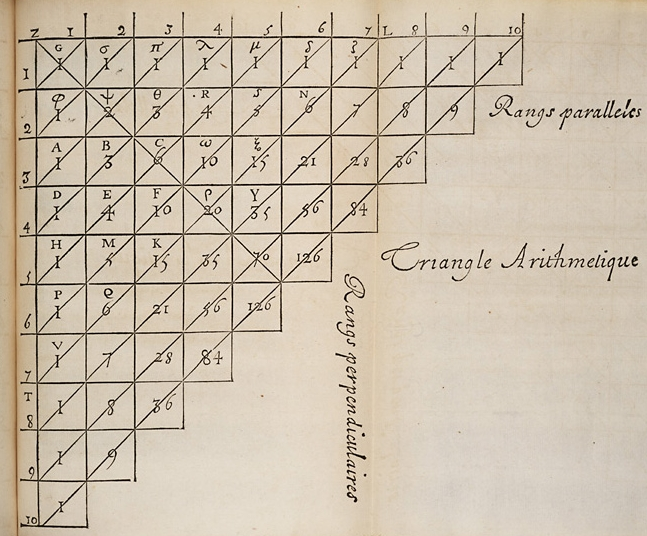
\includegraphics[width=0.8\textwidth]{TrianguloPascal.jpg}
\end{center}
\pagestyle{empty}




\newpage
\pagestyle{empty}
\tableofcontents
\vfill
\tr|Dieses Skript basiert teilweise auf einem Skript geschrieben von Irmgard Bühler, 
    welches wiederum auf einem Skript von Armin Barth (MINT-Lernzentrum ETH Zürich) 
    basiert. Einige der Aufgaben aus Irmgards Skript stammen aus den Büchern 
   \emph{Rhyn, Stochastik}, und \emph{Lambacher Schweizer, Mathematik 11/12} and from 
   \emph{Mathematics for the international student, Mathematics HL (Core), Haese and Harris Publications}.
   |This script is partly based on a script written by Irmgard Bühler, 
   which is itself based on a  script written by Armin Barth, 
   MINT-Lernzentrum ETH Zürich. Some of the exercises in Irmgards script were taken from the books 
   \emph{Rhyn, Stochastik}, and \emph{Lambacher Schweizer, Mathematik 11/12} and from 
   \emph{Mathematics for the international student, Mathematics HL (Core), Haese and Harris Publications}.|

   \tr|Alle verbleibenden Fehler sind -- natürlich -- meine. | All remaining mistakes are -- of course --  mine. |

\newpage

\pagenumbering{arabic}
\pagestyle{fancy} %eigener Seitenstil
\fancyhf{} %alle Kopf- und Fußzeilenfelder bereinigen
\fancyhead[L]{\tr|Wahrscheinlichkeit|Probability Theory|} %Kopfzeile links
%\fancyhead[R]{\leftmark} %zentrierte Kopfzeile
\fancyhead[C]{} %Kopfzeile rechts
\renewcommand{\headrulewidth}{0.4pt} %obere Trennlinie
\fancyfoot[C]{\thepage} %Seitennummer
%\renewcommand{\footrulewidth}{0.4pt} %untere Trennlinie
\setlength{\headheight}{13.6pt} 





\newpage
% Front:1 ends here

% [[file:../scripts.org::*Intro Examples][Intro Examples:1]]
\section{\tr|Prolog|Prologue|}
\begin{exc}
  \textbf{\tr|Bedingte Wahrscheinlichkeit|Conditional probability|:}
    \tr|Jemand hat zwei Kinder, eines davon ist ein Junge. Wie gross ist die Wahrscheinlichkeit,
      dass er zwei Jungen hat?
      |Somebody has two kids, one of them is a boy. What is the probability that he has two boys?|
\end{exc}
\begin{Answer}
  \tr|Eine h"aufige Antwort ist 0.5, vielleicht, weil die Frage folgendermassen verstanden wird:
  |A frequent answer is  0.5, maybe because one  understands the question as:|
  \begin{quote}
    \emph{\tr|Wenn ich schon einen Jungen habe, was ist die Wahrscheinlichkeit, 
      dass das n"achste Kind auch ein Junge ist?
      |I already have a boy, whats the probability that my next child will be a boy?|} 
  \end{quote}
  \tr|Die Konfigurationen ($M$=M"adchen, $J$=Junge) 
  $$
  (M,M),\quad(M,J),\quad(J,M),\quad(J,J),\quad
  $$
  haben alle die gleiche Wahrscheinlichkeit.
  Ok, genau genommen wissen wir das nicht, aber gehen wir der Einfachheit halber davon aus.
  Drei davon enthalten mindestens einen Jungen,
  und von denen enth"alt wiederum nur eine zwei Jungen, also ist die gesuchte 
  Wahrscheinlichkeit $\frac13$.
  |But the configurations ($G$=Girl, $B$=Boy)
  $$
  (G,G),\quad(G,B),\quad(B,G),\quad(B,B),\quad
  $$
  all have equal probability.
  Strictly speaking we cannot be sure about this. But lets assume this for the sake of simplicity.
  Three of them contain at least one boy and only one of the 
  contains two boys. Hence the probability is $\frac13$. |
\end{Answer}
\answerline{5}
\begin{exc}
  \textbf{\tr|D'Alemberts Fehler|D'Alembert's misstep:|} 
  Jean le Rond d'Alembert (1717-1783) 
  \tr|einer der bekanntesten Intellektuellen seiner Zeit und Mitherausgeber der 
  \emph{Encyclop\'edie} betrachtete dort das folgende Problem:
  |one of the foremost intellectual of the eighteenth century,
  co-editor of the Encyclop\'edie, considered the following problem there:|
  \begin{quote}
    \tr|Wenn man eine faire M"unze zweimal wirft, was ist die Wahrscheinlichkeit, 
        mindestens einmal Kopf zu werfen?
       |In two tosses of a fair coin, what is the probability that heads will appear at least once?|
  \end{quote}
  \tr|Er argumentierte, dass im echtem Leben niemand weiterspielen w"urde wenn beim ersten Wurf Kopf erscheint. 
      Mit anderen Worten betrachtete d'Alambert nur die folgenden Resultate $K$, $ZK$, $ZZ$
      und kam auf die  Antwort $\frac23$. Wo liegt der Fehler?
     |He reasoned that in real life no one would continue the experiment after heads showed up on the first toss. 
      In other words, d'Alembert's considered only the outcomes  $H$, $TH$, $TT$, prompting the answer $\frac23$.
      What's wrong here?|
\end{exc}
\answerline{5}
\begin{exc}
  \textbf{\tr|Geburtstagsparadoxon|Birthday problem|:} 
  \tr| \aside{Auf diesem  Resultat basiert auch eine kryptographische Technik, der sogenannte \emph{Geburtstagsangriff}.} 
  Wieviele Sch"uler muss eine Klasse haben, so dass die Wahrscheinlichkeit, dass mindestens zwei der Sch"uler
  am gleichen Tag Geburtstag haben mindestens 50\% ist? 
  Sie m"ussen diese Frage noch nicht beantworten k"onnen. Versuchen Sie die Antwort zu sch"atzen.
  | \aside{There is a cryptographic technique based on this: the \emph{birthday attack}}|
  How many people have to be in a class so that the probability that at least some pair 
  will have the same birthday is $\geq50\%$. At the moment, it is probably too hard to answer this question.
  Just guess.|
\end{exc}
\begin{Answer}
  \tr|Siehe Übung \ref{birthday}|See exercise \ref{birthday}| 
\end{Answer}
\answerline{5}
\xwrap{0}{
\begin{exc}
  \textbf{Monty Hall Problem:}
  \tr|Basierend auf der amerikanischen Fernsehshow \emph{Let's Make a Deal} und benannt nach dessen Showmaster,
      Monty Hall:
     |Loosely based on the American television game show \emph{Let's Make a Deal} and named after its original
      host, Monty Hall:|
  \begin{quote}
    \tr|Sie nehmen an einer Spielshow teil und k"onnen eine von drei T"uren ausw"ahlen.
    Hinter einer T"ure ist ein Auto, hinter den anderen Ziegen.
    Sie w"ahlen eine T"ure, z.B. Nr. 1 und der Showmaster (der weiss was sich hinter welcher T"ure
    verbirgt) "offnet eine andere T"ure, z.B. Nr. 3 hinter der eine Ziege steckt. Und dann fragt er: 
    ``M"ochten Sie lieber T"ure Nr. 2 "offnen?''.
    Ist es besser zu wechseln oder spielt das keine Rolle?
   |Suppose you're on a game show, and you're given the choice of three doors:
    Behind one door is a car; behind the others, goats.
    You pick a door, say No. 1, and the host, who knows what's behind the doors, opens another door, 
    say No. 3, which has a goat.
    He then says to you, ``Do you want to pick door No. 2?'' Is it to your advantage to switch your choice?|
  \end{quote}
\end{exc}
\begin{Answer}
  \tr|Das Problem wurde ber"uhmt durch einen Leserbrief in Marilyn vos Savants Kolummne ``Ask Marilyn''
  im \emph{Parade} Magazin im Jahre 1990.
  Vos Savants Antowrt war, dass der Teilnehmer die T"ure wechseln sollte, weil sich dann seine
  Gewinnchancen verdoppeln.
  Daraufhin gingen ca. 10000 Leserbriefe bei \emph{Parade} ein (und fast 1000 davon von Lesern
  mit einem  Doktortitel), von denen die meisten behaupteten, dass vos Savants sich irre,
  Paul Erd"os, einer der bekanntesten Mathematiker seiner Zeit, liess sich erst von einer
  Computersimulation "uberzeugen. 
  |It became famous as a question from a reader's letter quoted in Marilyn vos Savant's ``Ask Marilyn''
  column in \emph{Parade} magazine in 1990. 
  Vos Savant's response was that the contestant should switch to the other door:
  contestants who switch have a 2/3 chance of winning the car, 
  while contestants who stick to their choice have only a 1/3 chance.
  After the problem appeared in Parade, approximately 10,000 readers,
  including nearly 1,000 with PhDs,
  wrote to the magazine, most of them claiming vos Savant was wrong. 
  Paul Erd\"os, one of the most prolific mathematicians in history,
  remained unconvinced until he was shown a computer simulation confirming the predicted result.|
\end{Answer}
\answerline{5}}
\begin{exc}
  \textbf{\tr|Seltene Krankheiten|Rare diseases|:}
  \tr|\emph{Morbus} ist ein seltene Krankheit, nur eine von 10'000 Personen hat sie. 
     Ein Test für \emph{Morbus} ist
     |\emph{Morbus} a rare disease. Only one person out of 10'000  has it. A test for morbus is|
  \begin{itemize}
  \item \tr|postitiv mit 90\% Wahrscheinlichkeit, falls die Person krank ist,
           |positiv with 90\% if a person is sick.|
  \item \tr|negativ mit 98\% Wahrscheinlichkeit, wenn die Person gesund ist. 
           |negativ with 98\% if a person is healthy.|
  \end{itemize}
  \tr|Ihr Test ist positiv. Sollten Sie sich Sorgen machen ? 
     |You get a positive test, should you worry?|
\end{exc}
\begin{Answer}
   \tr|Siehe Abschnitt \ref{cond}: Die Wahrscheinlickeit, dass Sie krank sind ist 0.45\%. 
      |See section \ref{cond}: Not really; the probability that you are sick is 0.45\%|
\end{Answer}
\answerline{5}
\begin{exc}\label{petersburgintro}
  \textbf{\tr|Das St. Petersburg Paradox|St. Petersburg paradoxon|:}
    \tr|Ein Casino bietet ein Glücksspiel an, bei dem in jeder Runde eine faire Münze geworfen wird. 
        Der Gewinn des Spielers beginnt bei 2 Dollar und wird in jeder Runde verdoppelt, 
        wenn \emph{Kopf} geworden wird.  
        Sobald \emph{Zahl} erscheint ist das Spiel zu Ende und der Spieler erhält seinen Gewinn ausbezahlt.
        D.h. der Spieler erhält 
        \begin{itemize}
        \item 2 Dollar, wenn im ersten Wurf \emph{Zahl} erscheint,  
        \item 4 Dollar, wenn im ersten Wurf \emph{Kopf} erscheint und im zweiten \emph{Zahl},  
        \item 8 Dollar, wenn in den ersten zwei  Würfen \emph{Kopf} erscheint und im dritten \emph{Zahl},  
        \item usw. 
        \end{itemize}
       |A casino offers a game of chance for a single player in which a fair coin is tossed at each stage.
        The pot starts at 2 dollars and is doubled every time a head appears.
        The first time a tail appears, the game ends and the player wins whatever is in the pot. 
        Thus the player wins
        \begin{itemize}
        \item 2 dollars if a tail appears on the first toss,
        \item 4 dollars if a head appears on the first toss and a tail on the second,
        \item 8 dollars if a head appears on the first two tosses and a tail on the third,  
        \item and so on. 
        \end{itemize}|
      \tr|Welchen Preis wären Sie bereit für dieses Spiel zu zahlen?
         |What would be a fair price to pay the casino for entering the game?|
\end{exc}
\begin{Answer}
  \tr|Die erstaunliche Antwort ist: Man sollte diese Spiel zu jedem offerierten Preis zahlen.
     |The astonishing answer is:  one should  play the game at any price if offered the opportunity.
     From Wikipedia:
     \emph{Although this paradox is three centuries old, new arguments are still being introduced.}|
  \tr|Siehe Übung \ref{petersburg}.
     |See exercise \ref{petersburg}.|
\end{Answer}
\answerline{5}
\begin{exc}
  \textbf{\tr|Rationale Zahlen|Rational numbers|:}
  \tr|Wir ziehen zufällig eine reelle Zahle zwischen 0 und 1. Wie gross ist die Wahrscheinlichkeit,
  dass die gezogene Zahl rational ist?
  |Assume we randomly pick a number between 0 and 1,
  whats the probability that it is a rational number? |
\end{exc}
\begin{Answer}
  \tr|Erstaunlicherweise ist die Antwort 0. Das ist nicht sehr intuitiv, weil die gezogene Zahl ja
  sehr wohl rational sein könnte, also sollte die Wahrscheinlickeit nicht 0 sein.
  Ganz kurz gefasst geht das Argument folgendermassen:
  Nehmen wir an, die Wahrscheinlichkeit eine ganz bestimmte rationale Zahl (z.B. $\frac12$) zu ziehen sei
  eine kleine aber positive Zahl (z.B. $\frac1{1000000}$). Diese Wahrscheinlichkeit sollte die gleiche sein für
  jede andere rationale Zahl. Aber es gibt unendlich viele rationale Zahlen zwischen 0 und 1  und deshalb
  wäre die Wahrscheinlichkeit irgendeine rationale Zahl zu ziehen die Summe dieser Wahrscheinlichkeiten:
  Unendlich. 
  |Astonishingly the answer is 0. This is somewhat counter-intuitive, because if you just draw a number randomly,
  this number could be rational, hence the probability to do so should not be 0. Here's the argument in a
  nutshell: Assume the probability to choose some specific rational numer, e.g. $\frac12$,
  is a small, but positive number, let's say $\frac1{1000000}$. This probability should be the same
  for any rational number. But there are infinitly many rational numbers, hence this would imply that the
  probability to choose just some rational number would be the sum of these probabilties: infinity. |
\newpage
\end{Answer}
\answerline{5}
\par\bigskip\bigskip



\newpage
\tr|\emph{Wahrscheinlichkeit} als mathematische Disziplin ist erstaunlich neu: 
    Sie beginnt mit einem Briefwechsel zwischen \emph{Pierre der Fermat} und \emph{Blaise Pascal} 
    %\aside{Ja, es sind wirklich die beiden, Fermat mit dem  \emph{Fermatscher Satz} und Pascal mit dem \emph{Pascal'schen Dreieck}} 
     im Jahr 1654. Wir können nur spekulieren, warum dies so spät geschah, denn Glücksspiele wurden zu allen 
     Zeiten gespielt. Vielleicht fand man bis dahin, dass \emph{Zufall} in den Zuständigkeitsbereich der Götter fiel. 
    |Probability as a mathematical field entered the world astonishingly late:
    Aside from the elementary work by Cardano ($16^{\text{th}}$ century),
    the doctrine of probabilities dates to the correspondence of Pierre de Fermat and Blaise Pascal (1654). 
    We can only speculate why this happened so late, as games of chance are much older.
    Maybe \emph{chance} was thought to belong to the realm of gods. |

\tr|Pascal und Fermat diskutierten, das (inzwischen) sogenannte \emph{Teilungsproblem} (ursprünglich gestellt von Luca Paciola (1494)).
   |Pascal and Fermat were discussing the (now) so called \emph{problem of points} (posed by  Luca Pacioli (1494)): |
% \aside{\tr|Falls Sie die Entwicklung der komplexen Zahlen kennen: Auch Cardano und Tartaglia haben Lösungen vorgeschlagen:
%            \href{https://de.wikipedia.org/wiki/Teilungsproblem}{Teilungsproblem}
%           |In case you heard about the development of complex numbers: Also Cardano and Tartaglia submitted solutions to this problem: 
%            \href{https://en.wikipedia.org/wiki/Problem_of_points}{Problem of points}|
%        }
\begin{quote}
  \tr|Beim Teilungsproblem geht es um ein (faires) Glücksspiel zwischen zwei Spielern, bei dem es in jeder Runde einen Sieger gibt
      (es ist also kein Unentscheiden möglich),  z.B. könnten die beiden Spieler ganz einfach mehrmals eine Münze werfen.
      Vor Spielbeginn zahlen beide Spieler den gleichen Einsatz ein. Der erste Spieler, der 3 Runden gewinnt bekommt den ganzen Einsatz, 
      Nehmen wir nun an, dass das Spiel unterbrochen werden muss bevor einer der beiden Spieler gewonnen hat. 
      Wie teilen die beiden Spieler den Einsatz nun gerechtesten auf?
     |The problem concerns a game of chance with two players who have equal chances of winning each round (no draws).
      The players contribute equally to a prize pot,
      and agree in advance that the first player to have won  3 rounds will collect the entire prize. 
      Now suppose that the game is interrupted by external circumstances before either player has achieved victory.
      How does one then divide the pot fairly? |
\end{quote}
\tr|Nehmen wir an, der Spieler $A$ hat die erste Runde gewonnen, bevor das Spiel unterbrochen wurde. Die folgende Tabelle enthält alle möglichen     Spielverläufe unter diesen Umstanden:
   |Lets assume that player $A$ has won the first round before interruption. The following table contains all possible gameplays under these circumstances: |
\par\medskip
\begin{center}
\begin{tabular}{rlll}		
   & \tr|Spielverlauf|Game| & \tr|Gewinner|Winner| & \tr|Wahrscheinlichkeit|Probability| \\[1ex]\hline
  1 & $A$ $A$ $A$ & $A$  & $\frac14$ \\[1ex]
  2 & $A$ $A$ $B$ $A$ & $A$ & $\frac1{8}$\\[1ex]
  3 & $A$ $A$ $B$ $B$ $A$ & $A$ &$\frac1{16}$ \\[1ex]
  4 & $A$ $A$ $B$ $B$ $B$ & $B$  & $\frac1{16}$\\[1ex]
  5 &$A$ $B$ $A$ $A$ & $A$ &$\frac1{8}$\\[1ex]
  6 &$A$ $B$ $A$ $B$ $A$ & $A$ & $\frac1{16}$\\[1ex]
  7 &$A$ $B$ $A$ $B$ $B$ & $B$ &$\frac1{16}$\\[1ex]
  8 &$A$ $B$ $B$ $A$ $A$ & $A$ &$\frac1{16}$\\[1ex]
  9 &$A$ $B$ $B$ $A$ $B$ & $B$ & $\frac1{16}$\\[1ex]
  10& $A$ $B$ $B$ $B$  & $B$& $\frac1{8}$\\[1ex]
\end{tabular}
\end{center}
\par
\begin{align*}
  P(\text{$B$ \tr|gewinnt|wins|})&=\frac5{16}	\\
  P(\text{$A$ \tr|gewinnt|wins|})&=\frac{11}{16}	
\end{align*}
\tr|Sie sollten also den Einsatz im Verhaltniss 5:11 teilen.| Hence they should share the money in a 5:11 ratio.|


\newpage
% Intro Examples:1 ends here

% [[file:../scripts.org::*Basic Terms][Basic Terms:1]]
\section{\tr|Grundlagen|Basic Terms|}
\tr|Der erste Schritt zu einer mathematischen Theorie der Wahrscheinlichkeit ist die Einsicht, das Fragen zur Wahrscheinlichkeit immer Fragen 
    zur \emph{relativen Grösse von Mengen} sind. Z.B. geht es in \emph{D'Alemberts Fehler} um die Gr"osse der Menge
    $$\{(K,Z), (Z,K), (K,K)\}$$ 
    im Verh"altnis zur Gr"osse der Menge 
    $$\{(K,Z), (Z,K), (K,K), (Z,Z)\}$$  
    Oft (aber nicht immer) kann die Gr"osse einer 
    Menge ganz einfach durch Z"ahlen bestimmt werden und deshalb haben wir uns im Kapitel 'Kombinatork' mit Z"ahltechniken besch"aftigt. 
   |The first step 
    in formalising probability is to see that all problems about probabilities can be seen as questions on the (relative) size of some sets.  
    e.g. in \emph{d'Alembert's misstep:} the size of $\{(H,T), (T,H), (H,H)\}$ versus the size of $\{(H,T), (T,H), (H,H), (T,T)\}$. 
    Often (but not always) these sizes can be determined by merely counting and thats why the previous chapter was about \emph{Counting techniques} or \emph{Combinatorics}.|
% \aside{
% \tr|Man kann auch das Problem der \emph{seltenen Krankheiten} durch Z"ahlen l"osen: Nehmen wir an,  1 Million Menschen haben den Test gemacht. 
%     100 von ihnen haben die Krankheit. Von diesen 100 Kranken haben 90 einen positiven Test. 
%     Von den restlichen 999'9000 Gesunden haben 979902 (98\%) einen negativen Test und 19998 einen positiven Test. Insgesamt haben also 20088 einen positiven Tes. 
%     Davon sind aber nur 90 wirklich wirklich krank: $\frac{90}{20088}\approx0.0045$.
%    |You can also solve \emph{the rare disease} problem by counting: Assume 1Milllion people did the test. 100 of them are sick. 90 of them have a positive test. 
%     999'900 are healthy  and 979902 of them have a negative test, 19998 a positive test. Together, 20088 have positive test, 90 of them are sick.
%     The relative size of 90 people in 20088 is approx. 0.0045.|
% }
\par\bigskip\bigskip
\tr|Um Wahrscheinlichkeitsprobleme in Mengen übersetzen zu können, brauchen wir zuerst einen geeigneten Jargon: 
    In der folgenden Tabelle werden diese Grundbegriffe definiert und jeweils am Beispiel eines Würfels illustriert. 
   |Here a few first basic terms of probability theory. We illustrate their meaning using the random experiment of throwing a die. |
\vsp

\renewcommand{\arraystretch}{2}
{\footnotesize
\begin{tabular}{p{4.2cm}|p{4cm}|p{4.5cm}}
\hline
\hline
\textbf{\tr|Zufallsexperiment|Random experiment|:} &
\tr|Ein Experiment, dessen Ausgang nicht vorhergesagt werden kann. |An experiment in which the outcome cannot be predicted.|& 
\tr|Würfel werfen|die throwing|\\
\hline
\hline
\textbf{\tr|Ergebnis|Outcome|  $\omega$:} & \tr|Ein möglicher Ausgang des Experiments.| One of the possible outcomes of the experiment.|& $2$\\
\hline
\textbf{\tr|Ergebnismenge|Sample space| $\Omega$:} &
\tr|Menge aller möglichen Ergebnisse einers Zufallsexperiments.|Set of all possible outcomes of a random experiment.|  & 
$\Omega=\{1,2,3,4,5,6\}$\\
\hline
\hline
\textbf{\tr|Ereignis|Event|  $E$:} & \tr|Teilmenge von |Subset of | $\Omega$ & \parbox[t]{4.5cm}{\tr|Ein Vielfaches von 3 werfen,\\ d.h. |Throw a multiple of 3, \\ i.e. | $E=\{3,6\}$} \\
\hline
\textbf{\tr|Elementarerignis|Elementary event|:} & \tr|Eine Teilmenge von $\Omega$, die nur ein Element enthält.|A subset of $\Omega$, that contains only a single outcome.| & $E=\{2\}$\\
\hline
\hline
\textbf{\tr|Sich ausschliessende Ereignisse|Mutually exclusive events|:} & $E\cap F = \emptyset$ &
\parbox[t]{4.5cm}{ $E$ \tr|alle geraden Zahlen|all even numbers|, \\ $F$ \tr|alle ungeraden Zahlen|all odd numbers|\\ }\\
\hline
\textbf{\tr|Ereignis |Event | $E$ \tr|und |and | $F$:} & $E\cap F$ & \parbox[t]{4.5cm}{ \tr|gerades Resultat und \\Vielfaches von 3 d.h. |even result and \\multiple of 3, i.e. |
\\ $E=\{2,4,6\}$, $F=\{3,6\}$ \\ \tr|und |and | $E\cap F=\{6\}$ \\ }\\
\hline
\textbf{\tr|Ereignis |Event |$E$ \tr|oder |or | $F$:} & $E \cup F$ &\parbox[t]{4.5cm}{ \tr|gerades Resultat oder \\Vielfaches von 3 d.h. |even result or  \\multiple of 3, i.e. |
 \\$\{2,3,4,6\}$\\ }\\
\hline
\textbf{\tr|Gegenereignis |Complement of an event |$\bar{E}$:} & $\Omega \setminus E$ & \parbox[t]{4.5cm}{\tr|Resultat nicht gerade:|result not even:|
\\ $E=$\\$=\{1,2,3,4,5,6\} \setminus \{2,4,6\}$\\$=\{1,3,5\}$ \\ }\\
\hline
\hline
\end{tabular}
}
\vspace{1cm}

\newpage
\begin{exc}
\tr|Eine Münze wird dreimal geworfen und das Resultat (Kopf oder Zahl) wird jedesmal notiert. 
   |A coin is thrown three times in a row and the result (head or tail) is noted each time. |
\begin{enumerate}
\item \tr|Beschreiben Sie den Ereignisraum.|Describe the sample space.|
\answerline{1}
\item \tr|Geben Sie je ein Beispiel für ein Ergebnis und ein Ereignis an.| Write down an example of an outcome and an event.|
\answerline{2}
\item \tr|Geben Sie Beispiele zweier sich ausschliessender Ereignisse und zweier sich nicht ausschliessender Ereignisse an.
         |Give an example of two mutually exclusive events and of two events which are not mutually exclusive. |
\answerline{4}
\item \tr|Beschreiben Sie die folgenden Ereignisse als Teilmengen der Ereignismenge:| Describe the following events as a subset of the sample space.|
\begin{itemize}
\item \tr|Wir werfen die gleiche Seite dreimal.|We throw the same side three times.|
\answerline{1}
\item \tr|Kopf erscheint genau einmal.| A head occurs exactly once.|
\answerline{1}
\item \tr|Zahl erscheint höchstens einmal.| A tail occurs at most once.|
\answerline{1}
\item \tr|Kopf erscheint mindestens zweimal.| A head occurs at least twice.|
\answerline{1}
\end{itemize}
\item \tr|Was sind die Gegenereignisse der obigen Ereignisse?| What are the complementary events to the above-mentioned events?|
\answerline{4}
\item \tr|Welches Ereignis beschreibt das Auftreten des ersten \emph{und} des dritten  der obigen Ereignisse?
         |Which event describes the occurrence of the first \emph{and} third event as mentioned above?|
\answerline{4}
\item \tr|Welches Ereignis beschreibt das Auftreten des ersten \emph{oder} des dritten  der obigen Ereignisse?
         |Which event describes the occurrence of the first \emph{or} third event as mentioned above?|
\answerline{4}
\end{enumerate}
\end{exc}
\begin{Answer}
  \begin{enumerate}
  \item
     \tr|$\Omega=\{KKK, KKZ, KZK, ZKK, KZZ, ZKZ, ZZK, ZZZ\}$ 
     |$\Omega=\{HHH, HHT, HTH, THH, HTT, THT, TTH, TTT\}$ |
   \item
     \tr|$\omega=KKZ$\\ $E=\{KKK, ZKK, ZZK\}$
        |$\omega=HHT$\\ $E=\{HHH, THH, TTH\}$|
   \item
     \tr|\begin{align*}
           E_1&=\{KKK,ZZZ\}\\
           E_2&=\{KKZ,KZK,ZKK\}\\
           E_3&=\{KKK,KKZ,KZK,ZKK\}\\
           E_1\cap E_2&=\{\}\\
           E_1\cap E_3&=\{KKK\}
         \end{align*}
        |\begin{align*}
           E_1&=\{HHH,TTT\}\\
           E_2&=\{HHT,HTH,THH\}\\
           E_3&=\{HHH,HHT,HTH,THH\}\\
           E_1\cap E_2&=\{\}\\
           E_1\cap E_3&=\{HHH\}
         \end{align*}|
    \item
     \tr|\begin{align*}
           E_1&=\{KKK,ZZZ\}\\
           E_2&=\{KZZ,ZKZ,ZZK\}\\
           E_3&=\{KKK,KKZ,KZK,ZKK\}\\
           E_4&=E_3
         \end{align*}
        |\begin{align*}
           E_1&=\{HHH,TTT\}\\
           E_2&=\{HTT,THT,TTH\}\\
           E_3&=\{HHH,HHT,HTH,THH\}\\
           E_4&=E_3
         \end{align*}|
    \item
     \tr|\begin{align*}
           \bar{E_1}&=\{KKZ, KZK, ZKK, ZZK, ZKZ, KZZ\}\\
           \bar{E_2}&=\{KKK,KKZ, KZK, ZKK, ZZZ\}\\
           \bar{E_3}&=\{ZZZ,ZZK, ZKZ, KZZ\}\\
           \bar{E_4}&=\bar{E_3}
         \end{align*}
        |\begin{align*}
           \bar{E_1}&=\{HHT, HTH, THH, TTH, THT, HTT\}\\
           \bar{E_2}&=\{HHH,HHT, HTH, THH, TTT\}\\
           \bar{E_3}&=\{TTT,TTH, THT, HTT\}\\
           \bar{E_4}&=\bar{E_3}
         \end{align*}|
    \item 
      \tr|$E_1\cap E_3=\{KKK\}$|$E_1\cap E_3=\{HHH\}$|
    \item
      \tr|$E_1\cup E_3=\{KKK, KKZ,KZK,KKZ,ZZZ\}$
         |$E_1\cup E_3=\{HHH, HHT,HTH,HHT,TTT\}$|
  \end{enumerate}
\newpage
\end{Answer}
\newpage
% Basic Terms:1 ends here

% [[file:../scripts.org::*Axioms][Axioms:1]]
\section{\tr|Axiome|Axioms of probability|}
\subsection*{\tr|Wenn zählen nichts nützt|When counting fails|}
\begin{exc}
  \tr|Sie schiessen Pfeile auf die folgende Zielscheibe: 
  |You shoot arrows at the following target: |
  \begin{center}
    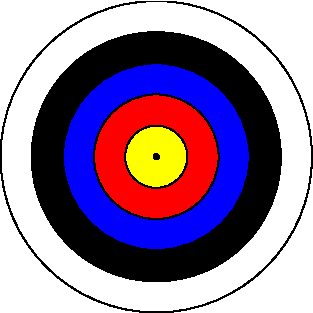
\includegraphics[width=0.3\textwidth]{target.pdf}
  \end{center}
  \tr|Vereinfachen wir etwas und nehmen an, dass die Kreisringe alle gleich 'dick' sind.
  |Let's simplify a bit and
  assume that all rings have equal 'thickness'.|
  \tr|Nehmen wir an Sie sind ein m"assig guter Bogensch"utze: Sie treffen zwar immmer die Scheibe,
  aber abgesehen davon ist es reiner Zufall, wohin der Pfeil geht.
  |Let's assume you are a moderate archer: you always hit the target, but besides this, the exact position is absolutely random.|
  \begin{enumerate}
  \item \tr|Was ist die Wahrscheinlichkeit, dass Sie die linke H"alfte der Scheibe treffen?
    |What is the probability that you hit the left half of the target?|
    \answerline{1}
  \item \tr|Was ist die Wahrscheinlichkeit, dass Sie den gelben Teil der Scheibe treffen? 
    |What is the probability that you hit the yellow part of the target?|
    \answerline{1}
  \item \tr|Nehmen wir an, Sie sind ein hervorragender Bogenschütze, und treffen weitaus öfters ins Zentrum der Scheibe als in den Randbereich. 
    Welche der obigen Fragen können Sie noch beantworten? Welche Informationen fehlen Ihnen?
    |Let's assume you are a talented archer and hit the center more often than the border. 
    Which of the above questions can you answer and what informations are missing?|
    \answerline{2}
  \end{enumerate}
\end{exc}
\begin{Answer}
  \begin{enumerate}
  \item $\frac12$ 
  \item 
    \tr|Der Radius des gelben Teils ist $\frac 15$ des Radius' der ganzen Scheibe, also ist seine
        Fläche $\left(\frac15\right)^2$ der ganzen Fläche. 
       |The radius is $\frac15$ of the radius of the whole disc, hence it's area is $\left(\frac15\right)^2$ of the total area. |
  \item
   \tr|Die Antwort auf die erste Frage bleibt gleich, aber für die zweite Frage müssten wir genauer wissen, wie gut Sie treffen.  
      |The answer for the first question stays the same, but for the second question we have some quantitative knowledge on your archery skills. |
  \end{enumerate}
\end{Answer}
\tr|Einerseits lassen sich Wahrscheinlichkeiten durch Zählen berechnen, andrerseits auch durch eine Art \emph{Flächenberechnung}. Wie lässt sich all dies in einem Konzept behandeln?
|On one hand probabilty is like \emph{counting}  on the other hand like \emph{area} or worse like a weighted area. 
How can we summarize all this in one concept?|

\tr|Etwa im Jahr 1930 gab Kolmogorov ein solches Konzept an:
|Around 1930, Kolmogorov gave a formal definition of how to measure relative size of sets: |

\begin{ttile}{\tr|Wahrscheinlichkeits-Axiome|Axioms of probability|}
  \tr|Sei $\Omega$ eine Menge. Eine Funktion $P$, die jeder Teilmenge $A$ von $\Omega$ eine reelle Zahl zuordnet heisst
  \emph{Wahrscheinlichkeit}, falls gilt:
  |Assume $\Omega$ is a set.
  A function $P$ that assigns a real number to any subset $A$ of $\Omega$  is called a \emph{probability} if|
  \begin{itemize}
  \item[($P_1$)] $P(A)\geq 0$   \tr|f"ur alle Teilmengen |for all subsets $A\subset \Omega$|
  \item[($P_2$)] $P(\Omega)=1$ 
  \item[($P_3$)] $P(A\cup B)=P(A)+P(B)$ 
    %\aside{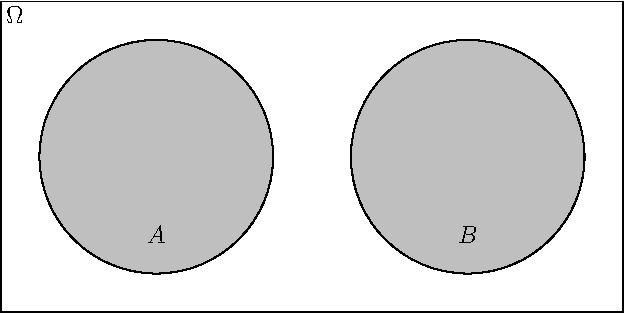
\includegraphics[width=4cm]{venn_disjoint.pdf}}
    % \aside{\tr|Das ist eigentlich nur die 'endliche' Version dieses Axioms und oft braucht man die 'unendliche' Version
    %   mit einer ganzen Folge von gegenseitig disjunkten Menge. 
    %   |Actually this is just the 'finite' version and often one needs an 'infinite' version
    %   involving a sequence of mutually disjoint sets, that is every pair of sets is disjoint.|
    %}
    \tr|wenn $A$ und $B$ disjunkt sind, d. h. falls sie keine Elemente gemeinsam haben: $A\cap B=\{\}$ 
    |if $A$ and $B$ are disjoint, that is if they have no elements in common, that is if $A\cap B=\{\}$| 
  \end{itemize}
\end{ttile}

\begin{example}
  \tr|In \emph{d'Alemberts Fehler} wäre die Ergebnismenge
  |In  \emph{d'Alembert's misstep:} the sample space would be |
  $$
  \Omega=\{(H,T), (T,H), (H,H), (T,T)\}
  $$
  \tr|und ein mögliches Ereignis |and a possible event |
  $$
  A=\{(H,T), (T,H), (H,H)\}
  $$
  \tr|und die Wahrscheinlichkeitsfunktion |and the probability function |
  $$
  P(A)=\frac{\text{\tr|Anzahl Elemente von|number of elements in| $A$}}{\text{\tr|Anzahl Elemente von |number of elements in| $\Omega$}}
  $$
\end{example}
\par 
% add in next version <<next-version>>

%\begin{exc}
% \tr|In einem Behälter befinden sich Kugeln von denen jede mit einem der Buchstaben 'a', 'b', 'c' und  'd'  beschriftet ist. 
%     Diese Kugeln werden nun sehr oft gezogen und wieder zurückgelegt. Es stellt sich heraus, dass die Buchstaben 'a', 'b', 'c', und 'd' im Verhältnis 
%    7:4:6:8 gezogen werden. Geben Sie eine passende Wahrschenlichkeitsfunktion an. 
% | There are balls in a box, each bearing one of the letters a, b, c, d. The balls were drawn many times. 
% Each time, the letter on the ball was written down, then the ball was put back and all balls were mixed again. 
% It was found that the letters a, b, c and d were drawn in a ratio of 7:4:6:8. Specify an appropriate probability distribution.|
% \end{exc}
% \begin{Answer}
%   \begin{align*}
%     P(\{a\})&=7/25\\
%     P(\{b\})&=4/25\\
%     P(\{c\})&=6/25\\
%     P(\{d\})&=8/25\\
%   \end{align*}
% \end{Answer}
\tr|Diese Axiome haben einige unmittelbare Konsequenzen, die Eigenschaften von \emph{Wahrscheinlichkeit}, die ganz natürlich erscheinen:
(und das überraschende ist, dass wir wirklich nur diese Axiome brauchen, um sie zu beweisen.)
|These axioms have some immediate consequences describing 'facts' about probability that seeem quite natural: 
(and the surprising thing is: we really need only these axioms to prove these statements)|
\begin{prop}
  \tr|Wenn $P$ ein Wahrscheinlichkeitsfunktion auf $\Omega$ ist, und $A,B\subset\Omega$ dann gilt
  |If $P$ is a probability function on $\Omega$ and  $A,B\subset \Omega$ then|
  \begin{enumerate}
  \item $P(\{\})=0$
  \item $P(\Omega\setminus A)=1-P(A)$
    \marginpar{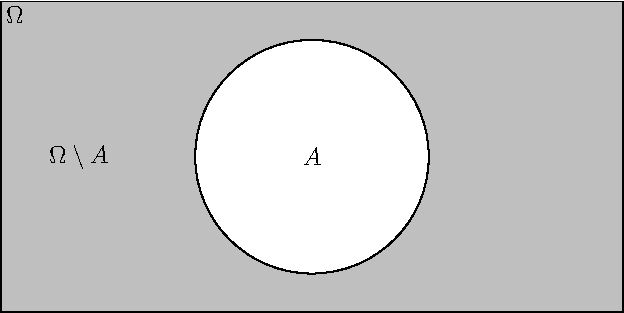
\includegraphics[width=4cm]{venn_complement.pdf}}
  \item $A\subset B\implies P(A)\leq P(B)$
  \item $0\leq P(A)\leq 1$
  \item $P(A\setminus B)=P(A)-P(A\cap B)$
    \marginpar{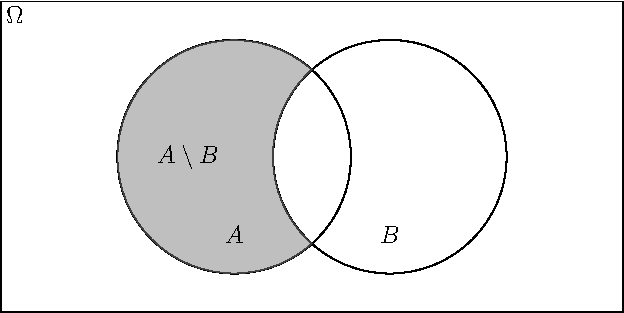
\includegraphics[width=4cm]{venn_without.pdf}}
  \item $P(A\cup B)=P(A)+P(B)-P(A\cap B)$
    \marginpar{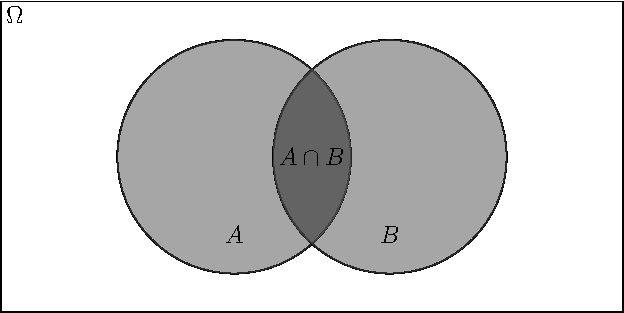
\includegraphics[width=4cm]{venn_inter.pdf}}
  \end{enumerate}
\end{prop}
\begin{proof}
  \tr|Wir haben nicht viel zur Hand, was wir brauchen könnten um  diese Aussagen beweisen zu können, ausser Mengenlehre und die obigen Axiome.
  |We don't have much tools to prove these statements except set theory and the three axioms|
  \begin{enumerate}
  \item 
    \tr|Die Zerlegung $\Omega=\Omega\cup\{\}$ ist disjunkt (d.h. ein Vereinigung zweier disjunkter Mengen) und deshalb gilt nach Axiom $(P_3)$ 
    |The decomposition $\Omega=\Omega\cup\{\}$ is a disjoint union  (that is a union of two disjoint sets) and therefore by axiom $(P_3)$| 
    \begin{align*}
      P(\Omega)&=P(\Omega)+P(\{\})\\
      1&=1+P(\{\})
    \end{align*}
    \tr|und daraus folgt | which implies | $P(\{\})=0$
  \item
    \tr|Dieses Mal ist die Zerlegung | This time the decomposition | $\Omega=A\cup (\Omega\setminus A)$ \tr|disjunkt | is a disjoint union|
    \begin{align*}
      P(\Omega)&=P(A)+P(\Omega\setminus A)\quad\text{\tr|nach | by | $(P_3)$} \\
      P(\Omega\setminus A)&=P(\Omega)-P(A)\\
               &=1-P(A) \quad\text{\tr|nach $(P)1$)| because of $(P_1)$|}
    \end{align*}
  \item 
    \begin{align*}
      B&=A\cup (B\setminus A )\quad\text{ \tr|disjunkte Vereinigung|disjoint union|}\\
      P(B)&=P(A)+P(B\setminus A)\quad\text{\tr|nach | by | $(P_3)$} \\
       &\geq P(A) \quad\text{\tr|weil |since | $P(B\setminus A)\geq 0$ \tr|wegen |by axiom | $(P_1)$}				
    \end{align*}
  \item \tr|folgt aus |follows from | $\{\}\subset A\subset \Omega$  \tr|und dem letzten Resultat. |and the previous result.|
  \item 
    \begin{align*}
      A&=(A\setminus B)\cup(A\cap B)\quad\text{\tr|disjunkte Vereinigung|disjoint union|}\\			
      P(A)&=P(A\setminus B)+P(A\cap B)\quad\text{\tr|wegen |by | $(P_3)$}\\			
      P(A\setminus B)&=P(A)-P(A\cap B)
    \end{align*}
  \item 
    \begin{align*}
      A\cup B&=(A\setminus B)\cup B\quad\text{\tr|disjunkte Vereinigung|disjoint union|}\\			
      P(A\cup B)&=P(A\setminus B)+P(B)\quad\text{by $(P_3)$}\\			
      P(A\cup B)&=P(A)-P(A\cap B)+P(B)\quad\text{\tr|wegen dem letzen Resultat|by the previous result|}\\			
    \end{align*}
  \end{enumerate}
\end{proof}

\begin{remark}$\,$\\
  \begin{enumerate}
  \item \tr|Meist wird das dritte Axiom in seiner unendlichen Version verwendete: |Usually the third axiom must be extended to an infinite version: |
    \begin{quote}
      \tr|Wenn $A_1$, $A_2$, \ldots eine \textbf{Folge von paarweise disjunkten Mengen} ist, d.h. je zwei davon sind disjunkt, dann gilt:
         |If $A_1$, $A_2$, \ldots  is a \textbf{sequence of mutually disjoint sets} i.e. every two of them are mutually disjoint, then|
      $$
      P(A_1\cup A_2\cup \ldots)=P(A_1)+P(A_2)+\ldots
      $$
    \end{quote}
    \tr|Z.B. ist im \emph{St. Petersburg Paradox}:
       |E.g. in the \emph{St.Petersburg paradoxon}:|
    \begin{align*}
      \Omega=\{T,HT,HHT,HHHT,\ldots\}=\{H\}\cup\{HT\}\cup\{HHT\}\cup\ldots
    \end{align*}
    \tr|Und wenn Sie z.B. an der Wahrscheinlichkeit interessiert sind, nach einer geraden Anzahl \emph{Köpfen} zu gewinnen, dann brauchen Sie die unendliche 
        Version des dritten Axioms.
       |And if you are for example interested in the probability of winning after an even number of heads, then you need the infinite version of the third axiom.|
  \item 
    \tr|Die ganze Geschichte ist tatsächlich etwas verworrener: Für $\Omega=[0,1]\subset\R$ kann die Sache schiefgehen: Wenn wir annehmen, dass ausser den obigen 
        Axiome (mit der unendlichen Version des dritten Axioms) auch noch gelten soll, dass die Wahrscheinlichkeit einer Teilmenge $A$ gleich ist, wie die Wahrscheinlichkeit
        einer verschobenen Kopie von $A$, (eine solche Wahrscheinlichkeitsfunktion wird \emph{gleichmässig} genannt), dann kann -- leider -- eine solche Wahrscheinlichkeitsfunktion 
        nicht existieren, bzw. genauer: eine solche Wahrscheinlichkeitsfunktion kann nicht füra alle Teilmengen von $\Omega$ definiert sein. 
       |The whole story is actually a little bit darker than it looks at the moment: In the case $\Omega=[0,1]\subset\R$ things can go terribly wrong:  If we assume, 
        besides the above axioms (with the infinite version of the third axiom) that the probability of a subset $A$ is the same as the probability of a shifted copy $A+r$ 
        (so called uniform probability), then, sadly, no such function $P$ can exist: or more precisely: such a function $P$ cannot be defined for all subsets of $\Omega$. |
    \ifVITALI\par
    \tr|Hier ist das Argumtent in voller Kürze: | Here's the argument in a nutshell:|
    \begin{quote}
      \tr|Verbinden wir zunächst die beiden Endpunkte des Intervalls $[0,1]$ zu einem Kreis (um zu verhindern, dass das Verschieben von Teilmengen aus $\Omega$ herausführt). 
          Für einen gegebenen Punkt $x$ auf dem Kreis sei $O(x)$ die Menge aller Punkte $y$ auf dem Kreis, die mit $x$ einen Winkel einschliesst, der ein \emph{rationales Vielfaches
          von $\pi$} ist. Dieses sogenannte \emph{Orbit} von $x$ ist eine abzählbare Menge (warum?) und für $x$ und $y$ auf dem Kreis gibt es nur zwei Möglichkeiten (warum?): 
         |Let's connect the two endpoints of $[0,1]$ to a circle. 
          Now given a point $x$ on the circle let $O(x)$ be the set of all point $y$ on the circle such that the angle between $x$ and $y$ is a \emph{rational multiple of $\pi$}. 
          This so called \emph{orbit} of $x$ is a countable set (why?), and, given $x$ and $y$ on the circle there are only two possibilities:(why?) |
      \begin{itemize}
      \item $O(x)=O(y)$
      \item $O(x)$ \tr|und | and | $O(y) $ \tr|sind disjunkt|are disjoint|
      \end{itemize}
      \tr|Die Anzahl solcher Orbits ist überabzählbar (warum?) und diese Orbits sind disjunkt und ihre Vereinigung ist $\Omega$, der Kreis.
          Wählen wir aus jedem Orbit ein Element und nennen die Menge dieser Elemente $\mathcal{S}$. Erstaunlicherweise ist das der Schwachpunkt des Arguments.
          Sei $\mathcal{S}_\alpha$ die um den Winkel $\alpha$ gedrehte Kopie von $\mathcal{S}$, wobei $\alpha$ wieder ein rationales Vielfaches von $\pi$ ist. 
          Die Mengen $\mathcal{S}_\alpha$ sind disjunkt und ihre abzählbare Vereinigung überdeckt den Kreis (warum?).
         |Now, the number of such orbits is uncountable (why?) but these orbits are disjoint and there union is $\Omega$, the circle. 
          Let's pick one element of each orbit and define $\mathcal{S}$ to be the set of these elements. Astonishingly this is the weak point of the argument.
          Let $\mathcal{S}_\alpha$ be the rotated copy of $\mathcal S$ (rotated with angle $\alpha$, a rational multiple of $\pi$). 
          The sets $\mathcal{S}_\alpha$ are disjoint and their countable union covers the circle (why?) |
          \par
          \tr|Wir haben es geschafft, eine Folge von Mengen zu konstruieren, deren Vereinigung den Kreis überdeckt und diese Mengen sind 
              alles rotierte Varianten voneinander. Das ist alles was wir brauchen:
             |We have managed to construct a sequence of sets whose union covers the circle and these sets are rotational copies of each other. Thats all we need:|
      \begin{itemize}
      \item \tr|Da $P$ gleichmässig ist, haben alle $\mathcal{S}_\alpha$ die gleiche Wahrscheinlichkeit. 
               |Since $P$ is uniform, all $\mathcal{S}_\alpha$ have the same probability.|
      \item \tr|Wenn diese Wahrscheinlichkeit 0 ist, dann ist es auch die Wahrscheinlichkeit ihrer Vereinigung (dem Kreis) 
                nach dem dritten Axiom (in der unendlichen Version). 
               |If this probability is 0, then so is the probabilty of their union
                (which is the circle) by the third axiom, in its 'infinite' version.|
      \item \tr|Wenn diese Wahrscheinlichkeit nicht 0 ist, dass ist es nach dem zweiten Axiom eine positive Zahl und die Vereinigung der $\mathcal{S}_\alpha$ 
                hat unendliche Wahrscheinlichkeit, im Widerspruch zum ersten Axiom.
               |If this probability is not 0, then, by the second axiom,
                it is a positive number, and the union of the $\mathcal{S}_\alpha$ has inftinite
                probability contradicting the first axiom. |
      \end{itemize}
    \end{quote}
    \fi
  \end{enumerate}
\end{remark}
% Axioms:1 ends here

% [[file:../scripts.org::*Laplace experiment][Laplace experiment:1]]
\newpage
\section{\tr|Laplace-Experimente|Laplace Experiment|}
  
\begin{ttile}{\tr|Laplace-Experiment|Laplace experiment|}
$ $
\tr|Wenn die möglichen Ausgänge eines Zufallsexperiments alle gleich wahrscheinlich sind, so wird es ein Laplace-Experiment genannt. Für ein 
    Laplace-Experiment gilt:
   |If the outcomes of a random experiment are all equally likely, we call it a Laplace experiment. For Laplace experiments, we have|
\[
P(E)=\frac{|E|}{|\Omega|}=\frac{\text{\tr|Anzahl günstiger Ergebnisse|number of favorable outcomes|}}{\text{\tr|Anzahl möglicher Ergebnisse|number of possible outcomes|}}
\]
\trr;Der Term $|E|$ steht für die Anzahl Elemente in $E$ und$|\Omega|$ für die Anzahl Elemente in $\Omega$.   
   ;The term $|E|$ describes the number of elements in $E$ and $|\Omega|$ the numbers of elements in $\Omega$.;
\end{ttile}
  
  
\begin{example}
$ $
  
\begin{itemize}
\item 
   \tr|Wenn man einen Würfel wirft, macht man ein Laplace-Experiment. Jede Zahl zwischen $1$ und $6$ ist gleich wahrscheinlich. 
       Die Wahrscheinlichkeit eine $1$ zu werfen ist also $\frac16$ und das gleiche gilt für alle anderen möglichen Ausgänge.  
      |When throwing a die, we perform a Laplace experiment: 
       Each number between one and six is equally likely to occur. 
       The probability to throw a $1$ is therefore $\frac{1}{6}$ and the same is true for all possible numbers.|
  
\item 
   \tr|Wenn man einen Reissnagel wirft, so führt man \textbf{kein} Laplace-Experiment durch. Die verschiedenen Seiten eines Reissnagels landen nicht mit gleicher
       Wahrscheinlichkeit oben. 
      |When throwing a drawing pin, we do \textbf{not} perform a Laplace experiment: The different sides are not thrown equally often. |
\end{itemize}
\end{example}
\vfill
  
\begin{xxwrap}
\begin{exc}
\tr|Sind das Laplace-Experimente? Begründen Sie Ihre Antwort.| Is it a Laplace experiment? Justify it!|
\begin{enumerate}
\item \tr|Sie werfen ein regelmässiges Tetraeder.| Throw an equilateral tetrahedron.|
\item \tr|Sie werfen einen Legobaustein.|Throw a Lego brick.|
\item \tr|Sie werfen eine Münze.|Throw a coin.|
\end{enumerate}
\end{exc}
\begin{Answer}
  \begin{enumerate}
  \item
    \tr|Wenn man annimmt, das der Tetraeder vollständig gleichmässig ist, ja.
       |Assuming that the tetrahedron is \emph{entirely uniform},  yes. | 
   \item
     \tr|Nein, Legobausteine, sind nicht gleichmässig.| No. Lego bricks are not uniform.|
   \item
     \tr|Münzen werden allgemein als \emph{fair} angenommen (z.B. im Fussball), also ja.
        |Most people think that coins are \emph{fair} (at least football players do), hence yes.|
  \end{enumerate}
\end{Answer}
\answerline{12}
\end{xxwrap}
\vfill
  
\begin{xxwrap}
\begin{exc}
\tr|Sie wählen zufällig einen Buchstaben aus dem Wort \texttt{PROBABILITY}. Mit welcher Wahrscheinlichkeit ist es 
   |Out of the word \texttt{PROBABILITY} we randomly choose a letter. What is the probability that|
\begin{enumerate}
\item \tr|ein \texttt{R}|an  \texttt{R}|
\item \tr|ein \texttt{E}|an \texttt{E}|
\item \tr|ein \texttt{B}|a \texttt{B}|
\item \tr|ein Vokal, d.h. \texttt{A}, \texttt{E}, \texttt{I}, \texttt{O} oder \texttt{U}
         |a vowel (i.e. \texttt{A}, \texttt{E}, \texttt{I}, \texttt{O} or \texttt{U})|
\item \tr|ein \texttt{L} oder ein \texttt{Y} |a \texttt{L} or a \texttt{Y}|
\end{enumerate}
\tr||is chosen?|
\end{exc}
\begin{Answer}
  \begin{enumerate}
  \item $\frac 1{11}$
  \item $0$
  \item $\frac 2{11}$
  \item $\frac4{11}$
  \item $\frac2{11}$
  \end{enumerate}
\end{Answer}
\answerline{12}
\end{xxwrap}
\vfill
  
\begin{xxwrap}
\begin{exc}
\tr|Sie werfen einen Würfel dreimal. Verwenden Sie eine der Konsequenzen aus den Axiomen von Kolmogorov um die folgenden 
    Wahrscheinlichkeiten zu berechnen.
   |We throw a die three times. Use one of the  consequences of the  Kolmogorovs Axioms to calculate the probabilitiy that|
\begin{enumerate}
\item \tr|Die Zahl 1 erscheint mindestens einmal.|the number 1 appears at least once. |
\item \tr|Die Zahl 3 erscheint höchstens zweimal.|the number 3 appears at most twice.|
\item \tr|Die Summe der drei Würfe ist nicht 5.|the sum of the three throws is not 5.  |
\end{enumerate}
\end{exc}
\begin{Answer}
  \begin{enumerate}
  \item
    $$P(\text{\tr|mindestens eine 1|at least once a 1|})=
    1-P(\text{\tr|nie eine 1|never  a 1|})=1-\left(\frac56\right)^3\approx 0.42$$
  \item
    $$P(\text{\tr|3 h\"ochstens zweimal|3 at most twice|})=1-P(\text{\tr|dreimal 3|three times 3|})=1-\left(\frac16\right)^3\approx 0.995$$
  \item 
    $$P(\text{\tr|Summe ist nicht 5|Sum is not 5|})=1-P(\text{\tr|Summe ist 5|sum is 5|})=1-3\left(\left(\frac16\right)^3+\left(\frac16\right)^3\right)\approx 0.972$$
    \tr|weil|because |
    \begin{align*}
     5&=1+1+3\\ 
     5&=2+2+1 
    \end{align*}
  \end{enumerate}
\end{Answer}
\answerline{12}
\end{xxwrap}
\vfill


\begin{xxwrap}
\begin{exc}
\tr|Eine Tombola enthält 400 Lose. Bei der Hälfte davon gewinnt man gar nichts, bei 80\% des Restes  gewinnt man einen 
    Trostpreis und die übrigen Lose enthalten einen Preis. Was ist die Wahrscheinlichkeit, dass das erste gezogene Los 
   |A raffle contains 400 tickets. Half of them are losers, 80\% of the rest are consolation prizes, 
    the remaining tickets are winners. What is the probability of the first drawn ticket being|
\begin{enumerate}
\item \tr|einen Gewinn | winner|
\item \tr|einen Trostpreis |a consolation prize|
\item \tr|weder einen Gewinn noch einen Trostpreis |a loser|
\item \tr|einen Gewinn oder einen Trostpreis| not a loser?|
\end{enumerate}
\tr|enthält? Wie wichtig ist die Information, dass es 400 Lose sind?|How important is the information about the 400 tickets?|
\end{exc}
\begin{Answer}
  \begin{enumerate}
  \item $P(\text{\tr|ein Gewinn|a winner|})=\frac12 \frac 2{10}=\frac1{10}$
  \item $P(\text{\tr|ein Trostpreis|a consolation prize|})= \frac12\frac8{10}=\frac4{10}$
  \item $P(\text{\tr|kein Preis|a loser|})=\frac12$
  \item $P(\text{\tr|ein Preis|not a loser|})=1-\frac12=\frac12$
  \item \tr|Diese  Information ist irrelevant. |This information is irrelevant.|
  \end{enumerate}
\end{Answer}
\answerline{12}
\end{xxwrap}

\begin{xxwrap}
\begin{exc}
\tr|Sie spielen Lotto (6 aus 42 Zahlen). Wie gross ist die Wahrscheinlichkeit, dass |We play lottery (choose 6 out of 42 numbers). What is the probability that we have|
\begin{enumerate}
\item \tr|alle 6 Zahlen richtig sind?|all 6 numbers correct?|
\item \tr|genau 4 der 6 Zahlen richtig sind?|exactly 4 out of 6 correct?|
\item \tr|mindestens 4 der 6 Zahlen richtig sind?|at least 4 out of 6 correct?|
\end{enumerate}
\end{exc}
\begin{Answer}
  \begin{enumerate}
  \item $$P(\text{\tr|alle 6 richtig|all 6 correct|})= \frac1{\binom{42}{6}}=1.9\cdot 10^{-7}$$ 
  \item $$P(\text{\tr|genau 4 richtig|exactly 4 correct|})=
    \frac{\binom{6}{4}\binom{36}{2}}{\binom{42}{6}}\approx 0.0018$$ 
  \item $$P(\text{\tr|mind. 4 richtig|at least 4 correct|})=
    \frac{\binom{6}{4}\binom{36}{2}}{\binom{42}{6}}
   + \frac{\binom{6}{5}\binom{36}{1}}{\binom{42}{6}}
   + \frac{\binom{6}{6}\binom{36}{0}}{\binom{42}{6}}
   =0.001843
    $$ 
  \end{enumerate}
\end{Answer}
\answerline{12}
\end{xxwrap}

\begin{xxwrap}
\begin{exc}\label{birthday}
\tr|\textbf{Das Geburtstagsparadoxon:} Wie gross ist die Wahrscheinlichkeit, dass zwei SchülerInnen dieser Klasse am gleichen Tag Geburtstag haben? (Wir nehmen an, dass das Jahr 365 Tage hat.) 
   |\textbf{Birthday problem:} What is the probability that two students in  this course have their birthday on the same date during the year (ignoring the year of birth)? 
    (We assume a year has 365 days and completely ignore February 29th.)|
\end{exc}
%\begin{Answer}
%  \tr|Nehmen wir an die Klasse hat 23 SchülerInnen.|Let's assume the class has 23 students.|
%  \begin{align*}
%    P(\text{\tr|mindestens 2 haben am gleichen Tag Geburtstag
%    |at least 2 have the same birthday|})
%    &= 1-
%    P(\text{\tr|alle haben verschiedene Geburstage
%      |all have different birthdays|})
%  \end{align*}
%  \begin{align*}
%    \text{\tr|alle haben verschieden Geburstage
%    |all have different birthdays|}
%    = &\text{\# 2 \tr|hat einen anderen Geburstag als | has a different birthday than | \#1 }\\
%      &\text{\tr|und zusätzlich |and in addition|}\\
%      &\text{\# 3 \tr|hat einen anderen Geburstag als | has a different birthday than | \#1 --- \#2 }\\
%      &\text{\tr|und zusätzlich |and in addition|}\\
%      &\text{\# 4 \tr|hat einen anderen Geburstag als | has a different birthday than | \#1 --- \#3}\\
%      &\text{\tr|und zusätzlich |and in addition|}\\
%      & \ldots\\
%      &\text{\tr|und zusätzlich |and in addition|}\\
%      &\text{\# 23 \tr|hat einen anderen Geburstag als | has a different birthday than | \#1 --- \#22}\\
%  \end{align*}
%\tr|Diese Ereignisse haben die folgenden Wahrscheinlichkeiten:|These events have the following probabilities:|
%\begin{align*}
%  & \frac{364}{365}\\
%  & \frac{363}{365}\\
%  & \frac{362}{365}\\
%  &\ldots\\
%  & \frac{362-23+1}{365}\\
%\end{align*}
%\tr|und alles zusammen:|and all together:|
%\[
%\frac{\frac{365!}{(365-23)!}}{365^{23}}
%\]
%\begin{align*}
%    P(\text{\tr|mindestens 2 haben am gleichen Tag Geburtstag
%    |at least 2 have the same birthday|})
%    &= 1- \frac{\frac{365!}{(365-23)!}}{365^{23}}\\
%   &\approx 0.5073
%  \end{align*}
%\end{Answer}
\begin{Answer}
  \tr|Es ist einfacher die Wahrscheinlichkeit des Gegenereignisses (es gibt keine Geburtstagspärchen)
   zu berechnen: Der Ereignisraum ist die Menge aller Klassen der Grösse 23 mit allen möglichen Geburtstagsverteilungen.
   Als Modell dafür können wir die Menge aller Folgen der Länge 23 mit Einträgen in $\{1,2,\ldots, 365\}$ verwenden. Diese Menge hat  \(365^{23} \) Elemente. 
   Als nächstes müssen wir die Anzahl solcher Folgen berechnen, die keine Duplikate haben: Es gibt
  |The probability of the complementary event (there are no  birthday couples)
  is easier to compute: The sample space is the set of all classes with 23 students with all
  possible distributions of birthdays. As a model for this we can use the set of all sequences
  of length 23 with entries from $\{1,2,\ldots, 365\}$. Hence the size of the sample space is \(365^{23} \).
  Next we have to count the number of such sequences without duplicates. There are
 |
  \begin{itemize}
  \item $365$ \tr|Möglichkeiten für den ersten Eintrag,|possibilities for the first entry,|
  \item $365-1$ \tr|Möglichkeiten für den zweiten Eintrag,|possibilities for the second entry,|
  \item \ldots
  \item $365-23+1$ \tr|Möglichkeiten für den 23.ten Eintrag.|possibilities for the $23^{\text{th}}$ entry.|
  \end{itemize}
  \tr|Insgesamt gibt es |Altogether we have |
  \[
    \frac{365!}{(365-23)!}
  \]
  \tr|solche Folgen. Die Wahrscheinlichkeit für eine 23-er Klasse ohne Geburtstagspärchenist also |such sequences. Hence the probability for a class of 23 without birthday couples is|
  \[
    \frac{\frac{365!}{(365-23)!}}{365^{23}}
  \]
  \tr|und die Wahrscheinlichkeit für eine 23-er Klasse mit mindestens einem Geburtstagspärchen ist |and the probability for a class of 23 with as least one birthday couple is|
  \[
  1-  \frac{\frac{365!}{(365-23)!}}{365^{23}}\approx 0.5073
  \]
\end{Answer}
\answerline{12}
\end{xxwrap}

\begin{xxwrap}
\begin{Sternaufgabe}
\tr|Um die Anzahl Elemente eines Ereignisses zu bestimmen haben wir Kombinatorik benutzt. 
    Die kombinatorischen Formeln haben wir danach unterschieden, ob die Reihenfolge relevant war 
    und Wiederholungen erlaubt waren. Sind das alles Laplace-Experimente, d.h. sind in all diesen 
    Fällen alle Ausgänge gleich wahrscheinlich?
   |To calculate the number of elements of an event, we use combinatorics. 
    We looked at the cases with or without order and with or without repetition. 
    Are all these cases Laplace experiments, i.e. are in all cases all outcomes equally likely?|
\end{Sternaufgabe}
\begin{Answer}
  \tr|Nehmen wir an, wir haben 5 nummerierte Kugeln und wählen 3 davon aus. Beginnen wir mit einer \textbf{ungeordneten Auswahl mit Zurücklegen}: 
      z.B. wären 111 oder 123 mögliche Ergebnisse. 111  kann aber nur auf eine Art realsiert werde (dreimal die 1 hintereinander), 
      123 kann aber auf 3! Arten realisiert werden $(1,2,3)$ oder $(3,2,1)$ etc. (dies sind Folgen, also geordnet). Deshalb ist das Ergebnis viel häufiger als 111. 
      Falls wir \textbf{nicht zurücklegen} sind alle 3 Zahlen verschieden:
      \begin{itemize}
      \item Falls die Auswahl \textbf{geordnet} ist, so gibt es für jedes Ergebnis nur eine Art es zu ziehen.  
      \item Falls die Auswahl \textbf{ungeordnet} ist, so gibt es für jedes Ergebnis 3! Arten es zu ziehen, d.h. jedes Ergbebnis hat die gleiche Wahrscheinlichkeit.   
      \end{itemize}
  |To be specific, let's assume we have 5 balls and choose a sample of 3.
   Lets start with an \textbf{unordered sample with repetition}: two possible outcomes are  
   111 and 123.
   While the first one can be realized in only one way (choose 1 three times in a row),
   the latter can be realized in 3! ways, $(1,2,3)$ or $(3,2,1)$, etc.  (these are sequences, order matters). Hence 123  is much more likely than 111. 
   If we do \textbf{not allow repetition} all 3 numbers are different:
   \begin{itemize}
   \item If the sample is \textbf{ordered} there is only one way to realize
     each outcome.
   \item If the sample is \textbf{unordered} there are 3! ways to realize each outcome, hence every outcome has the same probability.
   \end{itemize}
   | 
\end{Answer}
\answerline{12}
\end{xxwrap}
\vfill

\newpage
% Laplace experiment:1 ends here

% [[file:../scripts.org::*Multistep random experiment][Multistep random experiment:8]]
\section{\tr|Mehrstufige Zufallsexperimente|Multistep Random Experiments|}
\tr|Wie gross ist die Wahrscheinlichkeit, dass wir zweimal hintereinander eine 6 würfeln? 
    Fragen wie diese beziehen sich auf ein mehrstufiges Zufallsexperiment.
   |What is the probability that we roll a 6 twice in a row? 
    Such questions refer to multistep random experiments.|
\tr|Um solche Fragen zu klären, kann man \textbf{Baumdiagramme} verwenden:
   |To solve such problems, we use so-called \textbf{tree diagrams}:|

\begin{center}
\tr|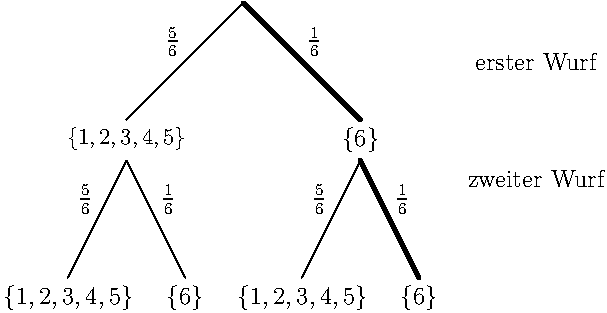
\includegraphics[width=10cm]{tree_intro_de}|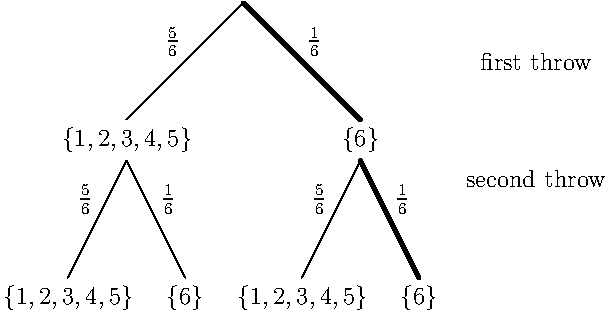
\includegraphics[width=10cm]{tree_intro_en}|
\end{center}

\tr|Der Pfad, der uns interessiert ist in diesem Diagramm fett gezeichnet. 
    Es gibt insgesamt $6\cdot 6 = 36$ mögliche Ausgänge dieses Experiments, aber nur einer davon ist \emph{günstig}.
    Die Wahrscheinlichkeit zweimal eine 6 zu würfeln isd deshalb:
   |The path we are interested in is highlighted in bold in the above tree diagram. 
    The first and the second time, there is just one case that we throw a 6. 
    So there is only one ($1\cdot 1$) favorable case (the case when we twice roll a 6). 
    The first and the second time there are 6 possible cases (the numbers 1,2,3,4,5 and 6), i.e. a total of $6\cdot 6 = 36$ cases. 
    The probability to roll a 6 twice is therefore|

\[
P(\text{\tr|zweimal ein |twice a | 6}) = \frac{1}{6}\cdot\frac{1}{6}=\frac{1}{36}
\]

\vspace{1cm}

\begin{ttile}{\tr|Erste Pfadregel|First Path Rule|}
\tr|In einem mehrstufigen Zufallsexperiment ist die Wahrscheinlichkeit eines einzelnen Pfades gleich dem Produkt der Wahrscheinlichkeiten 
    entlang dieses Pfades. 
   |In a multistep random experiment, the probability of a single path is equal to the product of the probabilities along that path.|
\end{ttile}
\vsp\vsp

\newpage
\tr|In einem Behälter sind 3 weisse und 5 schwarze Kugeln. Jemand zieht drei Kugeln, ohne sie zurückzulegen.
    Wie gross ist die Wahrscheinlichkeit, dass genau 2 weisse Kugeln (und damit auch genau eine schwarze) gezogen wurden?
   |There are 3 white and 5 black balls in a jar. Somebody draws three balls one after the other without putting them back. 
    What is the probability for exactly two white balls (and therefore exactly one black ball)?|
\begin{center}
\tr|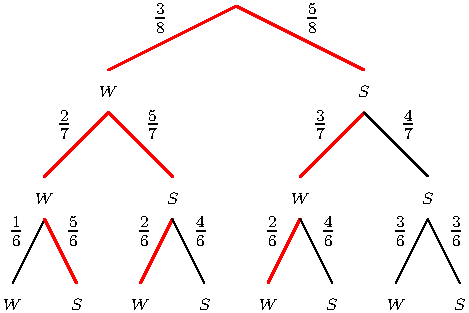
\includegraphics[width=12cm]{tree3_de}|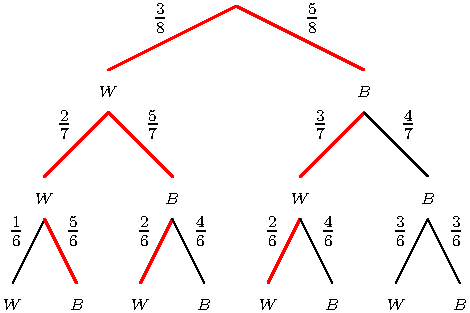
\includegraphics[width=12cm]{tree3_en}|
\end{center}

\tr|Nur die drei roten Pfade sind möglich.  
   |Only three paths are possible (highlighted in red). |
%The three results are mutually exclusive, meaning that each individual result contributes to the overall probability and each individual result increases the likelihood because another possibility is added. Therefore:
\ifEN
\begin{eqnarray*}
P(WWB\cup WBW \cup BWW ) &=& P(WWB)+ P(WBW)+ P(BWW)|\\
&=&\frac{3}{8}\cdot\frac{2}{7}\cdot\frac{5}{6}+\frac{3}{8}\cdot\frac{5}{7}\cdot\frac{2}{6}+\frac{5}{8}\cdot\frac{3}{7}\cdot\frac{2}{6}=\frac{15}{56}\approx 26.8\%
\end{eqnarray*}
\else
\begin{eqnarray*}
P(WWS\cup WSW \cup SWW ) &=& P(WWS)+ P(WSW)+ P(SWW)\\
&=&\frac{3}{8}\cdot\frac{2}{7}\cdot\frac{5}{6}+\frac{3}{8}\cdot\frac{5}{7}\cdot\frac{2}{6}+\frac{5}{8}\cdot\frac{3}{7}\cdot\frac{2}{6}=\frac{15}{56}\approx 26.8\%
\end{eqnarray*}
\fi
\vsp\vsp

\begin{ttile}{\tr|Zweite Pfadregel|Second Path Rule|}
\tr|In einem mehrstufigen Zufallsexperiment ist die  Wahrscheinlichkeit für das Auftreten von mehreren Pfaden gleich der Summe der Wahrscheinlichkeiten der 
    einzelnen Pfade.
   |In a multistep random experiment, the probability of multiple paths occurring is equal to the sum of the probabilities of each path. |
\end{ttile}
\vsp\vsp
\newpage
\begin{xxwrap}
\begin{exc}
\tr|Eine Münze wird dreimal geworfen. Wie gross ist die Wahrscheinlichkeit, dass 
   |A coin is flipped three times. What is the probability that|
\begin{enumerate}
\item \tr|nie \emph{Kopf} erscheint?|no \emph{head} occurs?|
\item \tr|genau einmal \emph{Kopf} erscheint?|exactly one \emph{head} occurs?|
\item \tr|genau zweimal \emph{Kopf} erscheint?|exactly two \emph{heads} occur?|
\item \tr|mindestens zweimal \emph{Kopf} erscheint?|at least two \emph{heads} occur?|
\end{enumerate}
\end{exc}
  \begin{Answer}
    \begin{enumerate}
    \item $\left(\frac12\right)^3$
    \item $3\cdot\frac18$
    \item $\frac38$
    \item $\frac38+\frac18=\frac12$
    \end{enumerate}
  \end{Answer}
\answerline{12}
\end{xxwrap}
\vfill
\begin{xxwrap}
\begin{exc}
\tr|Wir legen 7 (nicht unterscheidbare) Haselnüsse in 3 Teller mit den Farben Rot, Grün und Blau. Wie gross ist die 
    Wahrscheinlichkeit, dass
   |We put seven (indistinguishable) hazelnuts in three plates which are colored red, green and blue. What is the probability that |
\begin{enumerate}
\item \tr|Sie alle im roten Teller landen.|They land all in the red plate.|
\item \tr|Sie alle im gleichen Teller landen.|They land all in the same plate.|
\item \tr|Der blaue Teller leer bleibt.|The blue plate remains empty.|
\item \tr|Genau ein Teller leer bleibt.|Exactly one plate remains empty.|
\item \tr|Mindestens ein Teller bleibt leer.|At least one plate remains empty.|
\item \tr|Mindestens eine Haselnuss in jedem Teller landet.|At least one hazelnut lands in each plate.|
\end{enumerate}
\end{exc}
\begin{Answer}
  \begin{center}
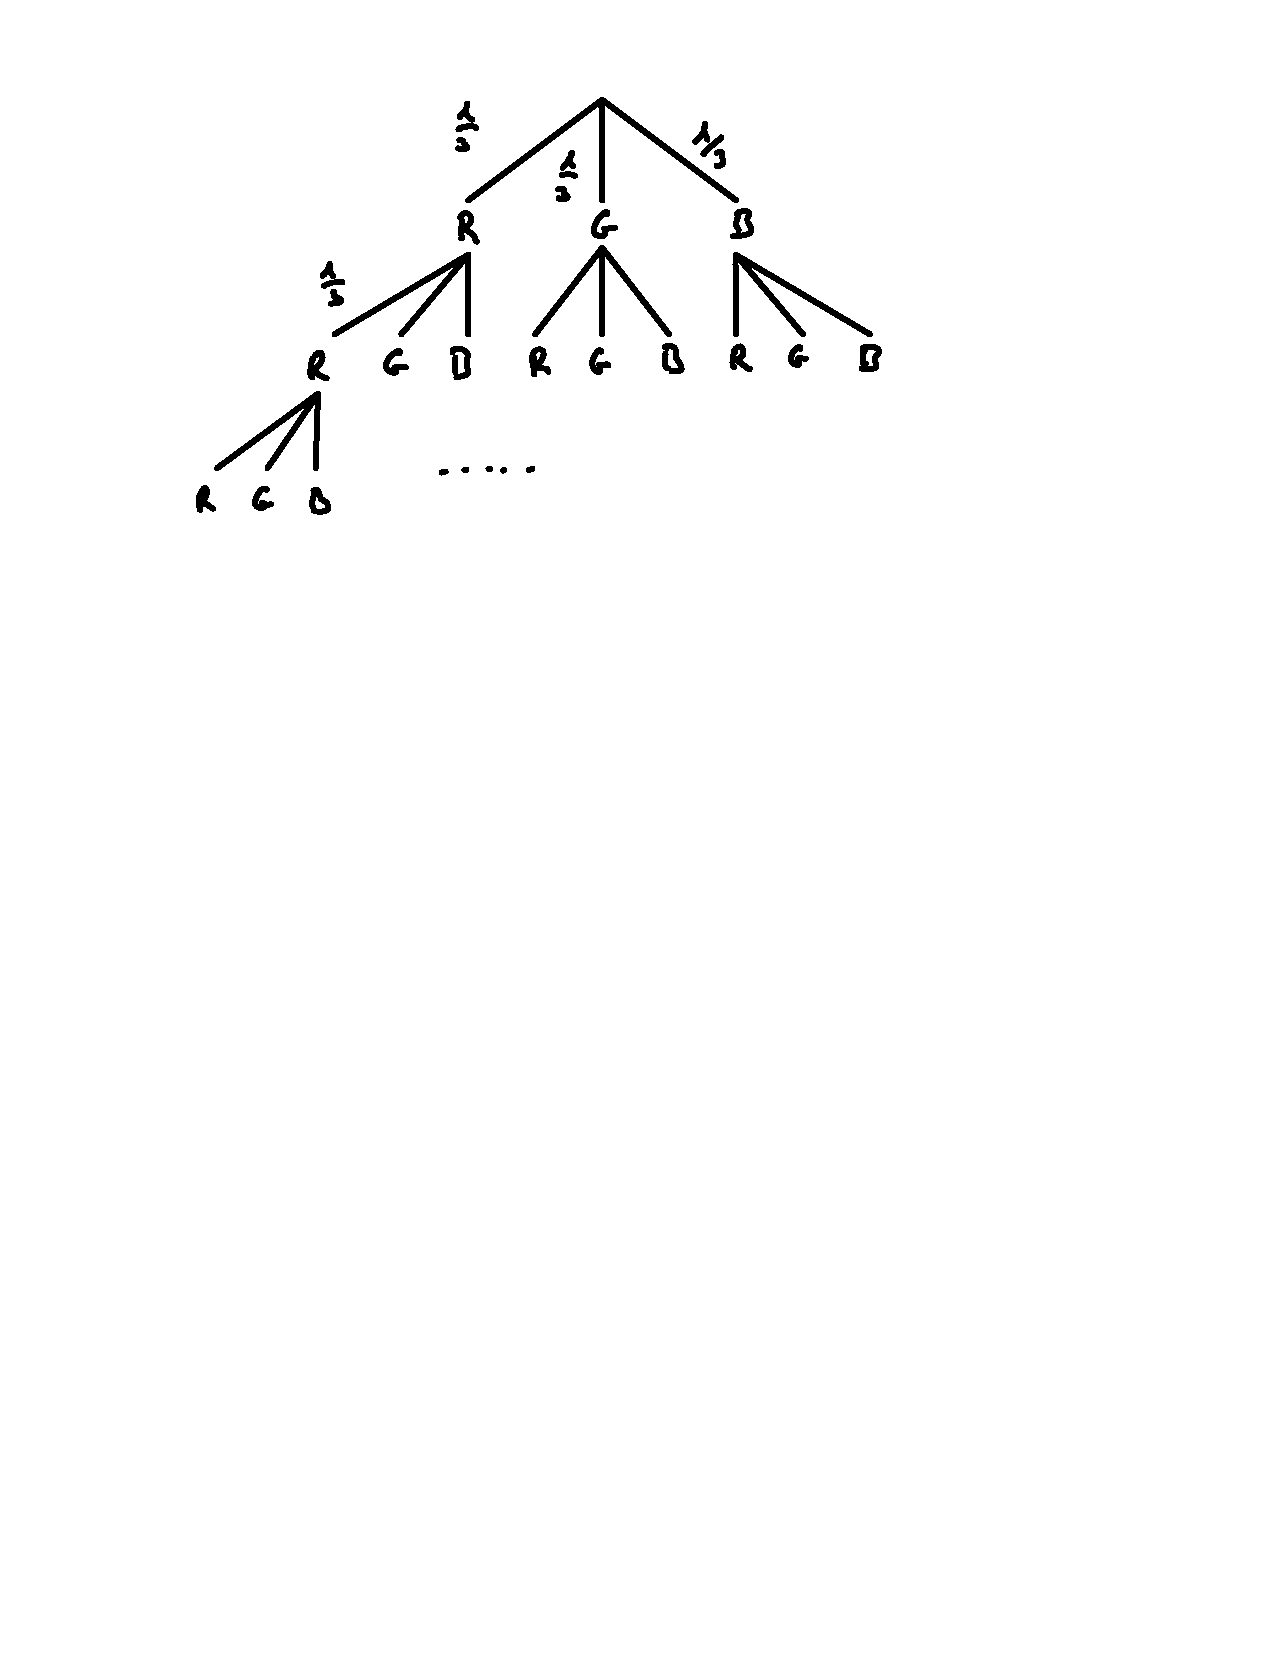
\includegraphics[width=0.5\textwidth]{images/probability/SOL_Nuts.pdf}
\end{center}
  \tr|Wenn man sich auf den Standpunkt stellt, dass die Tellerfarben gewählt werden (statt der Nüsse), so sieht man, 
      dass es sich hier um eine ungeordnete Stichprobe mit Zurücklegen handelt, aber wir kommmen auch ohne die 
      entsprechende Formel aus der Kombinatorik zurecht: 
     |If you take the point of view that we choose the colors of the plates instead of the hazelnuts,
     then this is unordered selection with repetition, but we can get away without the corresponding
     formula from combinatorics:|
  \begin{enumerate}
  \item $P(\text{\tr|alle rot|all red|})=\left(\frac13\right)^7= 0.0005$
  \item $P(\text{\tr|alle die gleiche Farbe|all the same color|})
         =P(\text{\tr|alle rot|all red|})+
         P(\text{\tr|alle grün|all green|})+
         P(\text{\tr|alle blau|all blue|})
         = 3\cdot\left(\frac13\right)^7=0.0014$
  \item $P(\text{\tr|blau leer|blue empty|})=\left(\frac23\right)^7= 0.0585$
  \item $P(\text{\tr|genau ein T. leer|exactly one plate empty|})$ \tr|ist \textbf{nicht} |ist \textbf{not} |
      $$P(\text{\tr|rot leer|red empty|})+P(\text{\tr|grün leer|green empty|})+P(\text{\tr|blau leer|blue empty|})=3\cdot P(\text{\tr|blau leer|blue empty|}$$
     \tr|weil die 3 entprechenden Mengen nicht diskjunkt sind. Aber |because these 3 set are not disjoint. But  |
      $$
      P(\text{\tr|genau ein T. leer|exactly one plate empty|})=3\cdot P(\text{\tr|genau blau leer|exactly blue plate empty|})
      $$   
      \begin{center}
      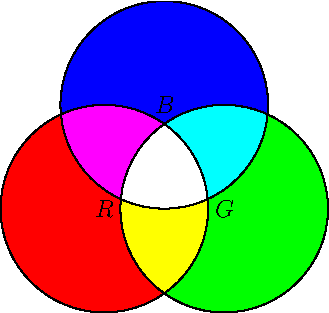
\includegraphics[width=4cm]{images/probability/plates.pdf}
    \end{center}
      \begin{align*}
        P(\text{\tr|genau blau leer|exactly blue plate empty|})&=P(\text{$B$ \tr|leer|empty|})\\ 
                                                               &\quad- P(\text{$B+G$ \tr|leer|empty|})\\
                                                               &\quad- P(\text{$B+R$ \tr|leer|empty|})\\
                                                               &\quad+P(\text{$B+G+R$ \tr|leer|empty|})\\
                                                               &=P(\text{$B$ \tr|leer|empty|})\\ 
                                                               &\quad -P(\text{\tr|alle in |all in|  $R$})\\ 
                                                               &\quad -P(\text{\tr|alle in |all in|  $G$})\\
                                                               &\quad+ 0\\
                                                               &=\circled{c}-2\cdot\circled{a}
      \end{align*}
      $$
      P(\text{\tr|genau ein T. leer|exactly one plate empty|})
      = 3\cdot\left( \circled{c}-2\cdot \circled{a}\right)=0.1756
      $$
    \item
      \begin{align*}
        P(\text{\tr|mindestens 1 leer|at least 1 empty|})
        &=P(\text{\tr| genau 1 leer|exactly 1 empty|})\\
        &\quad +P(\text{\tr| genau 2 leer|exactly 2 empty|})\\
        &\quad +P(\text{\tr| genau 3 leer|exactly 3 empty|})\\
        &=P(\text{\tr|genau 1 leer|exactly 1 empty|})\\
        &\quad +P(\text{\tr|alle in einem|all in one|})\\
        &\quad +0\\\
        &= \circled{d}+\circled{b}=0.1770
      \end{align*}
    \item $1-\circled{e}=0.8230$
  \end{enumerate}

\end{Answer}
\answerline{12}
\end{xxwrap}

\begin{xxwrap}
\begin{exc}
\tr|Lea und Bea haben je zwei Steine und werfen sie abwechselnd auf eine Blechdose. 
    Ihre Treffgenauigkeit ist jeweils $\frac{1}{3}$ und $\frac{1}{4}$. 
   |Lea and Bea each have two stones. They throw alternately at a tin can. Their accuracy is $\frac{1}{3}$ and $\frac{1}{4}$. |
\begin{enumerate}
\item \tr|Wie gross ist die Wahrscheinlichkeit, dass Lea als erste trifft, wenn sie beginnt?
         |What is the probability that Lea will be the first to hit when she starts?|
\item \tr|Wie gross ist die Wahrscheinlichkeit, dass Bea als erste trifft, wenn Lea beginnt?
         |What is the probability that Bea will be the first to hit when Lea starts?|
\item \tr|Und was ändert sich, wenn beide ihre Steine mehrmals verwenden können?
         |What if they have as many stones as necessary till one of them hits the can?|
\end{enumerate}
\end{exc}
\begin{Answer}
  \begin{center}
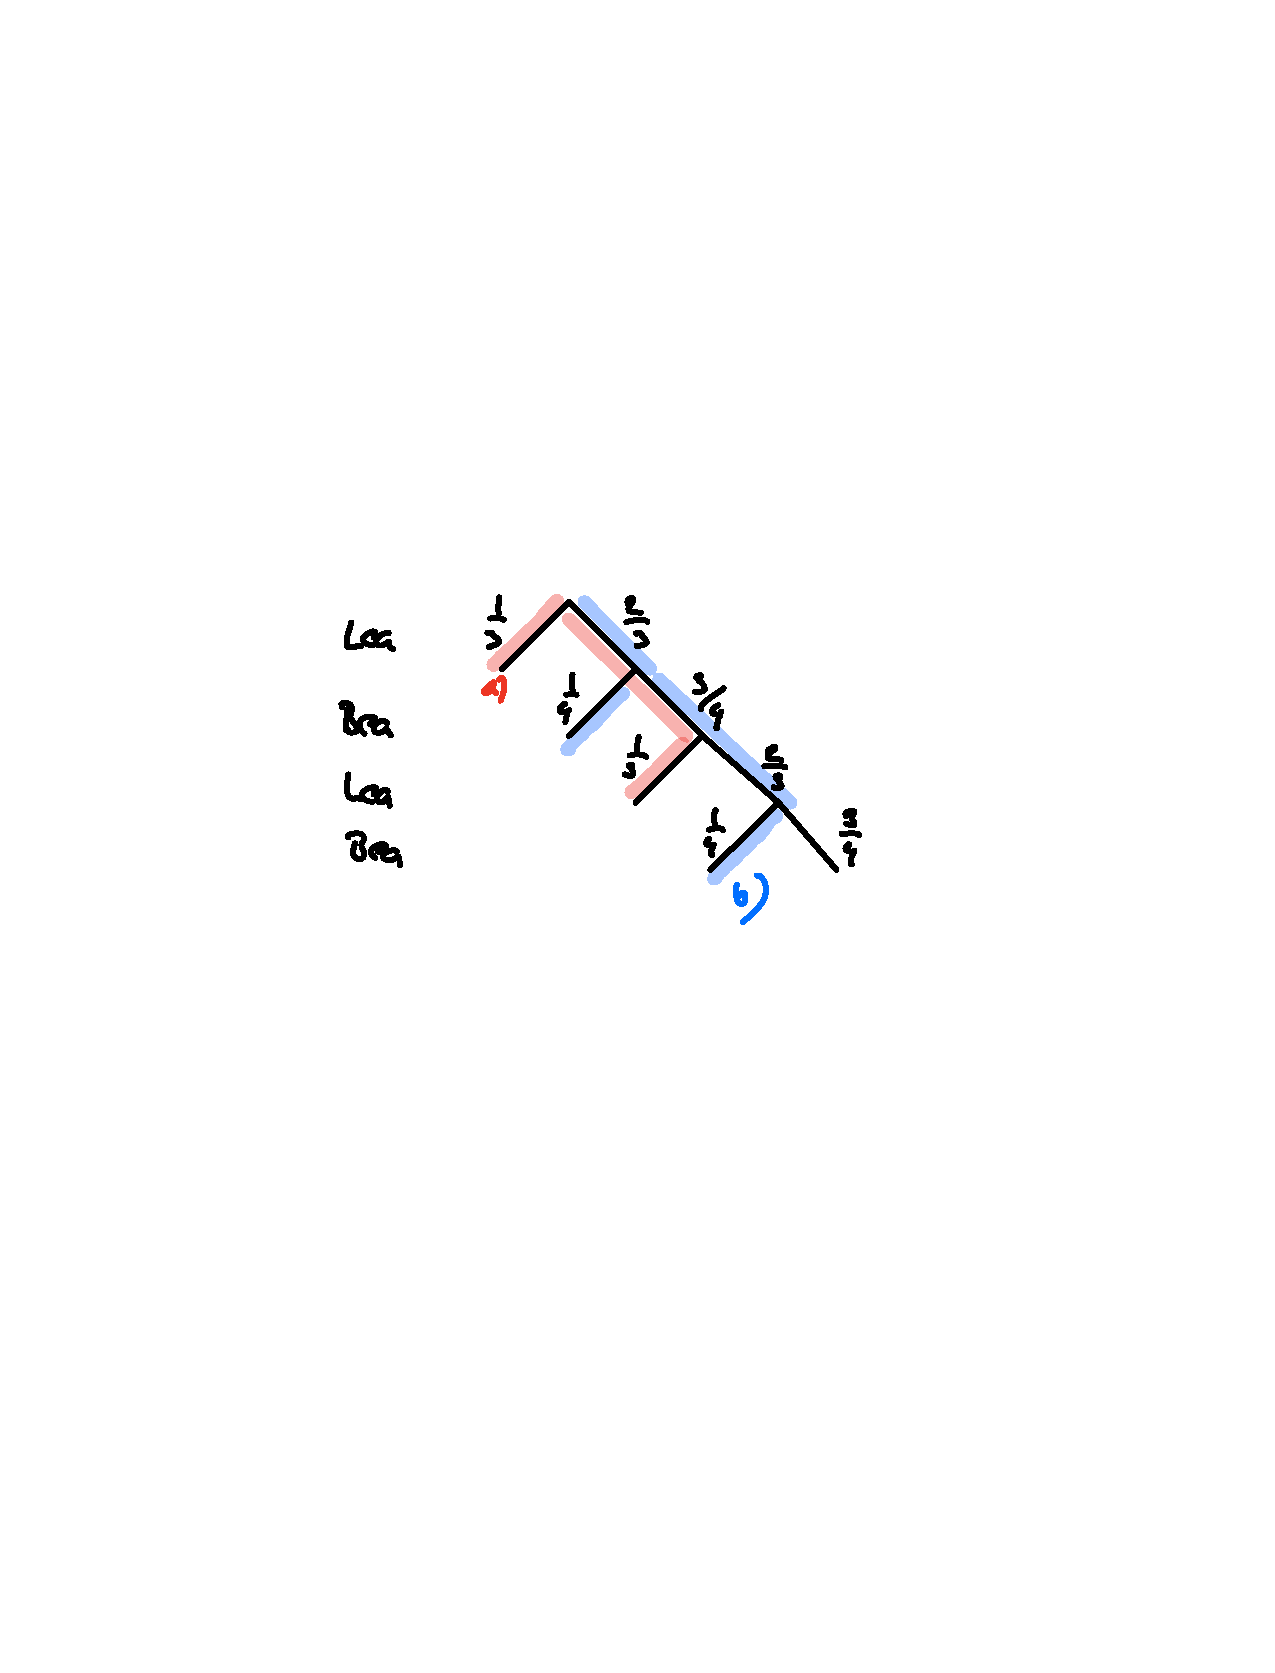
\includegraphics[width=0.5\textwidth]{images/probability/SOL_Stones.pdf}
\end{center}
  \begin{enumerate}
  \item $\frac13+\frac23\cdot \frac34\cdot\frac13=\frac12$
  \item $\frac23\cdot\frac14+\frac23\cdot\frac34\cdot\frac23\cdot\frac14=\frac14$
  \item 
    \begin{align*}
      P(\text{Lea \tr|gewinnt|wins|})&= \sum_{k=0}^\infty \left(\frac23\cdot\frac34\right)^k\cdot \frac13
                                       =\frac13\sum_{k=0}^\infty\left(\frac12\right)^k\\
                                     &=\frac13\cdot\frac1{1-\frac12}=\frac23\\
      P(\text{Bea \tr|gewinnt|wins|})&= 1-\frac23=\frac13
    \end{align*}
  \end{enumerate}
\end{Answer}
\answerline{12}
\end{xxwrap}


\begin{xxwrap}
\begin{exc}
\tr|Von einem Medikament ist bekannt, dass es mit einer Wahrscheinlichkeit von 80\% eine bestimmte Krankheit heilt. 
    Drei Patienten, die an dieser Krankheit leiden werden mit diesem Medikament behandelt. 
   |A drug is known to have a 80\% chance of success in the treatment of a disease. It is used to treat three patients suffering from this disease.|
\begin{enumerate}
\item \tr|Mit welcher Wahrscheinlichkeit werden alle drei Patienten geheilt?
         |What is the probability that all three patients will be cured?|
\item 
    \tr|Mit welcher Wahrscheinlichkeit werden mindestens zwei Patienten geheilt?
       |What is the probability that at least two patients will be cured?|
\end{enumerate}
\end{exc}
\begin{Answer}
  \begin{enumerate}
  \item $0.8^3$
  \item $0.8^3+3\cdot 0.8^2\cdot 0.2$
  \end{enumerate}
\end{Answer}
\answerline{12}
\end{xxwrap}

\begin{xxwrap}
\begin{exc}
    \begin{enumerate}
    \item \tr|Ein Würfel wird 7 mal geeworfen. Mit welcher Wahrscheinlichkeit wird mindestens einmal eine 5 oder eine 6 erscheinen? 
  |A die is thrown seven times. With which probability will one of the numbers 5 or 6 appear at least once?| 
\item
    \tr|Wie oft muss man den Würfel höchstens werfen so dass die Wahrscheinlichkeit, mindestens einmal eine 5 oder 6  zu würfeln  grösser als 99.5\% ist?
    |At least how many times would the die have to be thrown so that one of the numbers 5 or 6 is shown at least once with a  probability of 99.5\% or bigger?|
  \end{enumerate}
  \end{exc}
  \begin{Answer}
    \begin{enumerate}
    \item $1-P(\text{\tr|nie 5 oder 6|never 5 or 6|})=1-\left(\frac46\right)^7=0.941$
    \item $1-\left(\frac23\right)^n=0.995\Rightarrow n=13.067$ \tr|also 14 mal. |hence 14 times.| 
    \end{enumerate}
  \end{Answer}
\answerline{12}
\end{xxwrap}
\newpage
% Multistep random experiment:8 ends here

% [[file:../scripts.org::*Conditional probability][Conditional probability:8]]
\section{\tr|Bedingte Wahrscheinlichkeit|Conditional Probability|}\label{cond}

\begin{itemize}
\item
  \tr|Ein HIV Test hat eine \textbf{Sensitivität} von 99.8\%.
  Dies ist die Wahrscheinlichkeit, dass jemand, der HIV-positiv ist auch positiv getestet wird. 
  |An HIV test has a \textbf{sensitivity} of 99.8\%.  
  This corresponds to the probability that someone who is HIV-positive is also measured positive. |
\item
  \tr|Der Test hat eine \textbf{Spezifität} von 99.7\%. 
  Die ist die Wahrscheinlichkeit, dass jemand der HIV-negativ ist auch negativ getest wird.
  |The test also has a \textbf{specificity} of 99.7\%. 
  This corresponds to the probability that someone who is HIV-negative is also measured negative.|
\item
  \tr|Wir wissen auch, dass etwa 0.1\% der Personen, die einen  HIV test machen tatsächlich HIV positiv sind. 
  |We also know that approximately 0.1\% of people who do the HIV test are indeed HIV positive.|
\end{itemize}

\vsp

\textbf{\tr|Wie gross ist die Wahrscheinlichkeit, dass jemand HIV positiv ist, wenn er ein positives Testresultat hat. 
  |What is the probability that someone is HIV-negative if he/she gets a positive test result?| }

\vsp
\tr|In solchen Fällen sprechen wir von \textbf{bedingter Wahrscheinlichkeit}: Wie gross ist eine Wahrscheinlichkeit 
\emph{unter der Bedingung}, dass das Testresultat positiv ist. 
|In such cases, we speak of a \textbf{conditional probability}: 
What is the probability \textit{under the condition} that the test result is positive?|
\vsp

\tr|Das Problem wird einfacher, wenn wir mit konkreten Zahlen arbeiten. 
|The question becomes a little easier when we present concrete figures. |
\begin{itemize}
\item \tr|Nehmen wir an, dass innnerhalb eines Jahres 5 Millionen
  HIV Test durchgeführt werde.  |Let us assume that five million
  HIV tests will be carried out in one year.|
\item \tr|Da 0.1\% der Bevölkerung HIV-positiv sind ergibt die
  $5000000 \cdot 0.001 = 5000$ HIV-positive Personen and 4995000
  HIV-negative Personen.  |Since 0.1\% are HIV-positive, this
  corresponds to $5000000 \cdot 0.001 = 5000$ HIV-positive people and
  4995000 HIV-negative people.|
\item \tr|Weil der HIV Test eine Sensitivität von $99.8\%$ erhalten
  von diesen 5000 HIV-positiven Personen |Since the HIV test has a
  sensitivity of $99.8\%$, out of the 5000 HIV-positive people|
  \[
    5000\cdot 0.998=4990
  \]
  \tr|einen positiven Test und deshalb 10 Personen einen negativen.
  |receive a positive and therefore 10 people a negative test
  result.|
\item \tr|Da der HIV-Test eine Spezifität von $99.7\%$ hat,
  erhalten von den 4995000 Personen |Since the HIV test has a
  specificity of $99.7\%$, out of the 4995000 people |
  \[
    4995000\cdot 0.997=4980015
  \]
  \tr|einen negativen Test, d.h. 14985 einen positiven.  |receive a
  negative, i.e. 14985 a positive test result.|
\end{itemize}
\tr|Insgesamt erhalten $14985+4990=19975$ Personen eine positiven Test.
Davon sind 14985 Personen HIV-negativ, d.h. 
|Altogether, $14985+4990=19975$ people get a positive test result. 
Of these, 14985 people are HIV-negative, i.e.|
\[
  P(\text{
    \tr|HIV-negativ unter der Bedingung, dass der Test positiv ist
    |HIV-negative under the condition that the test is positive|
  })
  = \frac{14985}{19975}\approx 75\%
\]
\vsp
\tr|Obwohl sowohl Spezifität als auch Sensitivität des Tests seht hoch sind, sind 75\% der positiven
Testresultate falsch.
Der Grund dafür ist, das nur sehr wenige Personen HIV-postiv sind und deshalb wird
eine sehr grosse Anzahl von Tests an HIV-negativen Personen durchgeführt.
|Although both the specificity and sensitivity of the test are very high,
in 75\% of the cases a positive result is false.
This is due to the fact that only a few people are HIV-positive
and therefore a very large number of tests are carried out on people who are HIV-negative.|
\newpage




\tr|Seinen $E$ und $F$ zwei beliebige Ereignisse.| Let $E$ and $F$ be two arbitrary events.|
\vsp

\begin{ttile}{\tr|Bedingte Wahrscheinlichkeit|Conditional Probability|}
  \trr;Wir bezeichnen mit $P(E|F)$ die bedingte Wahrscheinlichkeit für das Auftreten von $E$
  unter der Bedingung, dass $F$ auftritt:
  ;We denote by $P (E|F)$ the conditional probability for the occurrence of $E$
  under the condition that $F$ occurs:;
\[
P(E|F)=\frac{P(E\cap F)}{P(F)}
\]
\end{ttile}
\vsp


\begin{center}
  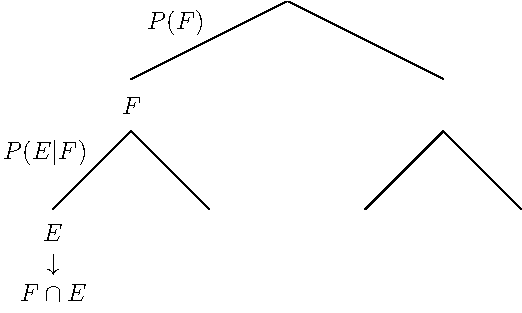
\includegraphics[width=9cm]{tree_Cond}
\end{center}


\trr;Im Falle von HIV sind wir deshalb an der Wahrscheinlichkkeit  $P(\text{HIV}- | \text{Test}+)$ interessiert, d.h. an der Wahrscheinlichkeit, dass eine Person HIV-negativ ist, wenn Sie einen
positiven Test erhalten hat. 
;In the HIV-case, we are therefore interested in the probability $P(\text{HIV}- | \text{test}+)$, 
i.e. the probability that someone is HIV negative under the condition that this person got a positive test result. Have a look at the following tree diagram:;

\begin{center}
  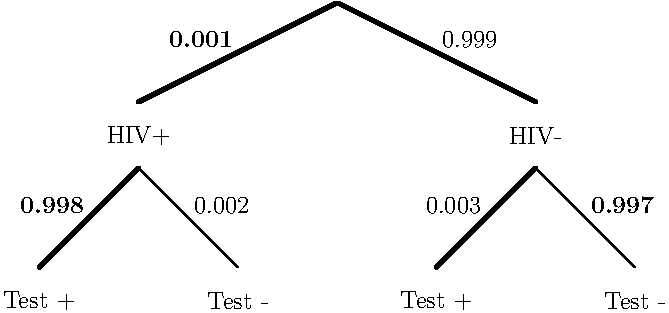
\includegraphics[width=9cm]{tree_HIV}
\end{center}

\tr|Die fettgedruckten Zahlen sind gegeben, die anderen können aus ihnen berechnet werden. 
Wir sind nur an den Fällen interessiert, in denen der Test positiv war, d.h. an den beiden fettgedruckten Pfaden. 
Die Wahrscheinlichkei für diese beiden Pfade ist $0.999\cdot 0.003 + 0.001\cdot 0.998$. Nun möchten wir wissen, wie wahrscheinlich der Pfad HIV-/Test+ (der die Wahrscheinlichkeit $0.999\cdot 0.003$ hat) 
in Bezug auf diese beiden Pfade ist.
|The bold numbers are given, the others may be calculated from them. Notice that we are only interested in the case when the test is positive, i.e. in the two bold paths. 
The chance that we have one of these two paths is $0.999\cdot 0.003 + 0.001\cdot 0.998$. 
We now want to know what the probability is that we get the path HIV-/test+ (with probability $0.999\cdot 0.003$) out of these two paths. 
Using number of favorable outcomes divided by number of possible outcomes we get|

\[
  P(\text{HIV}- | \text{Test}+)=\frac{0.999\cdot 0.003}{0.999\cdot 0.003 + 0.001\cdot 0.998}\approx 75\%
\]
\vsp

\begin{tile}
  \trr;Um die bedingt Wahrscheinlichkeit $P(E|F)$ zu berechnen zeichnet man ein Baumdiagramm, das sich zuerst bezüglich 
  $E$ aufspaltet und dann bezüglich $F$. Dann berechnet man die Wahrscheinlichkeit des Pfades der $E$ und $F$ erfüllt. 
  Diese Wahrscheinlichkeit teilt man durch die Wahrscheinlichkeit aller Pfade, die in $F$ enden. 
  ;Therefore, to calculate $P(E|F)$ we draw a tree diagram first differing in property $E$ and second in property $F$. 
  We then look for the path fulfilling $E$ and $F$ and calculate its probability. 
  We then divide this probability by the total probability of all paths which result in $F$. ;
\end{tile}



\tr|Die Verallgemeinerung des obigen Beislpiels führt auf den \emph{Satz von Bayes}. Schauen wir uns also den allgemeinen Fall an:
|This was an example of the \emph{Bayes' Theorem}. Let's have a look at the general case starting with the following tree diagram:|

\begin{center}
  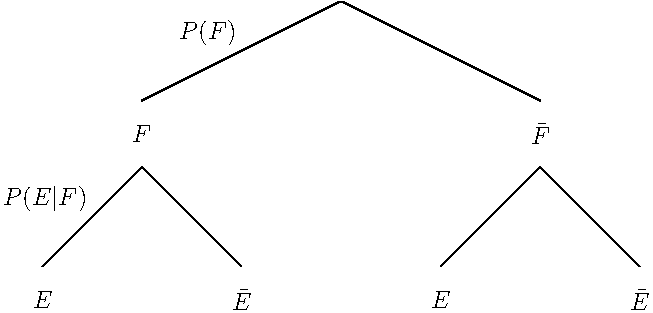
\includegraphics[width=7cm]{tree_Bayes_1}
\end{center}
\trr;Und es gilt; Therefore,; $P(E\cap F) = P(F) \cdot P(E|F)$.
\vsp

\tr|Wenn wir den obigen Baum umkehren erhalten wir|If we reverse the tree from above, we get|

\begin{center}
  \includegraphics[width=7cm]{tree_Bayes_2}
\end{center}

\trr;Und es gilt: ;Therefore, ;$P(E\cap F) = P(E) \cdot P(F|E)$. \tr|Zusammen mit dem vorigen Resultat|Thus,|
\[
  P(F) \cdot P(E|F)=P(E) \cdot P(F|E).
\]
\trr;Auflösen nach $P(E|F)$ ergibt ;Solving for $P(E|F)$ results in;

\[
  P(E|F)=\frac{P(E)\cdot P(F|E)}{P(F)}
\]

\tr|Ausserdem gilt|Further,|
\[
  P(F)= P(F\cap E)+P(F\cap \bar{E})=P(E)\cdot P(F|E) + P(\bar{E})\cdot P(F|\bar{E})
\]
    \aside{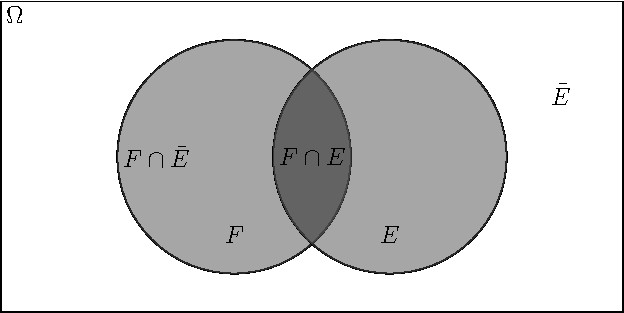
\includegraphics[width=4cm]{Bayes.pdf}}
\tr|Was zur folgenden Formel führt:|which leads to the following formula:|
\vsp

\begin{ttile}{\tr|Satz von Bayes|Bayes' Theorem|}
  \[
    P(E|F)=\frac{P(E)\cdot P(F|E)}{P(E)\cdot P(F|E) + P(\bar{E})\cdot P(F|\bar{E})}
  \]
\end{ttile}

\newpage
\tr|Wenn wir das HIV-Test Problem mit dieser Formel lösen, so erhalten wir für 
$E=\text{HIV-negativ}$ und $F=\text{Test positiv}$ 
|If we solve the HIV test problem with this formula, we get for $E=$HIV-negative and $F=$test positive|

\begin{eqnarray*}
  P(\text{HIV-} | \text{Test+}) &=& \frac{P(\text{HIV-})\cdot P(\text{Test+} | \text{HIV-})}{P(\text{Test+})}\\
                                &&\\
                                &=&\frac{P(\text{HIV-})\cdot P(\text{Test+ $|$ HIV-})}{P(\text{HIV-})\cdot P(\text{Test+ $|$ HIV-}) + P(\text{HIV+})\cdot P(\text{Test+ $|$ HIV+}) }
\end{eqnarray*}

\tr|Deshalb brauchen wir die folgenden Informationen:|Therefore, we need the following information:|

\begin{eqnarray*}
  P(\text{HIV+})&=&0.001\\
  P(\text{HIV-})&=&1-0.001=0.999\\
  P(\text{Test+$|$HIV-})&=&1-0.997=0.003\\
  P(\text{Test+$|$HIV+})&=&0.998
\end{eqnarray*}

\tr|Und der Satz von Bayes ergibt dann:| This results in|
\[
  P(\text{HIV-} | \text{Test+}) 
  =\frac{0.999\cdot 0.003}{0.999\cdot 0.003 + 0.001\cdot 0.998 }\approx 75\%
\]


\vfill
\newpage
\begin{xxwrap}
  \begin{exc}
    \tr|Rot-grün Farbenblindheit ist ziemlich einseitig verteilt. Jeder 12. Mann aber nur jede 288. Frau hat sie. Wie gross ist die Wahrscheinlichkeit, dass eine Person mit rot-grün Farbenblindheit 
    ein Mann ist?|
    Red-green color blindness is very one-sidedly distributed. Every 12th man, but only every 288th woman has it. What is the probability that a person who is red-green-blind is a man?|
  \end{exc}
  \begin{Answer}$\,$\\
    \begin{center}
    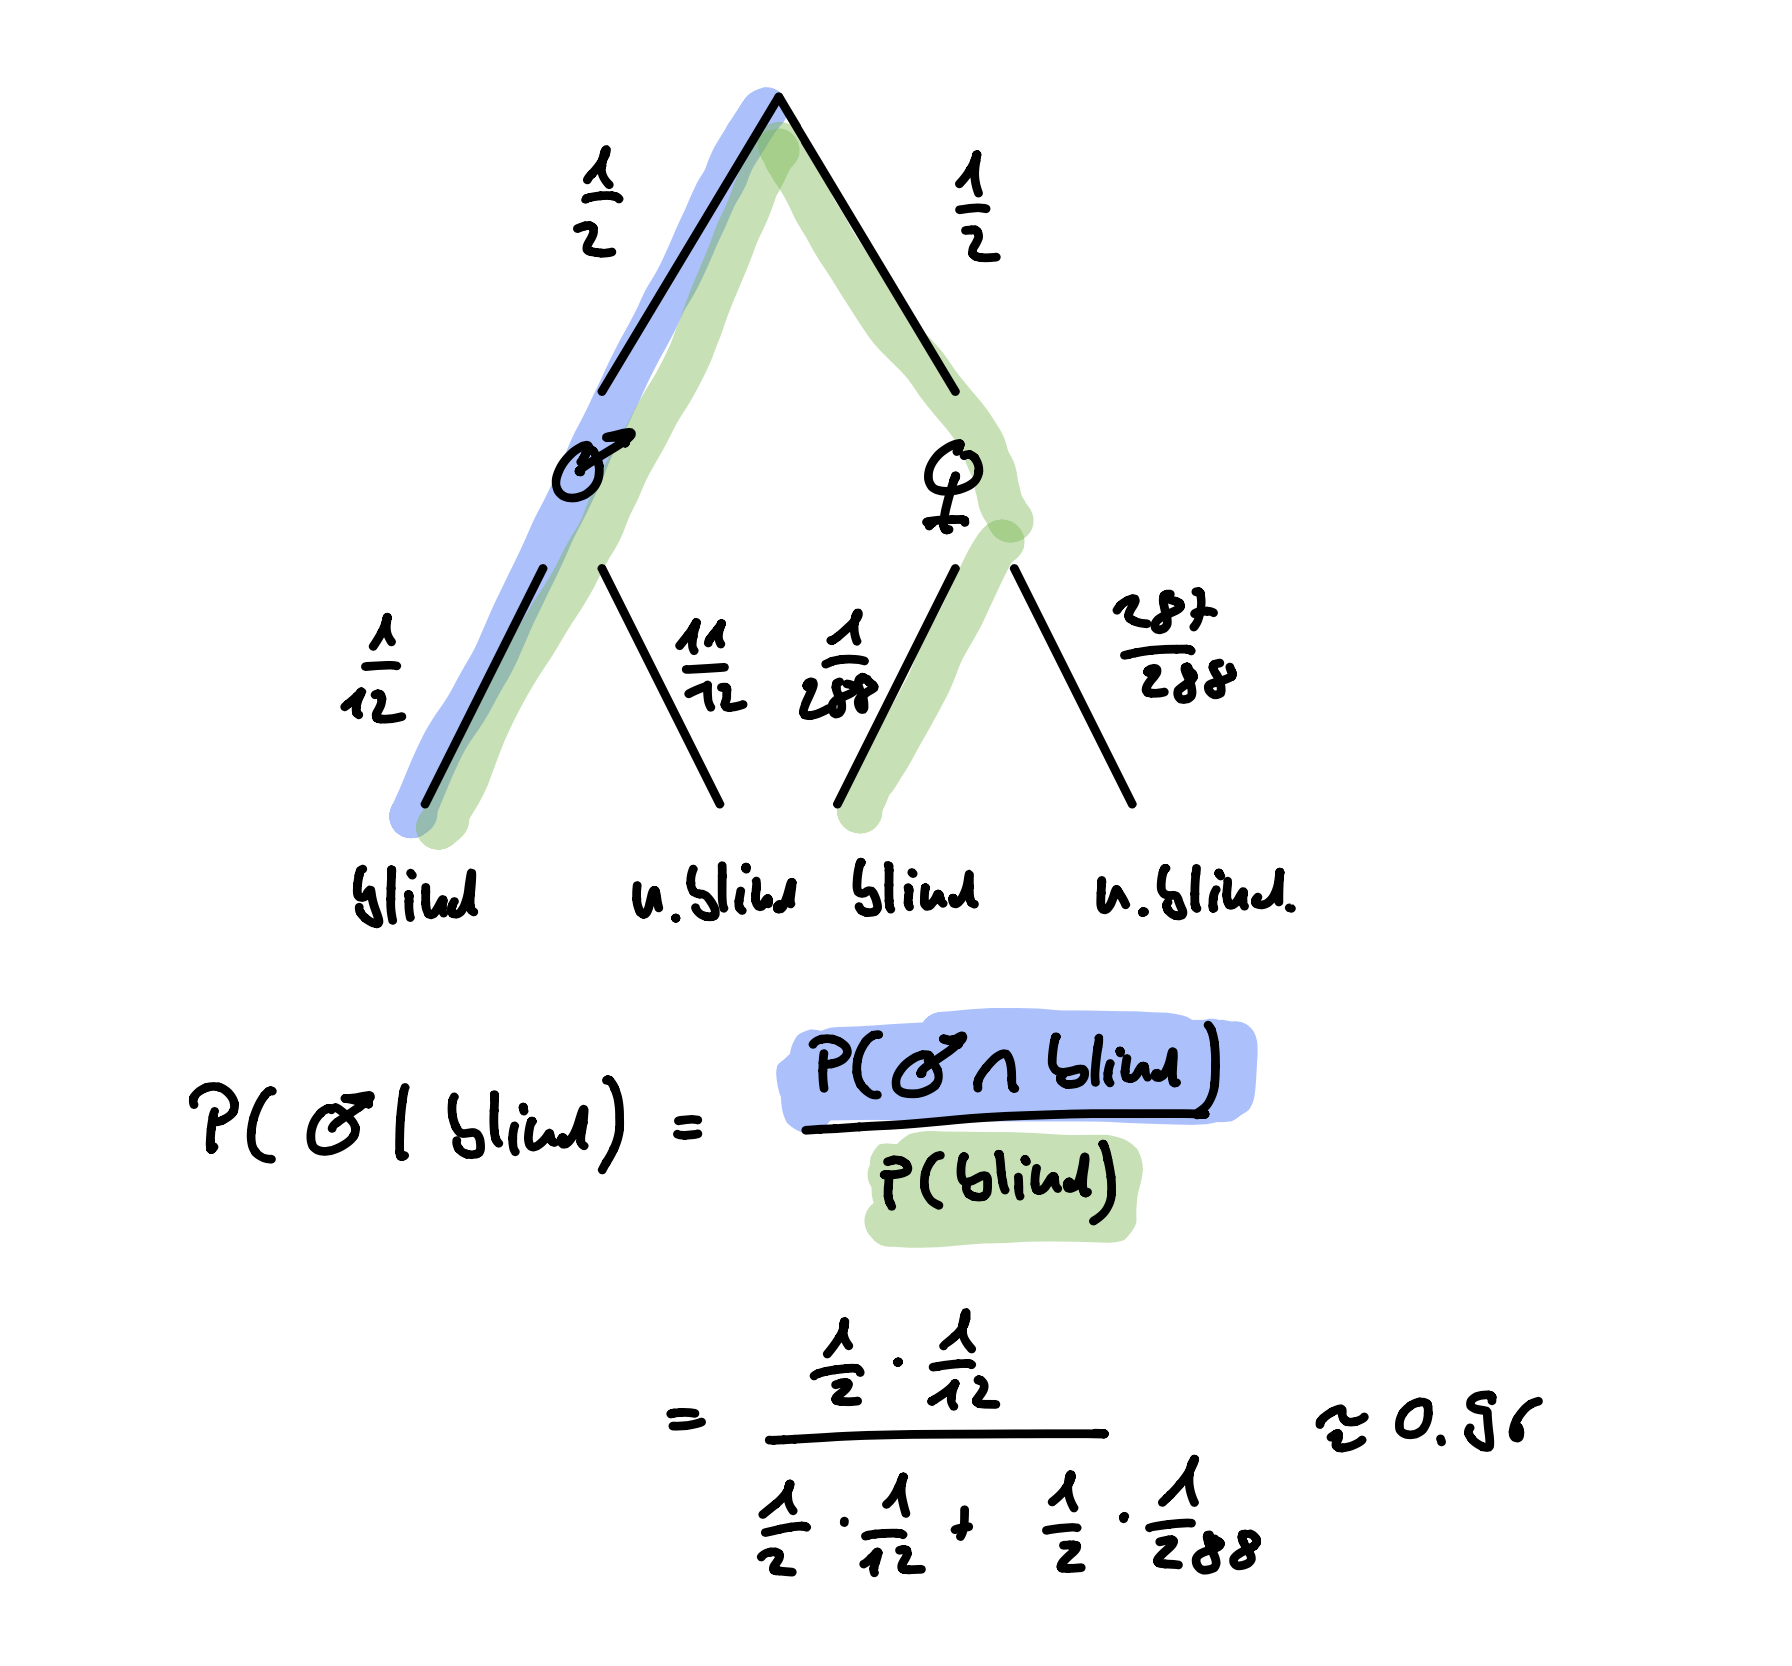
\includegraphics[width=8cm]{colorblind_SOL.png}
  \end{center}
  \end{Answer}
  \answerline{12}
\end{xxwrap}

\begin{xxwrap}
  \begin{exc}
    \tr|Eine Tasche enthält 14 rote und ein paar blaue Bälle. Zwei Bälle werden zusammen aus der Tasche genommen: Sie haben die gleiche Farbe. Wenn man nun schon weiss, 
       dass unter dieses Bedingung, die Wahrscheinlichkeit dafür, dass sie beide blau sind   $\frac{3}{16}$ ist, wie viele blaue Bälle sind  dann in der Tasche?
    |A bag contains fourteen red and a few blue balls. Two balls are drawn together; they are of the same color. 
    Under this condition, the probability is approximately $\frac{3}{16}$ that both balls are blue. How many blue balls are there in the bag?|
  \end{exc}
  \begin{Answer}$\,$\\
    \begin{center}
    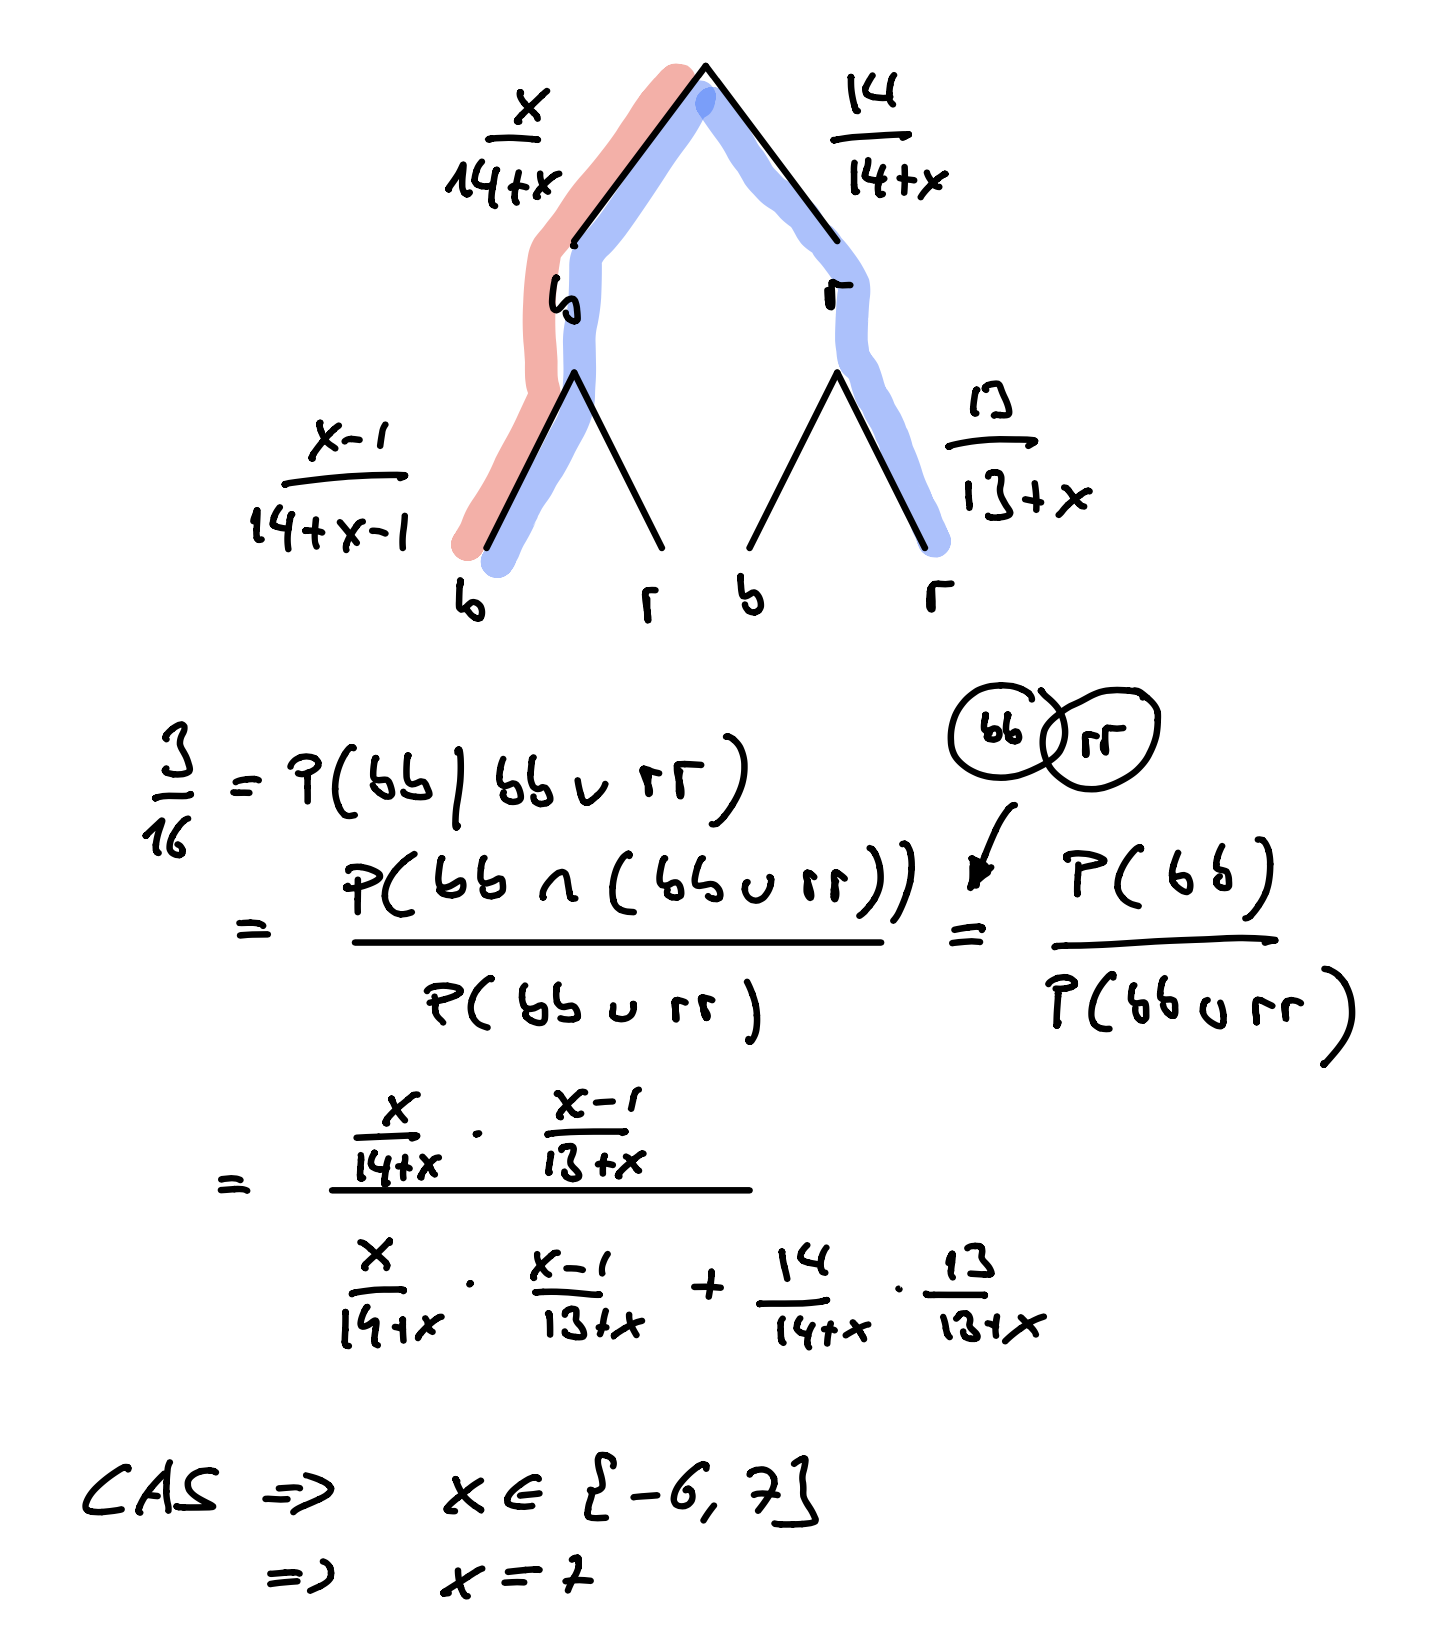
\includegraphics[width=8cm]{rbx_SOL1.png}\\
    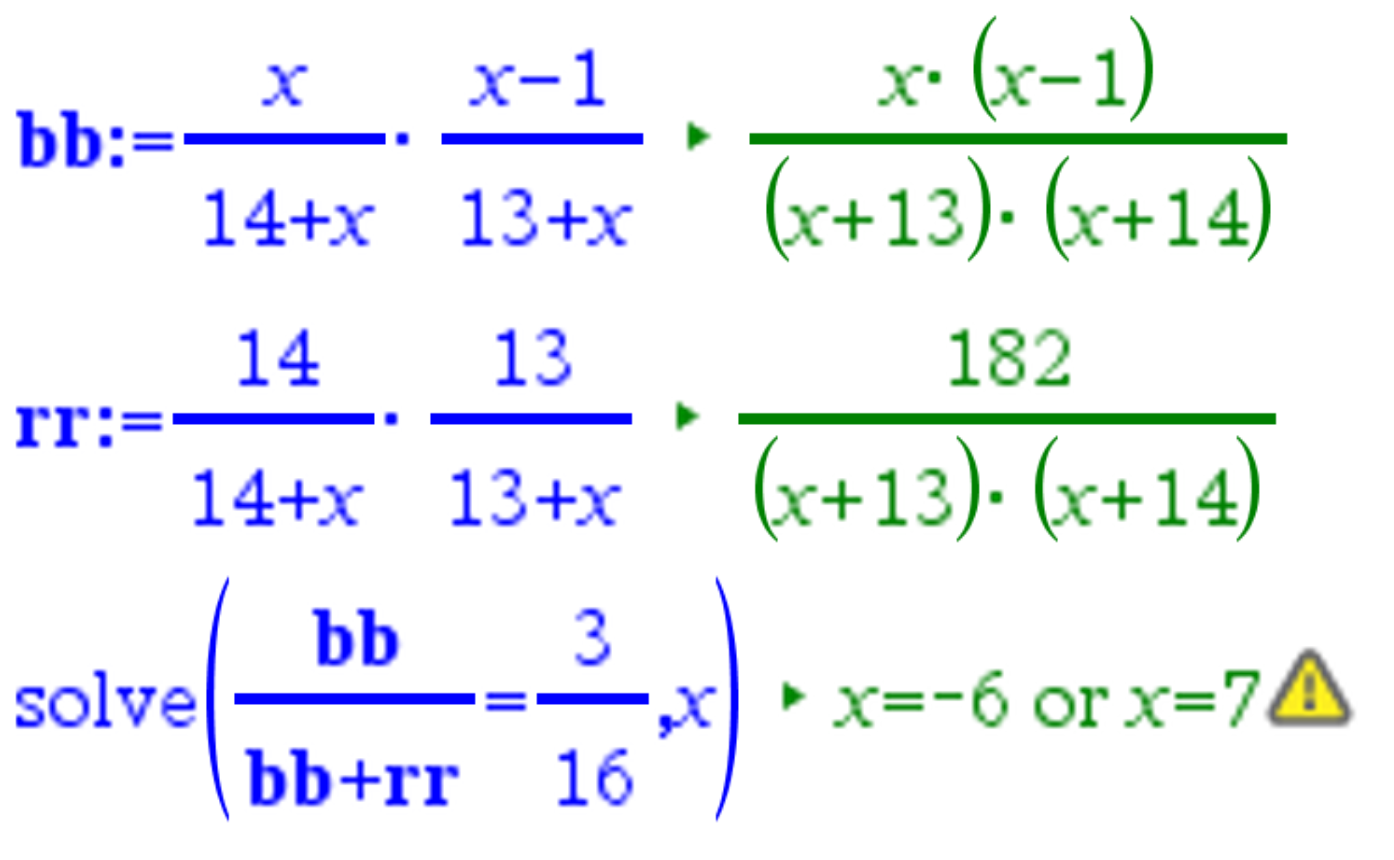
\includegraphics[width=4cm]{rbx_SOL2.png}\\
  \end{center}
  \end{Answer}
  \answerline{12}
\end{xxwrap}

% \begin{xxwrap}
%   \begin{exc}
%     \tr|Für einen Erwachsenen ist die Wahrscheinlichkeit, an Darmkrebs zu erkranken 0.3\%. Von den Erkrankten haben aber nur die Hälfte einen positiven Test, aber 3\% der Personen ohne Darmkrebs haben einen 
%     positvien Test. Wie gross ist die Wahrscheinlichkeit, dass eine Person mit einem positiven Test tatsächlich Darmkrebs hat. 
%     |The probability of an adult being diagnosed with colorectal cancer is 0.3\%. 
%     Of those with colorectal cancer, the test is positive in only half the cases, but 3\% of all people without colorectal cancer also get a positive result. 
%     What is the probability that a person with a positive test result has colorectal cancer?|
%   \end{exc}
%   \answerline{12}
% \end{xxwrap}

\begin{xxwrap}
  \begin{exc}

    \tr|Ob eine Person ein Magengeschwür entwickelt hängt stark von einem bestimmten Bakterium ab, das im Alter von 20 bis 40 recht häufig vorkommt. 
    Ein Test für dieses Bakterium (bekannt unter dem Namen  \emph{Helicobacter Pylor}) ist positiv bei 98\% aller Personen, die mit diesem Bakterium infiziert sind; der Test ist negativ bei 97\% der Personen, 
    die nicht infiziert sind. Die Wahrscheinlichkeit, dass eine Person mit positivem Test Resultat mit dem Bakterium infiziert ist 89\%. Welcher Anteil der 20 bis 40 jährigen ist mit dem Bakterium infiziert?
    |The development of stomach ulcers is strongly influenced by a certain bacterium, which is quite common in people aged 20 to 40. 
    A test for the detection of this bacterium (known as \emph{Helicobacter Pylori}) is positive in 98\% of people infected with this bacterium; it is negative in 97\% of uninfected people. 
    The probability that a person with a positive test result is infected with the bacterium is 89\%. What percentage of the group of people aged 20 to 40 are infected with the bacterium?|
  \end{exc}
  \begin{Answer}$\,$\\
    \begin{center}
    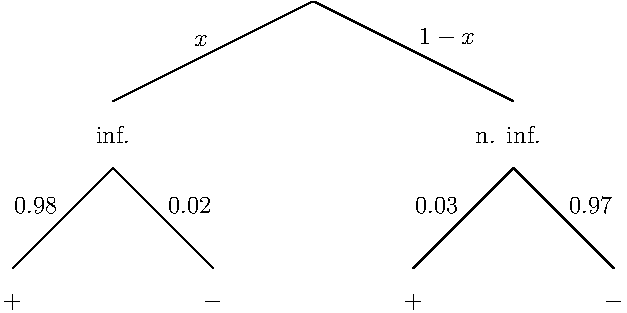
\includegraphics[width=8cm]{tree_bact_SOL_1.pdf}
  \end{center}
    \begin{align*}
      0.89&=P(\text{inf.}|+)=\frac{P(\text{inf.}\cap +)}{P(+)}\\
          &=\frac{x\cdot 0.98}{x\cdot 0.98+(1-x)\cdot 0.03}
    \end{align*}
    \[
      \overset{\text{CAS}}{\Rightarrow} x=0.199
    \]
  \end{Answer}
  \answerline{12}
\end{xxwrap}


\newpage
\begin{ttile}{\tr|Unabh"angige Ereignisse |Independent events|}
  \tr|Zwei Ereignisse $A$ und $B$ heissen \textbf{unabh"angig} falls gilt
  |Two events $A$ and $B$ are called \textbf{independent} if |
  \[
    P(A\cap B) = P(A)\cdot P(B)
  \]
\end{ttile}
\begin{xxwrap}
  \begin{exc}
    \tr|Zeigen Sie, dass die Unabh"angigkeit zweier Ereignisse $A$ und $B$
    gleichbedeutend ist mit
    |Show that independence of two events $A$ and $B$ is equivalent to |
    \[
      P(A|B)=P(A)\quad\text{\tr|wenn |if |$P(B)\neq 0$ }
    \]
    \tr|und |and | 
    \[
      P(B|A)=P(B)\quad\text{\tr|wenn |if |$P(A)\neq 0$ }
    \]
  \tr|Interpretieren Sie dieses Resulat. | Give an interpretation of this result.|
  \end{exc}
  \begin{Answer}
    \tr|Nehmen wir an, dass |Let's assume that| $P(B)\neq0$:
    \begin{align*}
      P(A|B)=P(A)&\Leftrightarrow \frac{P(A\cap B)}{P(B)}=P(A)\\
                 &\Leftrightarrow P(A\cap B)=P(A)P(B)
    \end{align*}
    \tr|Die Gleichung |The equation |
    \[
      P(A|B)=P(A)
    \]
    \tr|bedeutet, dass $B$ keinen Einfluss auf $A$ hat.|
        means that $B$ has no influence on $A$.|
  \end{Answer}
\answerline{10}
\end{xxwrap}

\begin{xxwrap}
  \begin{exc}
    \tr|Wir werfen eine M"unze dreimal. Seien $A$, $B$ und $C$ die folgenden Ereignisse:
    |We toss a coin three times. Let $A$, $B$ and $C$ be the following events:|
    \begin{align*}
      A&:=\text{\tr|1. Wurf ist \emph{Kopf}|First toss is \emph{head}|}\\
      B&:=\text{\tr|2. Wurf ist \emph{Kopf}|Second toss is \emph{head}|}\\
      C&:=\text{\tr|Genau zweimal \emph{Kopf} hintereinander|Exactly twice \emph{head} in a row|}
    \end{align*}
    \tr|Zeigen Sie | Show that|
    \begin{itemize}
    \item \tr|$A$ und $C$ sind unabh"angig.|$A$ and $C$ are independent.|
    \item \tr|$B$ und $C$ sind nicht unabh"angig.|$B$ and $C$ are not independent.|
    \end{itemize}
  \end{exc}
  \begin{Answer}
    \begin{align*}
      A&=\{\tr|K|H|**\} & P(A)=\frac12\\
      B&=\{*\tr|K|H|*\} & P(B)=\frac12\\
      C&=\{\tr|KKZ,ZKK|HHT,THH|\}& P(C)=\frac14
    \end{align*}
    \begin{align*}
      A\cap C&=\{\tr|KKZ|HHT|\} & P(A\cap C)=\frac18\\
      B\cap C&=\{\tr|KKZ,ZKK|HHT,THH|\}=C &  P(B\cap C)=\frac14
    \end{align*}
    \begin{align*}
      P(A\cap C)&=P(A)P(C)\\
      P(B\cap C)&\neq P(B)P(C)\\
    \end{align*}
\newpage
  \end{Answer}
\answerline{10}
\end{xxwrap}

\newpage
% Conditional probability:8 ends here

% [[file:../scripts.org::*Discrete Random Variables][Discrete Random Variables:1]]
\section{\tr|Diskrete Zufallsvariableln|Discrete Random Variables|}
\tr|Bis jetzt haben wir Ereignisse meist mit Worten umschrieben. Nun wollen wir diese Notation etwas kompakter gestalten
   |So far, we have described events mainly using words. It is far more convenient, where possible, to use numbers. |
\aside{\tr|Notation ist nicht der einzige Grund. Im nächsten Abschnitt werden Sie sehen, wie Zufallsvariabeln es uns erlauben, 
           ein Problem von der Ergebnismenge $\Omega$, in die reellen Zahlen $\R$ zu verschieben.
          |Well, notation is not the only reason. In the next section you will see how random variables allow us to push the problem
           from the sample space $\Omega$ to the real numbers $\R$.|}

\tr|Eine \textbf{Zufallsvariable} bildet die Ergebnisse eines Zufallsexperiments auf eine Zahl ab:
   |A \textbf{random variable} represents in number form the possible outcomes, which could occur for some random experiment:|
\vsp

\begin{ttile}{\tr|Zufallsvariable|Random variable|}
  \tr|Sei $\Omega$ eine Ergebnismenge. Eine Funktion $X: \Omega \to \mathbb{R}$ heisst eine
      \textbf{Zufallsvariable}. Sie bildet jedes Ergebnis auf eine auf eine reelle Zahl ab. 
     |Let $\Omega$ be a sample space. A function $X: \Omega \to \mathbb{R}$ is called a \textbf{random variable}. It maps each outcome of the sample space onto a real number.|
  \vsp

  \tr|Eine \textbf{diskrete} Zufallsvariable $X$ hat nur endlich oder abzählbar viele mögliche Werte.
     |A \textbf{discrete} random variable $X$ has only finitely or countably many  possible values.|
  \vsp

  \tr|Eine \textbf{stetige} Zufallsvariable $X$ hat als mögliche Werte ein Interval von reellen Zahlen.  
     |A \textbf{continous} random variable $X$ has a interval of real numbers as possible values. |
\end{ttile}
\vsp

\begin{example}
  \tr|Eine diskrete Zufallsvariable zählt meist etwas, wohingegen eine stetige Zufallsvariable etwas misst. Hier sind einige Beispiele: 
     |A discrete random variable involves a count whereas a continuous random variable involves measurements. Here are some examples:|
\vsp

\tr|Diskrete Zufalsvariabeln: |Discrete random variables:|
\begin{itemize}
\item \tr|Die Summe der Augen bei zwei Würfeln.|The sum of numbers of pips of two dice. |
\item
  \tr|Die Anzahl Fahrräder die in einem Laden jedes Jahr verkauft werden.
     |The number of new bicycles sold each year by a bicycle store.|
   \item
     \tr|Die Anzahl defekter Glühbirnen, in einer Sammelbestelllung.
        |The number of defective light bulbs in the purchase order of a city store.|
\end{itemize}

\tr|Stetige Zufallsvariabeln:| Continuous random variables:|
\begin{itemize}
\item
  \tr|Die Körpergrössen, einer Gruppe von Personen liegen  alle im Bereich $50<x<250$cm.
     |The heights of men could all lie in the interval $50<x<250$cm.|
   \item
     \tr|Das Wasservolumen in einem Regenwassertank in einem bestimmten Monat.
     |The volume of water in a rainwater tank during a given month.|
\end{itemize}

\end{example}

\vsp


\newpage
\begin{xxwrap}
\begin{exc}
\tr|in jedem der folgenden Beispiele |For each of the following|
\begin{itemize}
\item \tr|identifizieren Sie die Zufallsvariable, |identify the random variable being considered,|
\item \tr|geben Sie mögliche Werte der Zufallsvariabeln an, |give possible values for the random variable,|
\item \tr|geben Sie an, ob die Zufallsvariabel stetig oder diskret ist. |indicate whether the variable is continuous or discrete.|
\end{itemize}
\begin{enumerate}
\item \tr|Um die Regenmenge während 24 Stunden in Baden zu messen, wird die Wasserhöhe in einem Auffangbehälter (mit Höhe 200mm) verwendet. 
         |To measure the rainfall over a 24-hour period in Baden, the height of water collected in a rain gauge (up to 200 mm) is used.|
\item \tr|Um den Bremsweg eines Reifentyps zu untersuchen wird ein Bremsexperiment durchgeführt. 
         |To investigate the stopping distance for a tyre with a new tread pattern a braking experiment is carried out. |
\item \tr|Um die Zuverlässigkeit eines Lichtschalters zu testen, wird es so lange an und ausgeschalter, bis er nicht mehr funktioniert. 
         |To check the reliability of a new type of light switch, switches are repeatedly turned off and on until they fail.|
\end{enumerate}
\end{exc}
\begin{Answer}
  \begin{enumerate}
  \item 
    \begin{itemize}
    \item $X=\text{\tr|Wasserhöhe im Behälter|height of water in gauge|}$.
    \item \tr|Werte|Range| $=[0,200]$ 
    \item \tr|stetig|continuous|
    \end{itemize}
  \item 
    \begin{itemize}
    \item $X=\text{\tr|Länge des Bremsweges|length of breaking distance|}$.
    \item \tr|Werte|Range| $=[0,\infty]$ 
    \item \tr|stetig|continuous|
    \end{itemize}
  \item 
    \begin{itemize}
    \item $X=\text{\tr|Anzahl Umschaltungen bis zum Ausfall|number of uses until fail |}$.
    \item \tr|Werte|Range| $=1,2,3,\ldots$ 
    \item \tr|diskret|discrete|
    \end{itemize}
  \end{enumerate}
\end{Answer}
\answerline{12}
\end{xxwrap}
\vfill

\begin{xxwrap}
\begin{exc}
\tr|Ein Supermarkt hat vier Wagen $A$, $B$, $C$ und $D$. Die Leitung des Supermarktes überprüft nun die Wagen. 
Falls eine Wage funktioniert, so wird ein J notiert, andernfalls ein N. 
    Die Zufallsvariable $X$ sei die Anzahl funktionierender Wagen. 
   |A supermarket has four weighing devices $A,B,C$ and $D$. Management checks these devices. 
If a weighing device is accurate a yes (Y) is recorded; otherwise, no (N) is recorded.
    The random variable $X$ being considered is the number of weighing devices which are accurate. |
\begin{enumerate}
\item \tr|Welche Werte kann $X$ annehmen? |What values can $X$ have?|
\item \tr|Erstellen Sie eine Tabelle der möglichen Ergebnisse und der entsprechenden Wert von $X$. 
          Beschreiben Sie mit der Variabeln $X$, die Ereignisse \emph{zwei Wagen funktionieren} und \emph{mindestens zwei Wagen funktionieren}. 
         |Tabulate the possible outcomes and the corresponding values for $X$.
          Describe, using $X$, the events of two being accurate and of at least two being accurate.|
\end{enumerate}
\end{exc}
\begin{Answer}
  \begin{enumerate}
  \item $X\in\{0,1,2,3,4\}$
  \item
    \texttt{
    \renewcommand{\arraystretch}{0.7}
      \ifEN
      \begin{tabular}[t]{cccccc}
        &YYYY&YYYN&YYNN&YNNN&NNNN\\
        &    &YYNY&YNYN&NYNN&    \\      
        &    &YNYY&NYYN&NNYN&    \\
        &    &NYYY&YNNY&NNNY&    \\
        &    &    &NYNY&    &    \\
        &    &    &NNYY&    &    \\
        $X =$ & 4  &  3 & 2  &  1 &0    
      \end{tabular}
      \else
      \begin{tabular}[t]{cccccc}
        &JJJJ&JJJN&JJNN&JNNN&NNNN\\
        &    &JJNJ&JNJN&NJNN&    \\      
        &    &JNJJ&NJJN&NNJN&    \\
        &    &NJJJ&JNNJ&NNNJ&    \\
        &    &    &NJNJ&    &    \\
        &    &    &NNJJ&    &    \\
        $X =$ & 4  &  3 & 2  &  1 &0    
      \end{tabular}
      \fi
    }
    \begin{itemize}
    \item \tr|2 Wagen funktionieren|2 devices accurate|: $X=2$
    \item \tr|Mindestens 2 funktionieren|at least two accurate|: $X\in \{2,3,4\}$ 
    \end{itemize}
  \end{enumerate}
\end{Answer}
\answerline{12}
\end{xxwrap}
\vfill

\newpage
% Discrete Random Variables:1 ends here

% [[file:../scripts.org::*Discrete Probability Distributions][Discrete Probability Distributions:2]]
\section{\tr|Diskrete Wahrscheinlichkeitsverteilungen|Discrete Probability Distributions|}
\tr|Wir werfen zwei Würfel gleichzeitig. Der Ereignisraum $\Omega$ dieses Zufallsexperiments besteht aus allen Paaren von ganzen Zahlen zwischen 1 und 6, z.B. wären $(3,3)$ und $(2,5)$ solche Ergebnisse. 
    Eine mögliche Zufallsvariable wäre die Summe der Augenzahlen. Die möglichen Werte diese Zufalsvariable sind die natürlichen Zahlen zwischen 2 und 12. 
   |We throw two dice at the same time. The sample space $\Omega$ of this random experiment consists of all pairs of two integers between 1 and 6, i.e. $(2,5)$ and $(3,3)$ would be two examples of outcomes.
    A random variable is given by the sum of these pips. The values of this random variable are natural numbers between 2 and 12. |
\tr |Wir wollen untersuchen, mit welcher Wahrscheinlichkeit diese Zufallsvariable einen gewissen Wert annimmt. 
     Z.B. taucht der Wert 2 viel seltener auf als der Wert 7, da der Wert 2 nur dann erreicht wird, wenn wir mit beiden Würfeln eine 1 würfeln, den Wert 7 erreichen wir hingegen
     in den folgenden Fällen   $(1,6),(2,5),(3,4)$,$(4,3)$,$(5,2)$ und $(6,1)$, d.h. in 6 Fällen. 
    |We are now interested in the question with what probability a certain value is taken by the random variable.  
     The value 2 occurs much less frequently than the value 7, because the value 2 is only obtained if we roll a 1 with both dice.  
     The value 7 is obtained when we roll $(1,6),(2,5),(3,4)$,$(4,3)$,$(5,2)$ and $(6,1)$, i.e. in 6 cases. 
     If we map each value to its probability of occurrence, we get a new function:|
\vsp\vsp

\begin{ttile}{\tr|Wahrscheinlickeitsverteilung|Probability distribution|}
  \tr|Sei $X: \Omega\to\mathbb{R}$ eine diskrete Zufallsvariable, die die Werte $x_1, x_2, \ldots, x_n$ annimmt.
  Die Menge $\{\omega\in\Omega:\, X(\omega)=x_i\}$ (Abkürzung $\{X=x_i\}$), d.h. die Menge aller Ergebnisse, welcher die Zufallsvariable die Zahl $x_i$ zuordnet,
  hat eine gewisse Wahrscheinlichkeit, die von $x_i$ abhängt. 
  Nennen wir diese Wahrscheinlichkeit $F(x_i)$,
  die \textbf{Wahrscheinlichkeitsverteilung} (oder kurz \textbf{Verteilung})  von $X$.
  |Let $X: \Omega\to \mathbb{R}$ be a discrete random variable taking the values $x_1, x_2, \ldots, x_n$.
  The set $\{\omega\in\Omega:\, X(\omega)=x_i\}$ (shortcut $\{X=x_i\}$), i.e. the set of all outcomes to which the
  random variable assigns the number $x_i$ has a certain probability, depending on $x_i$.
  Let's call this probability $F(x_i)$. 
  The \textbf{probability distribution}   (or simply \textbf{distribution})  of $X$
  is the function 
  $F$ which  maps each value $x_i$ onto ``its probability'' $P(X=x_i)$.|
\end{ttile}
\vsp

\tr|In unserem Beispiel bedeutet dies: Insgesamt gibt es 36 Paare $(x,y)$ mit 
    $$x, y \in \{1,2,3,4,5,6\}$$. 
    Die Ausgensumme 2 kann nur mit dem Paar $(1,1)$ erreicht werden, d.h. die Wahrscheinlichkeit für den Wert 2 ist $\frac1{36}$. 
    Die restlichen Werte können in der folgenden Tabelle abgelesen werden:
   |In our example this means: In total there are 36 possible ordered pairs $(x,y)$ with $x, y \in \{1,2,3,4,5,6\}$. 
    The sum of pips 2 is only reached with $(1,1)$, i.e. the probability of the value 2 is equal to $\frac{1}{36}$. 
    The other values can be read off in the following table:|
\begin{center}
\begin{tabular}{c|c|c|c|c|c|c|c|c|c|c|c}
\tr|$X$-Werte|$X$-values| & 2 & 3 & 4 & 5 & 6 & 7 & 8 & 9 & 10 & 11 & 12 \\
\hline
$F(x_i)$ & $\frac{1}{36}$ & $\frac{2}{36}$ &$\frac{3}{36}$ &$\frac{4}{36}$ &$\frac{5}{36}$ &$\frac{6}{36}$ &$\frac{5}{36}$ &$\frac{4}{36}$ &$\frac{3}{36}$ &$\frac{2}{36}$ & $\frac{1}{36}$ 
\end{tabular}
\end{center}
\vsp

\begin{remark}
\tr|Die Summe aller $F(x_i)$-Werte ist natürlich genau 1. |The sum of all $F(x_i)$-values is of course just 1!|
\end{remark}


\begin{xxwrap}
\begin{exc}
\tr|Bestimmen Sie $k$ in den folgenden Verteilungen:
   |Find $k$ in these probability distributions:|
   \begin{enumerate}
   \item \begin{tabular}{|c|c|c|c|}
     $x_i$ & 0 & 1 & 2\\\hline $F(x_i)$ & 0.3 & $k$ & 0.5
   \end{tabular}
   \item \begin{tabular}{|c|c|c|c|c|}
     $x_i$ & 0 & 1 & 2 & 3\\\hline $F(x_i)$ & $k$ & $2k$ & $3k$ & $k$  
   \end{tabular}
 \end{enumerate}
\end{exc}
\begin{Answer}
  \begin{enumerate}
  \item $1=0.3+k+0.5\implies k=0.2$ 
  \item $1=k-2k+3k+k=1\implies 7k=1\implies k=\frac17$
  \end{enumerate}
\end{Answer}
\answerline{12}
\end{xxwrap}

\begin{xxwrap}
\begin{exc}
\tr|Wir werfen zwei Münzen und zählen die Anzahl \emph{Köpfe}. Geben Sie die zugehörige Zufallsvariable und ihre Verteilung an. 
   |We toss two coins and count the number of heads. Describe the random variable and its probability distribution. |
\end{exc}
\begin{Answer}$\,$
  \begin{center}
  \begin{tabular}[t]{|c|c|c|c|}
    $x_i$&2&1&0\\\hline
    $P(X=x_i)$&$\frac14$&$\frac12$&$\frac14$
  \end{tabular}
\end{center}
\end{Answer}
\answerline{20}
\end{xxwrap}

\begin{xxwrap}
\begin{exc}
\tr|Zeigen Sie, dass die folgenden Funktionen Wahrscheinlichkeitsverteilungen sind, d.h., dass $0\leq F(x_i)\leq 1$ für alle $x_i$ 
    und dass die Summe aller $F(x_i)$ gleich 1 ist. 
   |Show that the following are probability distribution functions, i.e. that $0\leq F(x_i)\leq 1$ for all $x_i$ 
    and the sum of all $F(x_i)$ equals 1. |
\begin{enumerate}
\item $F(x)=\frac{x^2+1}{34}$ for $x=1,2,3,4$
\item $F(x)=\binom{3}{x}\cdot 0.6^x\cdot 0.4^{3-x}$ for $x=0,1,2,3$
\end{enumerate}
\end{exc}
\begin{Answer}
  \begin{center}
   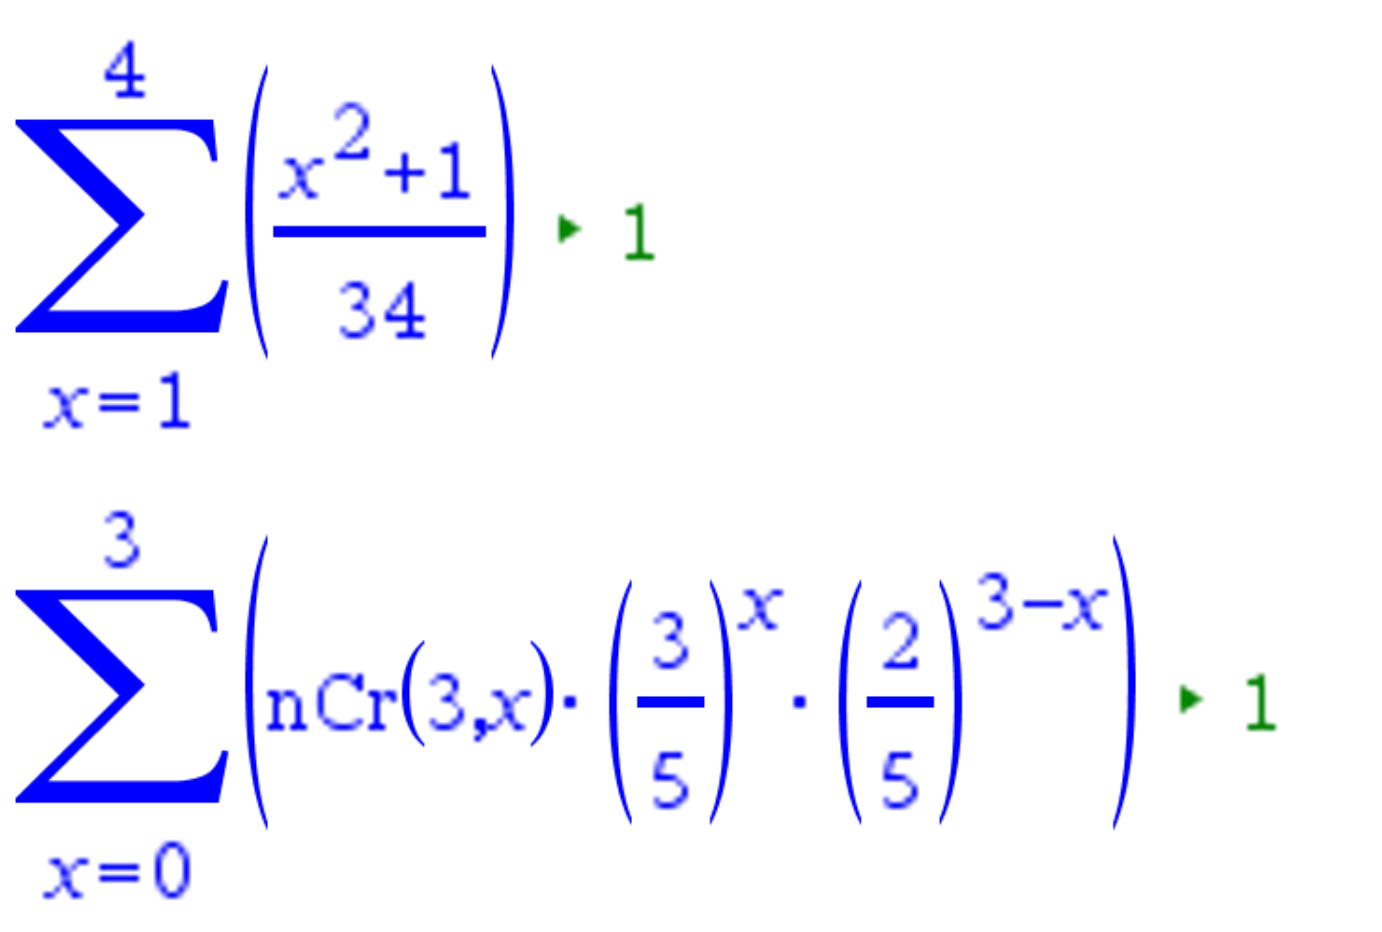
\includegraphics[width=6cm]{SOL_dist_01.png} 
  \end{center}
\end{Answer}
\end{xxwrap}
\answerline{12}
\vfill

\begin{xxwrap}
\begin{exc}
\tr|Ein Beutel enthält 4 rote und 2 blaue Murmeln. 2 Murmeln werden (ohne Zurücklegen) zufällig ausgewählt. Sei $X$ die Anzahl roter Murmeln unter den Ausgewählten. 
    Bestimmen Sie die Wahrscheinlichkeitsverteilung von $X$. 
   |A bag contains 4 red and 2 blue marbles. Two marbles are randomly selected (without replacement). 
If $X$ denotes the number of reds selected, find the probability distribution of $X$.|
\end{exc}
\begin{Answer}
  \begin{center}
   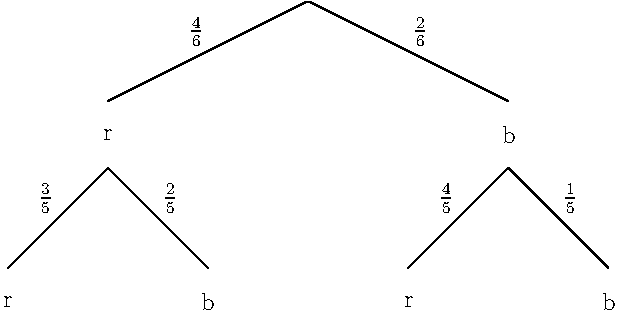
\includegraphics[width=10cm]{dist_marbles_SOL_1.pdf} 
  \end{center}
  \begin{center}
  \begin{tabular}[t]{|c|c|c|c|}
    $x_i$&0&1&2\\\hline
    $F(x_i)$&$\frac26\cdot\frac15=\frac1{15}$&$\frac46\cdot\frac25+\frac26\cdot\frac45=\frac8{15}$&$\frac46\cdot\frac35=\frac6{15}$
  \end{tabular}
\end{center}
\end{Answer}
\answerline{12}
\end{xxwrap}
\vfill

\newpage
\begin{xxwrap}
\begin{exc}
\tr|Elektrische Bauteile werden in 10-er Schachteln verpackt. $4\%$ der Bauteile sind defekt. Sei $X$ die Anzahl defekter Bauteile in einer Box.
    Die Zufallsvariable $X$ hat die Verteilung   $$F(x)=\binom{10}{x}\cdot 0.04^x\cdot 0.96^{10-x} \quad\text{für $x=0,1,\ldots,10$}$$ (siehe nächster Abschnitt). 
    Bestimmen Sie die Wahrscheinlichkeit, dass eine zufällig ausgewählre Box keine defekten Bauteile enthält und die Wahrscheinlichkeit, dass eine zufällig ausgewählte Box
    mindestens ein defektes Bauteil enthält. 
   |Electrical components are produced and packed into boxes of 10. It is known that $4\%$ of the components may be faulty. 
    The random variable $X$ denotes the number of faulty items in the box and has a probability distribution $$F(x)=\binom{10}{x}\cdot 0.04^x\cdot 0.96^{10-x}\quad\text{for $x=0,1,\ldots,10$}$$ 
    Find the probability that a randomly selected box will contain no faulty component and the probability that a randomly selected box will contain at least one faulty component. |
\end{exc}
\begin{Answer}
  \begin{align*}
   F(0)&=\binom{10}{0}\cdot 0.04^0\cdot 0.96^{10}=0.96^{10}\approx 0.66 \\
 1-F(0)&\approx 0.34 
  \end{align*}
\end{Answer}
\answerline{12}
\end{xxwrap}
\vfill

\begin{xxwrap}
\begin{exc}
\tr|Die Anzahl Kunden $X$, die einen bestimmten Laden zwischen 3:00 und 3:03: Uhr betreten habe die Verteilung
   |The number of customers $X$, passing a shop during the period from 3:00 pm to 3:03 pm  shall have the distribution |
\[
P(X=x)=F(x)=\frac{0.2^x\cdot e^{-0.2}}{x!}
\]
\tr|wobei |where | $x\in\mathbb{N}$.
\tr|Beatimmen Sie $F(0)$, $F(1)$ und $F(2)$ und die Wahrscheinlichkeit, dass mindestens 3 Kunden den Laden in der gegebenen Zeitperiode betreten. 
   |Find $F(0)$, $F(1)$ and $F(2)$ and find the probability that at least three customers will pass the shop in the given period. |
\end{exc}
\begin{Answer}
  \begin{align*}
   F(0)&=\frac{0.2^0\cdot e^{-0.2}}{0!}\approx 0.8187\\ 
   F(1)&=\frac{0.2^1\cdot e^{-0.2}}{1!}\approx 0.1637\\ 
   F(2)&=\frac{0.2^2\cdot e^{-0.2}}{2!}\approx 0.0164\\ 
  \end{align*}
  \[
    P(\text{\tr|mindest. 3|at least 3|})= 1-F(0)-F(1)-F(2)\approx 0.0011
  \]
\newpage
\end{Answer}
\answerline{12}
\end{xxwrap}
\vfill

\newpage
% Discrete Probability Distributions:2 ends here

% [[file:../scripts.org::*Binomial and hypergeometric distribution][Binomial and hypergeometric distribution:5]]
\section{\tr|Die Binomialverteilung und die hypergeometrische Verteilung|The binomial and the hypergeometric distribution|}
\begin{xxwrap}
\begin{exc}
 \tr|In einem Behälter befinden sich 6 Kugeln, 4 davon sind rot und 2 schwarz. Sie ziehen 3 Kugeln \textbf{mit Zurücklegen}. Sei $X$ die Anzahl roter Kugeln in ihrer Stichprobe. 
     Zeichen Sie ein Baumdiagamm der Situation und bestimmen Sie die Wahrscheinlichkeitsverteilung der Zufallsvarabeln $X$.  
    |There are 6 balls in a container, 4 of them are red  and 2 are black. You draw a sample of 3 balls \textbf{with replacement}. 
     Let $X$ be the number of red balls in your sample. Draw a tree diagram and find the probability distribution of the random variable $X$. | 
\end{exc}
\begin{Answer}$\,$\\
  \begin{center}
  \tr|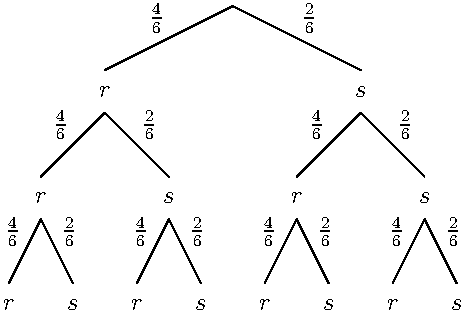
\includegraphics[width=0.5\textwidth]{binomial_01_de.pdf}
  |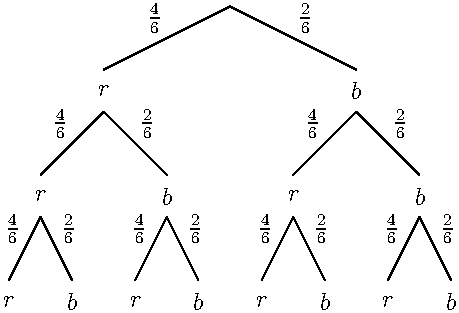
\includegraphics[width=0.5\textwidth]{binomial_01_en.pdf} |
\end{center}
\par\bigskip
\begin{center}
  \begin{tabular}[t]{|r|c|c|c|c|}
   $k$ &0&1&2&3\\\hline
    $F(k)$&$\left(\frac26\right)^3$&$3\left(\frac46\right)\left(\frac26\right)^2$&$3\left(\frac46\right)^2\left(\frac26\right)$&$\left(\frac46\right)^3$
  \end{tabular}
\end{center}
\end{Answer}
\answerline{10}
\end{xxwrap}
\par
\vfill
\begin{xxwrap}
\begin{exc}
\tr|Gleiche Frage, aber diesesmal \textbf{ohne Zurücklegen}.|Same question but \textbf{without replacement}. |
\end{exc}
\begin{Answer}$\,$\\
  \begin{center}
  \tr|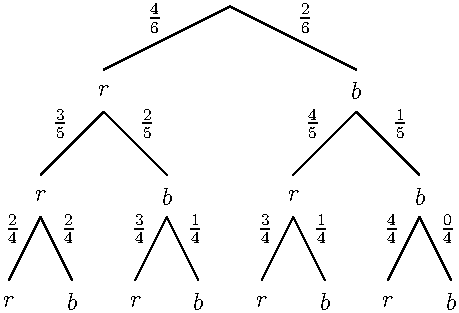
\includegraphics[width=0.5\textwidth]{hyper_01_en.pdf}
  |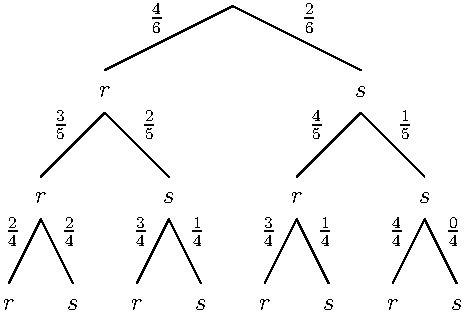
\includegraphics[width=0.5\textwidth]{hyper_01_de.pdf} |
\end{center}
\par\bigskip
\begin{center}
  \begin{tabular}[t]{|r|c|c|c|c|}
   $k$ &0&1&2&3\\\hline
    $F(k)$&$\frac26\frac15\frac04$&$\frac46\frac25\frac14+\frac26\frac45\frac14+\frac26\frac15\frac44$&$\frac46\frac35\frac24+\frac46\frac25\frac34+\frac26\frac45\frac34$&$\frac46\frac35\frac24$
  \end{tabular}
\end{center}
\end{Answer}
\answerline{20}
\end{xxwrap}
\par
\begin{xxwrap}
\begin{exc}
 \tr|Verallgemeinern Sie das Resultat der ersten dieser  Aufgabe (mit Zurücklegen) auf |Generalize the first of these results (with replacement) to |
\renewcommand{\arraystretch}{1}
 \begin{center}
   \begin{tabular}[t]{ll}
     $N$& \tr|Anzahl Kugeln im Behälter|Number of balls in container| \\
     $R$& \tr|Anzahl rote Kugeln in Behälter|Number of red balls in container|\\
     $n$& \tr|Anzahl Kugeln in der Stichprobe|Number of balls in sample|\\
     $r$& \tr|Anzahl rote Kugeln in der Stichprobe|Number of red balls in sample| 
   \end{tabular}
 \end{center}
\end{exc}
\begin{Answer}
  \[
    F(r)=\binom{n}{r}\left(\frac RN\right)^r\left(\frac{N-R}{N}\right)^{n-r}
    = \binom{n}{r}\left(\frac RN\right)^r\left(1-\frac RN\right)^{n-r}
  \]
\end{Answer}
\answerline{15}
\end{xxwrap}
\par
\begin{xxwrap}
\begin{exc}
 \tr|Warum ist es schwierig, die zweite Aufgabe zu verallgemeinern?| Why is it hard to generalize the second result?|
\par
\tr|Sie können das Problem auch folgendermassen anschauen: | We can reformulate the problem:|
\begin{itemize}
\item 
\tr|Auf wieviele Arten können wir $r$ aus $R$ roten Kugeln und $n-r$ aus $N-R$ schwarzen Kugeln auswählen?
     |In how many ways can we choose $r$ out of $R$  red balls and $n-r$ out of $N-R$ black balls? | 
\item
\tr|Auf wieviele Arten können wir $n$ aus $N$ Kugeln auswählen?|In how many ways can we choose $n$ out of $N$ balls?|
\item 
\tr|Und was sagt das aus über die Wahrscheinlichkeit, genau $r$ rote Kugeln zu ziehen?
   |And what does this imply for the probability to draw exactly $r$  red balls?| 
\end{itemize}
\end{exc}
\begin{Answer}
 \tr|Die Wahrscheinlichkeiten hängen vom eingeschlagenen Pfad ab.|The probabilities depend on the paths.|
 \begin{itemize}
 \item
   \[
     \binom Rr \quad\text{\tr|und|and|}\quad \binom{N-R}{n-r}
   \]
 \item
   \[
     \binom Nn
   \]
 \item
   \[
     F(r)=P(X=r)=\frac{\binom Rr\cdot\binom {N-R}{n-r}}{\binom Nn}
   \]
 \end{itemize}
\end{Answer}
\answerline{15}
\end{xxwrap}
\par\bigskip\bigskip\bigskip\bigskip\bigskip
\tr|Wir können das Beispiel mit dem Zurücklegen der Kugeln sogar noch weiter verallgemeinern:
   |We can generalize the example 'with  replacement' even more:|
\begin{itemize}
\item \tr|Jedes Ziehen einer Kugel ist ein eigenständiges Experiment.  |Each draw can be seen as a single experiment.|
\item \tr|Weil wir die Kugel zurücklegen, führen wir jedesmal das gleiche Experiment durch. Die Experimente sind also voneinander unabhängig. 
         |Because we are replacing  the ball,  we perform exactly the same experiment, again and again. These experiments are hence independent. |
\item \tr|Das Experiment hat nur zwei mögliche Ausgänge, \emph{rot} oder \emph{schwarz}, die wir auch etwas allgemeiner \emph{Erfolg} oder \emph{Misserfolg} nennen könnten. 
         |This experiment has only two possible outcomes, \emph{red} or \emph{black}, which we could also call \emph{succcess} or \emph{failure}. |
\end{itemize}
\begin{ttile}{\tr|Binomialverteilung|Binomial Distribution|}
\tr|Ein Experiment habe die Erfolgswahrscheinlichkeit $p$. Sei $X$ die Anzahl Erfolge bei $n$ (unabhängigen) Wiederholungen des Experiments. 
    Die Wahrscheinlichkeit, dass wir bei $n$  Wiederholungen genau $r$ Erfolge haben ist:
   |A certain experiment shall succeed with probability $p$. Let $X$ be the number of successes in $n$ (independent) repetitions of the experiment.
    The probability to have exactly $r$ successes within $n$  repetitions of this experiment is:|
\[
P(X=r)= \binom{n}{r}p^r(1-p)^{n-r}
\]
\tr|Diese Verteilung heisst \textbf{Binomialverteilung}. |This distribution is called \textbf{binomial distribution}|
\end{ttile}
\par\bigskip
\tr|Legt man die Kugeln nicht zurück, so sind die Experimente nicht mehr unabhängig und die Erfolgeswahrscheinlichkeit ist nicht mehr konstant. 
Aber da dieses Modell auf viele reale Situationen passt hat die Verteilung der Anzahl gezogener roter Kugeln einen Namen: 
|If we don't replace the balls, the experiments are not independent anymore and the probability for success is not constant.  
But since this model fits many real life situations, the distribution of the number of drawn red balls has a name:| 

\par\bigskip
\begin{ttile}{\tr|Hypergeometrische Verteilung|Hypergeometric Distribution|}
 \tr|Die Wahrscheinlichkeitsverteilung |The probability distribution | 
\[
P(X=r)=\frac{\binom Rr \binom {N-R}{n-r}}{\binom Nn}
\]
\tr|heisst \textbf{hypergeometrische Verteilung}. |is called \textbf{hypergeometric distribution}.|  
\end{ttile}
\par\vfil
\newpage
\begin{xxwrap}
\begin{exc}
 \tr|Am Zoll:|At the customs:|
 \begin{enumerate}
 \item \tr|Nehmen wir an, Zöllner wissen aus Erfahrung, dass im Schnitt 3 von 10 Fahrern schmuggeln. Wie gross ist die Wahrscheinlichkeit, dass von 5 kontrollierten 
   Fahrern genau 2 schmuggeln.
   |Let's assume that custom officers know by experience that on average 3 out of 10 drivers smuggle. What is the probability that exactly 2 out of 5 selected drivers smuggle? | 
\item \tr|Aufgrund eines Tipps wissen die Zöllner, dass von den nächsten 10 Fahrern tatsächlich genau 4 schmuggeln. Sie kontrollieren 5 der 10 Fahrer. 
Wie gross ist die Wahrscheinlichkeit, dass genau 2 dieser 5 schmuggeln?
|The custom officers got a tip: Within the next 10 drivers, exactly 4 are smugglers. They check 5 of these 10.  What is the probability that exactly 2 of these 5 are smugglers?|
 \end{enumerate}
\end{exc}
\begin{Answer}
  \begin{itemize}
  \item
    \[
      \binom 52\left(\frac3{10}\right)^2\left(1-\frac3{10}\right)^3
    \]
  \item
    \[
      \frac{\binom 42 \binom {6}{3}}{\binom{10}5}
    \]
  \end{itemize}
\newpage
\end{Answer}
\answerline{20}
\end{xxwrap}
% Binomial and hypergeometric distribution:5 ends here

% [[file:../scripts.org::*Expectation][Expectation:1]]
\newpage
\section{\tr|Erwartungwert|Expectation|}
\tr|Wir spielen das folgende Spiel: Sie werfen 2 Würfel und Sie erhalten die Augenzahl in Franken ausbezahlt. Würfeln Sie also eine 4 und eine 3, so bekommen Sie 7 Franken. 
Wenn wir dieses Spiel nun sehr oft spielen, wieviel gewinnen Sie durchschnittlich pro Spiel? Oder anders gefragt, welchen Gewinn pro Spiel können Sie erwarten?
|We play the following game: We roll two dice. You will receive the total number of pips paid out in Swiss francs. So roll a 4 and a 3 to get 7 francs. 
If we play this game very often, what is the average value we get paid per game? Or: What is the value we can expect to receive on average?|
\vsp\vsp


\begin{ttile}{\tr|Erwartungswert|Expected value|}
  \tr|Sei $X$ eine diskrete Zufallsvariable mit den Werten $x_1,x_2,\ldots, x_n$ 
   und $F$ ihre Verteilungsfunktion (d.h. $F(x_i)=P(X=x_i)$). Der \textbf{Erwartungswert} von $X$ is dann definiert durch
|Let $X$ be a discrete random variable with values $x_1,x_2,\ldots, x_n$ 
and $F$ be the probability distribution. (i.e.  $F(x_i)=P(X=x_i)$). The \textbf{expected value} of $X$  is given by|
\end{ttile}

\tr|Oft hat $X$ Werte in $\N$ und dann kann man die Definition einfacher schreiben: 
|Quite often $X$ has its values in $\N$ and then we can write: |
\begin{ttile}{\tr|Erwartungswert vereinfacht|Expected value simpliefied|}
  \tr|Sei $X$ eine diskrete Zufallsvariable mit den Werten $1,2,\ldots, n$ 
   und $F$ ihre Verteilungsfunktion (d.h. $F(i)=P(X=i)$). Der \textbf{Erwartungswert} von $X$ is dann definiert durch
|Let $X$ be a discrete random variable with values $1,2,\ldots, n$ 
and $F$ be the probability distribution. (i.e.  $F(i)=P(X=i)$). The \textbf{expected value} of $X$  is given by|
\[
E(X) = \sum_{i=1}^n i\cdot F(i)=\sum_{i=1}^n i\cdot P(X=i).
\]
\end{ttile}

\vsp\vsp
\tr|Mit $$X=\text{Augensumme}$$ w"are in unserem Beispiel  der Erwartungswert also| With $$X=\text{total number of pips}$$ in our example, the expected value is |
\[
E(X)=2\cdot \frac{1}{36}+3\cdot \frac{2}{36} + 4\cdot \frac{3}{36} + \ldots + 12\cdot \frac{1}{36} = \frac{252}{36}=7.
\]



\begin{example}
\tr|Sie drehen am abgebildeten Glücksrad. Wenn es stoppt erhalten Sie den Betrag, der ausserhalb des Sektors steht, an dem 
das Glücksrad hält. Welchen Gewinn können Sie erwarten? 
|We spin the following wheel of fortune. 
The pointer will stop somewhere and we will receive the amount indicated outside the sector. 
What value do we expect on average, i. e. how much must be paid out on average per game?|
\begin{center}
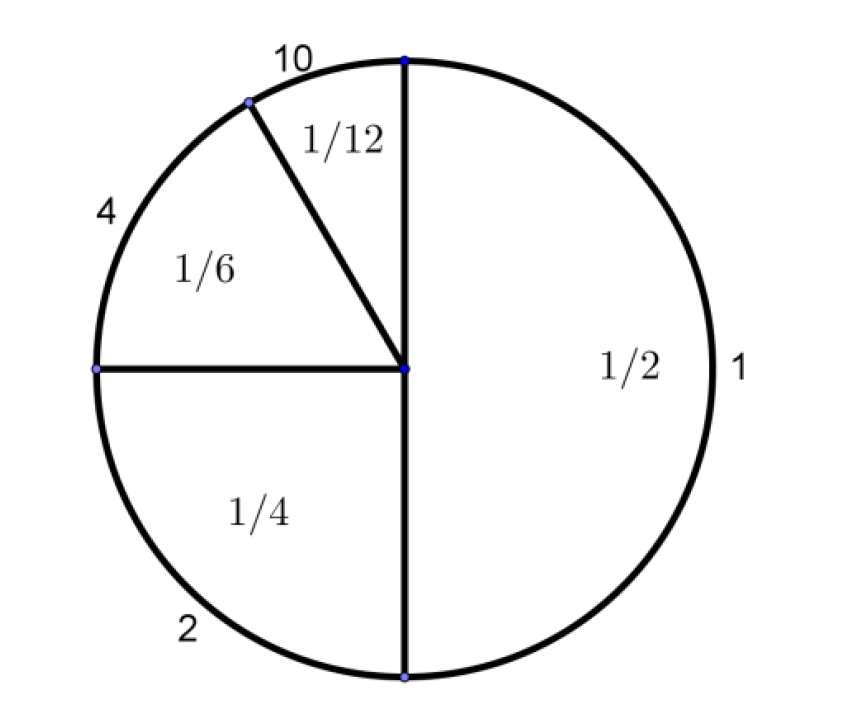
\includegraphics[width=5cm]{Gluecksrad}
\end{center}
\tr|Wenn wir das Glücksrad $m$ mal drehen erhalten wir im Schnitt
|Assume we spin $m$ times. On average, we win|

\begin{itemize}
\item CHF 1.-  in $m\cdot\frac{1}{2}$  \tr|aller Fälle|of all cases|.
\item CHF 2.- in $m\cdot\frac{1}{4}$   \tr|aller Fälle|of all cases|.
\item CHF 4.- in $m\cdot\frac{1}{6}$   \tr|aller Fälle|of all cases|.
\item CHF 10.- in $m\cdot\frac{1}{12}$ \tr|aller Fälle|of all cases|.
\end{itemize}

\tr|Deshalb gewinnt man im Schnitt| Therefore, on average we win|

\[
\frac{m\cdot\frac{1}{2}\cdot 1+m\cdot\frac{1}{4}\cdot 2+m\cdot\frac{1}{6}\cdot 4+m\cdot\frac{1}{12}\cdot 10}{m}=\frac{1}{2}\cdot 1+\frac{1}{4}\cdot 2+\frac{1}{6}\cdot 4+\frac{1}{12}\cdot 10=\text{ CHF }2.50 
\]

\tr|was genau obiger Definition des Erwartungswertes entspricht.| which coincides exactly with the above-mentioned formula.|
\end{example}
\vsp
\begin{xxwrap}
\begin{exc}
\tr|Für das folgende Spiel müssen Sie einen Einsatz von CHF 1.60 zahlen: Eine Münze wir dreimal geworfen. 
Jedesmal, wenn Kopf erscheint erhalten Sie CHF 1. Würden Sie das Spiel annehmen?
|You play the following game, which costs CHF 1.60: 
We throw three times a coin. Each time head occurs, you get CHF 1.- paid out. 
Would you play that game? What is the expected value of that game?|
\end{exc}
\begin{Answer}
  $X=\text{\tr|Anzahl Köpfe|Number of heads|}$
  \begin{center}
    \begin{tabular}[t]{|r|c|c|c|c|}
\hline
      $k$&0&1&2&3\\\hline
      $P(X=k)$&$\frac18$&$\frac38$&$\frac38$&$\frac18$\\\hline
    \end{tabular}
  \end{center}
\[
E(X)=0\cdot\frac18+1\cdot\frac38+2\cdot\frac38+3\cdot\frac18=\frac{12}8=1.5
\]
\tr|Der Erwartungswert ist kleiner als die Kosten des Spieles, ich würde es also nicht spielen.|The expected value is smaller than the cost, I wouldn't play the game.|
\end{Answer}
\answerline{12}
\end{xxwrap}
\vfill

\begin{xxwrap}
\begin{exc}
  \tr|Jedesmal, wenn Sie das folgende Glücksrad drehen, müssen Sie einen Franken zahlen und Sie bekommen den Betrag, 
der in dem Sektor steht in dem der Zeiger des Glücksrades am Schluss steht. Was ist der Erwartungswert dieses Spiels?
  |We spin the following wheel of fortune.
   Each time we spin, we have to pay CHF 1.- 
   and we get paid out the amount of money written within the sector the pointer stops.
   What is the expected value of that game?|
\begin{center}
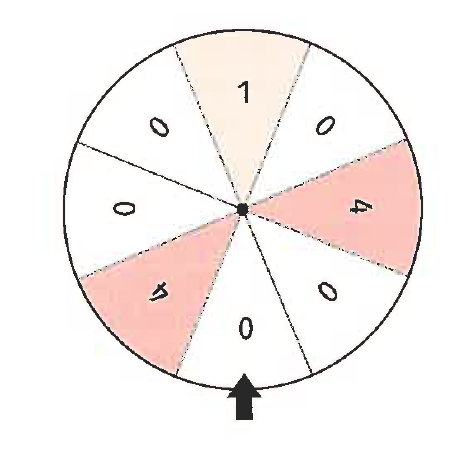
\includegraphics[width=5cm]{Wheel1}
\end{center}
\end{exc}
\begin{Answer}
  \[
    E(X)=(1+4+4)\frac18-1=0.125
  \]
\end{Answer}
\answerline{12}
\end{xxwrap}



\begin{exc}
\tr|Ein Gl"ucksrad hat 4 gleichgrosse Sektoren in den die jeweiligen Gewinne  0,2,4 und 8 stehen.
   |A wheel of fortune has four sectors with values 0, 2, 4 and 8 written in it. Again, the number indicates the amount of money paid out. |
\begin{enumerate}
\item 
\tr|Welchen Betrag sollte es kosten, das Gl"ucksrad zu drehen, damit das Spiel \emph{fair} ist, d. h. Erwartungswert 0 hat?
   |What should spinning the wheel cost such that the game is \emph{fair} (i.e. that the expected value is zero)?|
\item 
\tr|Nehmen wir an, es koste CHF 2.50 das Gl"ucksrad zu drehen. Finden Sie eine m"ogliche Aufteilung der Sektoren, so dass das Spiel fair ist. 
   |Let's say, one has to pay CHF 2.50 to spin the wheel. Determine one possible subdivision of the sectors such that the game is fair. |
\end{enumerate}
\begin{center}
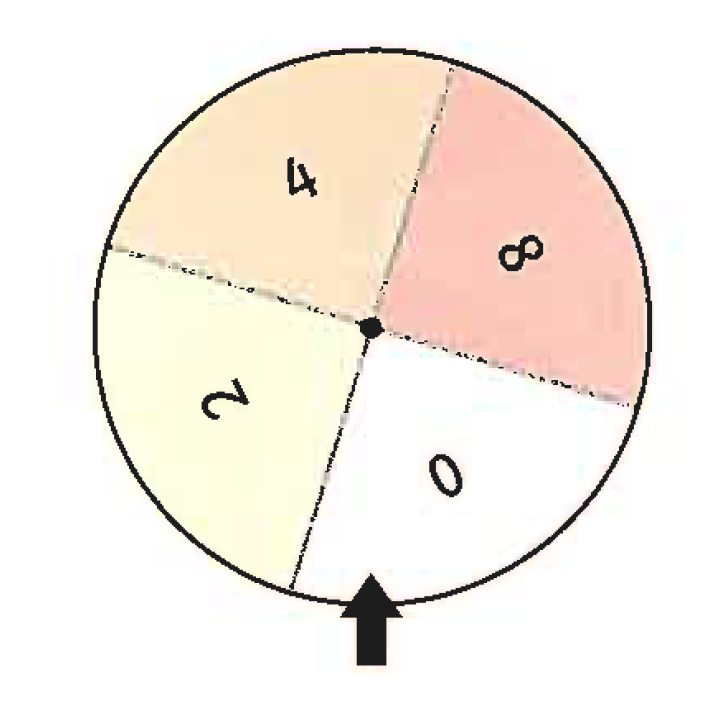
\includegraphics[width=5cm]{Wheel2}
\end{center}
\end{exc}
\begin{Answer}
  \begin{enumerate}
  \item
    \[
      E(X)=(0+2+4+8)\frac14=\frac{14}4=3.5
    \]
    \tr|Das Spiel sollte CHF 3.50 kosten.|The game should cost CHF 3.50.|
  \item
    \tr|Z.\,B. vier gleichgrosse Sektoren mit der Belegung 0, 0, 0, 10.|
        E.\,g. four sectors of equal size with numbers 0, 0, 0, 10.|
  \end{enumerate}
\end{Answer}
\answerline{12}



\begin{xxwrap}
\begin{exc}\label{petersburg}
\tr|Berechnen Sie den erwarteten Gewinn im St. Petersburg Paradox (Übung \ref{petersburgintro}).
   |Find the expected win in the St. Petersburg paradox (exercise \ref{petersburgintro}).|
\end{exc}
\begin{Answer}
  \begin{align*}
    E(X)=&2\cdot P(T)\\
         &+4\cdot P(HT)\\
         &+8\cdot P(HHT)\\
         &+\dots\\
    =&2\cdot\frac12 \\
         &+4\cdot\frac14\\
         &+8\cdot\frac18\\
         &+\ldots\\
    =&1+1+1+\ldots=\infty
  \end{align*}
\end{Answer}
\answerline{12}
\end{xxwrap}
% Expectation:1 ends here

% [[file:../scripts.org::*Linearity of expectation][Linearity of expectation:1]]
\subsection{\tr|Linearität des Erwartungswertes|Linearity of expectation|}
\begin{xxwrap}
\begin{exc}\label{altexp}
\tr|Beweisen Sie die folgende alternative Charakterisierung:  |Prove the following alternative characterisation:| 
\[
E(X)=\sum_{\omega\in\Omega}X(w)P({w})
\]
\end{exc}
\begin{Answer}
  \begin{align*}
    E(X)&=\sum_{\omega\in\Omega}X(\omega)P({\omega})\\
    &=\sum_k\sum_{\omega\in\Omega:X(\omega)=k}X(\omega)P({\omega})\\
    &=\sum_k\sum_{\omega\in\Omega:X(\omega)=k}kP({\omega})\\
    &=\sum_kk\sum_{\omega\in\Omega:X(\omega)=k}P({\omega})\\
    &=\sum_kkP(X=k)
  \end{align*}
\end{Answer}
\answerline{6}
\end{xxwrap}

\begin{xxwrap}
\begin{exc}
\tr|Beweisen Sie, dass der Erwartungswert linear ist:  |Prove that expectation is linear:| 
\begin{align*}
E(X_1+X_2)&=E(X_1)+E(X_2)\\
E(cX)&=cE(X)
\end{align*}
\tr|Hinweis: Verwenden Sie Übung|Hint: Use | \ref{altexp} 
\end{exc}
\begin{Answer}
  \begin{align*}
    E(X_1+X_2)&=\sum_{\omega\in\Omega}\left(X_1+X_2\right)\omega)P({\omega})\\
    &=\sum_{\omega\in\Omega}\left(X_1(\omega)+X_2(\omega)\right)P({\omega})\\
    &=\sum_{\omega\in\Omega}X_1(\omega)P({\omega})
               +\sum_{\omega\in\Omega}X_2(\omega)P({\omega})\\
              &=E(X_1)+E(X_2)\\
    E(cX)&=\sum_{\omega\in\Omega}(cX)(\omega)P({\omega})\\
    &=\sum_{\omega\in\Omega}cX(\omega)P({\omega})\\
    &=c\sum_{\omega\in\Omega}X(\omega)P({\omega})\\
              &=cE(X)
  \end{align*}
\end{Answer}
\answerline{6}
\end{xxwrap}

\vsp\vsp
\begin{xxwrap}
  \begin{exc}
    \tr|Das obige Spiel kann man auch als Summe zweier einfacherer Spiele mit nur einem Würfel sehen.
    Seien $X_1$ und $X_2$ die jeweiligen Augensummen der einzelnen Würfel.
    |You can see the previous game as the sum of two simpler games: Let $X_1$ and $X_2$ be the number of pips on the respective dice.| 
    \begin{itemize}
    \item \tr|Berechnen Sie $E(X_1)$ und $E(X_2)$|Compute $E(X_1)$ and $E(X_2)$|.
    \item \tr|Berechnen Sie | Compute |$E(X)$. 
    \end{itemize}
  \end{exc}
  \begin{Answer}
    \begin{itemize}
    \item
      \[
        E(X_1)=E(X_2)=1\cdot\frac16+2\cdot\frac16+3\cdot\frac16+4\cdot\frac16+5\cdot\frac16+6\cdot\frac16=(1+2+3+4+5+6)\frac16=21\cdot\frac16=\frac72
      \]
    \item
      \[
        E(X_1)+E(X_2)=\frac72+\frac72=7
      \]
    \end{itemize}
  \end{Answer}
  \answerline{12}
\end{xxwrap}
% Linearity of expectation:1 ends here

% [[file:../scripts.org::*Expectation of a binomially distributed random variable][Expectation of a binomially distributed random variable:1]]
\subsection{\tr|Erwartungswert einer binomial verteilten Zufallsvariabeln|Expectation of a binomially distributed random variable|}
\begin{xxwrap}
\begin{exc}
\tr|In einer bestimmten Gegend der Welt sei die Wahrscheinlichkeit, dass es an einem Tag regnet 0.28. 
Wieviele Regentage erwarten Sie pro Jahr?
|In a particular region, the probability that it will rain on any one day is 0.28. 
On how many days of the year would you expect it to rain?|
\end{exc}
  \begin{Answer}
   \(0.28\cdot 365=102.2\) 
  \end{Answer}
\answerline{12}
\end{xxwrap}
\vfill


\begin{xxwrap}
\begin{exc}
\tr|Wenn zwei Würfel gleichzeitig 180  mal gewürfelt werden, wie oft erwarten Sie identische Augenzahlen?
|If two dice are rolled simultaneously 180 times, 
on how many occasions would you expect to get twice the same number of pips?|
\end{exc}
\begin{Answer}
  \tr|Intuitiv: In $\frac6{36}=\frac16$ aller Fälle werfen wir identische Augenzahlen, insgesamt in $\frac16\cdot180=30$ Fällen.
     |Intuitively: In $\frac6{36}=\frac16$ of the cases we throw the same number of pins , i.e. in $\frac16\cdot180=30$ cases.|
\par
\tr|Formal: Sei $X$ die Anzahl Würfe mit identischen Augenzahlen nach 180 Würfen. Dann ist 
   |Formally: Let $X$ be the number of throws with the same mumber of pins. Then | 
\[
X=X_1+X_2+\ldots+X_{180}
\]
\tr|wobei die Zufallsvariabeln $X_i$ definiert sind durch|where the random variables $X_i$ are defined as|
\[
X_i=\left\{
\begin{array}{ll}
 1 & \text{\tr|gleiche Augenzahl in Wurf $i$|same number of pins in throw number $i$|}\\
 0 & \text{\tr|sonst|else|}
\end{array}\right.
\] 
\tr|Die $X_i$ haben alle den gleichen Erwartungswert:|The $X_i$ all have the same expected value:|
\[
E(X_i)=0\cdot P(X=0)+1\cdot P(X=1)=P(X=1)=\frac6{36}
\]
\tr|und das Resultat folgt aus der Linearität des Erwartungswertes. | and the result follows from the linearity of the expected value. |
\end{Answer}
\answerline{12}
\end{xxwrap}
\vfill
\begin{ttile}{\tr|Erwartungswert einer binomial verteilten Zufallsvariabeln |Expectation of a binomially distributed random variable|}
\tr|Sei $X$ eine binomial verteilte Zufallsvariable |Let $X$ be a binomially distributed random variable|
   \[
     P(X=k)=\sum_{k=0}^n\binom{n,k}kP(X=k)
   \]
\tr|dann gilt für ihren Erwartungswert |then|
\[
E(X)=np
\]
\end{ttile}

\begin{xxwrap}
  \begin{exc}
    \tr|Beweisen Sie obige Formel.| Prove this formula.|
    \begin{enumerate}
    \item \tr|Versuchen Sie zuerst direkt die Definition des Erwartungswertes anzuwenden.
              Dabei entsteht eine einschüchternde Formel.
             |First try to use the definition of expectation directly.
              The resulting formula is rather intimidating. |
    \item \tr|Zerlegen Sie $X$ in einfachere Zufallsvariabeln:|Decompose $X$ in simpler random variables:|
      \[
        X=X_1+x_2+\cdots+X_n
      \]
      \tr|mit|with|
      \[
        X_i=
        \begin{cases}
          1 & \text{\tr|Experiment \#$i$ ist ein Erfolg|experiment \#$i$ is a success|}\\
          0 & \text{\tr|sonst|else|}
        \end{cases}
      \]
      \tr|Verwenden Sie dann die Linearität des Erwartungswertes.|Then use linearity of expectation.|
    \end{enumerate}
  \end{exc}
  \begin{Answer}
   \[
   E(X_i)=0\cdot P(X=0) + 1 \cdot P(X=1) = p 
   \]
   \[
   E(X)=np
   \] 
  \end{Answer}
  \answerline{12}
\end{xxwrap}
% Expectation of a binomially distributed random variable:1 ends here

% [[file:../scripts.org::*Expectation of a hypergeometrically distributed random variable][Expectation of a hypergeometrically distributed random variable:1]]
\subsection{\tr|Erwartungswert einer hypergeometrisch verteilten Zufallsvariablen|Expectation of a hypergeometrically distributed random variable|}
\begin{ttile}{\tr|Erwartungswert einer hypergeometrisch verteilten Zufallsvariabeln |Expectation of a hypergeometrically distributed random variable|}
\tr|Sei $X$ eine hypergeometrisch  verteilte Zufallsvariable |Let $X$ be a hypergeometrically distributed random variable|
   \[
     P(X=r)=\frac{\binom Rr \binom {N-R}{n-r}}{\binom Nn}
   \]
\tr|dann gilt für ihren Erwartungswert |then|
\[
E(X)=n\frac RN
\]
\end{ttile}

\begin{xxwrap}
  \begin{exc}
    \tr|Beweisen Sie obige Formel.| Prove this formula.|
    \begin{enumerate}
    \item \tr|Versuchen Sie zuerst direkt die Definition des Erwartungswertes anzuwenden.
              Dabei entsteht wieder eine einschüchternde Formel.
             |First try to use the definition of expectation directly.
              The resulting formula is again rather intimidating. |
    \item \tr|Zerlegen Sie $X$ wieder in einfachere Zufallsvariabeln:
              Das Problem ist nur wie? Die Zufallsvariabeln $X_i$ aus der entsprechenden Aufgabe für die Binomialverteilung haben Verteilungen die voneinander abhängen.
              Der überraschende Ausweg besteht darin den Standpunkt zu wechseln: Statt das Experiment aus der Sicht der 'Ziehenden' zu betrachten, schauen wir es aus der Sicht einer roten Kugel an: 
             |Decompose $X$ again in simpler random variables: The only problem is: how could we do that? The random variables $X_i$ from the corresponding exercise on binomially distributed 
              random variables have distributions that depend on each other. The surprising solution is to shift the point of view: instead of looking at the experiment from outside we look at it 
              from the point of view of a red ball:|
          \[
            X=X_1+X_2+\cdots+X_R
          \]
          \tr|mit|with|
          \[
            X_i=
            \begin{cases}
              1 & \text{\tr|Die rote Kugel \#$i$ wird gezogen|red ball \#$i$ is drawn|}\\
              0 & \text{\tr|sonst|else|}
            \end{cases}
          \]
          \tr|Verwenden Sie dann die Linearität des Erwartungswertes.|Then use linearity of expectation.|
    \end{enumerate}
  \end{exc}
  \begin{Answer}
   \[
   E(X_i)=\frac nN
   \]
   \[
   E(X)=R\frac nN=n\frac RN
   \] 
  \end{Answer}
  \answerline{12}
\end{xxwrap}

\begin{xxwrap}
  \begin{exc}
    \tr|Die Formeln für die Erwartungswerte von binomial und hypergeometrisch verteilten Zufallsvariabeln
    sind konsistent in welchem Sinne?
    |The formulas for the expectations of binomially and hypergeometrically distributed random variable are in a certain sense consistent, can you see how?|
  \end{exc}
  \answerline 8
  \begin{Answer}
    \tr|Wenn wir die Binomialverteilung im 'Kugelmodell' interpretieren, dann ist die Erfolgswahrscheinlichkeit gerade
       |If we interpret the binomial distribution in the 'ball-model', then the success probability is exactly|
       \[
         p=\frac RN
       \]
  \end{Answer}
\end{xxwrap}
% Expectation of a hypergeometrically distributed random variable:1 ends here

% [[file:../scripts.org::*Epilogue][Epilogue:1]]
\ifANSWERS
\ifAnswersAtEnd
\newpage\section{\tr|L"osungen|Solutions|}
\shipoutAnswer
\fi\fi
\end{document}
% Epilogue:1 ends here
